%%%%%%%%%%%%%%%%%%%%%%% file template.tex %%%%%%%%%%%%%%%%%%%%%%%%%
%
% This is a general template file for the LaTeX package SVJour3
% for Springer journals.          Springer Heidelberg 2010/09/16
%
% Copy it to a new file with a new name and use it as the basis
% for your article. Delete % signs as needed.
%
% This template includes a few options for different layouts and
% content for various journals. Please consult a previous issue of
% your journal as needed.
%
%%%%%%%%%%%%%%%%%%%%%%%%%%%%%%%%%%%%%%%%%%%%%%%%%%%%%%%%%%%%%%%%%%%
%
% First comes an example EPS file -- just ignore it and
% proceed on the \documentclass line
% your LaTeX will extract the file if required
\begin{filecontents*}{example.eps}
%!PS-Adobe-3.0 EPSF-3.0
%%BoundingBox: 19 19 221 221
%%CreationDate: Mon Sep 29 1997
%%Creator: programmed by hand (JK)
%%EndComments
gsave
newpath
  20 20 moveto
  20 220 lineto
  220 220 lineto
  220 20 lineto
closepath
2 setlinewidth
gsave
  .4 setgray fill
grestore
stroke
grestore
\end{filecontents*}
%
\RequirePackage{fix-cm}
%
%\documentclass{svjour3}                     % onecolumn (standard format)
%\documentclass[smallcondensed]{svjour3}     % onecolumn (ditto)
%\documentclass[smallextended]{svjour3}       % onecolumn (second format)
\documentclass[twocolumn]{svjour3}          % twocolumn
%
\smartqed  % flush right qed marks, e.g. at end of proof
%
%\usepackage{graphicx}
\usepackage{hyperref}
\usepackage{float}
\usepackage{verbatim} %comments

\usepackage{graphicx}
%\usepackage[pdftex]{graphicx}
% declare the path(s) where your graphic files are
%\graphicspath{{./Figures/Pdf/}{}}
  % and their extensions so you won't have to specify these with
  % every instance of \includegraphics
%\DeclareGraphicsExtensions{.pdf,.jpeg,.png}


% *** MATH PACKAGES ***
%
%\usepackage{amsthm}
\usepackage{amsmath}
\usepackage{amssymb}

%\newtheorem{definition}{Definition}
\newtheorem{thm}{Theorem}[section]
\newtheorem{lem}[thm]{Lemma}

%tutorial: https://tex.stackexchange.com/questions/43966/how-to-make-the-optional-title-of-a-theorem-bold-with-amsthm


% *** SPECIALIZED LIST PACKAGES ***
\usepackage{algorithmicx}
\usepackage{algorithm}
\usepackage[noend]{algpseudocode} % http://ctan.org/pkg/algorithmicx

% *** ALIGNMENT PACKAGES ***
%
\usepackage{array}


% *** FLOAT PACKAGES ***
%
%\usepackage{fixltx2e}
\usepackage{float}

% *** PDF, URL AND HYPERLINK PACKAGES ***
%
\usepackage{url}
% url.sty was written by Donald Arseneau. It provides better support for
% handling and breaking URLs. url.sty is already installed on most LaTeX
% systems. The latest version and documentation can be obtained at:
% http://www.ctan.org/pkg/url
% Basically, \url{my_url_here}.
\usepackage{caption}
\usepackage{mathtools}
\DeclarePairedDelimiter\ceil{\lceil}{\rceil}
\DeclarePairedDelimiter\floor{\lfloor}{\rfloor}

\usepackage{adjustbox}
\usepackage{subcaption}
\captionsetup[subfigure]{labelformat = parens, labelsep = space, font = small}
\usepackage{dirtytalk}
\usepackage[utf8]{inputenc}
\usepackage{pgfplotstable}
%\usepackage{tikz}

% multi row package
\usepackage{multirow}

%color package
\usepackage{xcolor}


%
% \usepackage{mathptmx}      % use Times fonts if available on your TeX system
%
% insert here the call for the packages your document requires
%\usepackage{latexsym}
% etc.
%
% please place your own definitions here and don't use \def but
% \newcommand{}{}
%
% Insert the name of "your journal" with
% \journalname{myjournal}
%
\pgfplotsset{compat=1.18}
\begin{document}

\title{A New Tree-Based Approach to Mine Sequential Patterns%\thanks{Grants or other notes
%about the article that should go on the front page should be
%placed here. General acknowledgments should be placed at the end of the article.}
}
%\subtitle{Do you have a subtitle?\\ If so, write it here}

\titlerunning{A New Tree-Based Approach to Mine Sequential Patterns}        % if too long for running head

\author{Redwan Ahmed Rizvee \and
        Chowdhury Farhan Ahmed \and
        Md. Fahim Arefin \and
        Carson K. Leung
}

%\authorrunning{Short form of author list} % if too long for running head

\institute{Redwan Ahmed Rizvee,  Chowdhury Farhan Ahmed, Md. Fahim Arefin   \at
              Department of Computer Science and Engineering \\
              University of Dhaka, Bangladesh\\
              \email{rizveeredwan.csedu@gmail.com, farhan@du.ac.bd, f.arefin8@gmail.com}           %  \\
%             \emph{Present address:} of F. Author  %  if needed
            \and
            Carson K. Leung \at
              Department of Computer Science\\
              University of Manitoba, Canada \\
              \email{kleung@cs.umanitoba.ca}           %  \\
%             \emph{Present address:} of F. Author  %  if needed
}

%\date{Received: date / Accepted: date}
% The correct dates will be entered by the editor


\maketitle

\begin{abstract}
Sequential Pattern Mining is a popular research domain due to its increasing range of applications. In this article, we have introduced a new tree-based solution to the sequential pattern mining problem, including two sets of novel solutions for static and incremental sequential databases. We have proposed two new structures, \textit{SP-Tree} and \textit{IncSP-Tree} and designed two efficient algorithms, \textit{Tree-Miner} and \textit{IncTree-Miner} to mine the complete set of sequential patterns from static and incremental databases. The proposed novel structures provide an efficient manner to store the complete sequential database maintaining ``build-once-mine-many" property and give scope to perform interactive mining. Additionally a new breath-first based support counting technique has been designed to efficiently identify the infrequent patterns at the early stage and a new heuristic pruning strategy to reduce pattern search space. We have also designed a new pattern storage structure \textit{BPFSP-Tree} to store the frequent patterns during successive iterations in incremental mining to reduce the number of database scans and to remove the infrequent patterns efficiently. A novel structure named Sequence Summarizer is also introduced to efficiently calculate and update the co-occurrence information of the items, especially in an incremental environment. Experimental results over various real-life and synthetic datasets demonstrate the efficiency of our work in comparison with the related state-of-the-art approaches.

\keywords{Sequential Pattern \and Tree-based mining \and Incremental mining \and Breadth-first based pruning \and Pattern Storage}
% \PACS{PACS code1 \and PACS code2 \and more}
% \subclass{MSC code1 \and MSC code2 \and more}
\end{abstract}

\section{Introduction}\label{sec:introduction}
% Computer Society journal (but not conference!) papers do something unusual
% with the very first section heading (almost always called "Introduction").
% They place it ABOVE the main text! IEEEtran.cls does not automatically do
% this for you, but you can achieve this effect with the provided
% \IEEEraisesectionheading{} command. Note the need to keep any \label that
% is to refer to the section immediately after \section in the above as
% \IEEEraisesectionheading puts \section within a raised box.




% The very first letter is a 2 line initial drop letter followed
% by the rest of the first word in caps (small caps for compsoc).
%
% form to use if the first word consists of a single letter:
% \IEEEPARstart{A}{demo} file is ....
%
% form to use if you need the single drop letter followed by
% normal text (unknown if ever used by the IEEE):
% \IEEEPARstart{A}{}demo file is ....
%
% Some journals put the first two words in caps:
% \IEEEPARstart{T}{his demo} file is ....
%
% Here we have the typical use of a "T" for an initial drop letter
% and "HIS" in caps to complete the first word.
The idea of pattern mining problem was introduced to discover interesting characteristics or behavior from the database. Due to the wide variation of database characteristics pattern mining problem has been divided into numerous sub-domains, among which Sequential Pattern Mining (SPM) problem stands out because of its wide range of variations. SPM problem targets to discover frequent sequential patterns from an ordered or sequential database. In Table \ref{table:example_static_database}, we have shown an example of a camera market sequential database where each entry denotes a customer's purchase history. Items within same bracket denotes a transaction for that customer. So, a record is a collection of ordered transactions for that customer. SPM problem will try to discover different types of ordered relationships from this dataset, such as the generic SPM problem will try to discover the ordered item clusters which are frequently purchased. Being first introduced in \cite{srikant1996mining} based on market basket analogy, the SPM problem has found its usage in numerous applications, e.g., web usage mining, customer behavior analysis, DNA sequence mining, etc.

Due to having numerous applications, a wide range of literature has addressed SPM problem and provided solutions which can be broadly categorized into two groups: apriori based and pattern growth based. Apriori based approaches follow candidate generation and testing paradigm and pattern growth approaches follow the projected database or database shrink concept with pattern's gradual extension. Pattern growth approaches are significantly faster compared to apriori approach \cite{borgelt2005implementation}. In traditional itemset mining it has been shown that tree structure alike approaches provide more control over the database which ultimately helps improve the mining runtime\cite{leung2007cantree,borgelt2005implementation} and incorporate new strategies. But due to the problem complexity, the tree alike structures of the itemset mining were not suitable for SPM problem and a structural solution was yet to be proposed. Based on this motivation, in this study, we have proposed a novel tree structure \textit{SP-Tree} to represent the sequential database in a structured format and an efficient mining algorithm \textit{Tree-Miner} to mine sequential patterns using the node properties of \textit{SP-Tree}. The advantage of the proposed tree structure is, it provides efficient structured control over the database and pattern space which ultimately leads to a faster generation of the patterns. An important motivation behind designing such a structure was, if we had a structured format of the database, it would have given the advantage to adopt new pruning strategies and control the manipulation of the database when the database can change based on other parameters, e.g, incremental database, stream database, etc. Our incremental solution is the result of prior motivation.



\begin{table*}[!t]
\parbox{.5\linewidth}{
\centering
\begin{tabular}{|c|c|}
\hline
sid & Sequence\\
\hline
1 & \textless (camera, kit lens) \\
& (50 mm prime lens)   \\
& (tripod) \textgreater\\
\hline
2 & \textless (camera, kit lens)   \\
& (85 mm prime lens) \\
& (tripod) \textgreater \\
\hline
3 & \textless (camera, kit lens)\\
& (tripod) \textgreater \\
\hline
4 & \textless (camera, kit lens) \\
& (50 mm prime lens) \\
& (85 mm prime lens) \textgreater \\
\hline
\end{tabular}
\caption{Initial Camera Market Dataset} \label{table:example_static_database}
}
\hfill
\parbox{.5\linewidth}{
\centering
\begin{tabular}{|c|c|c|}
\hline
sid & New Sequence & Type\\
\hline
1 & \textless (ND Filter, Reverse Ring) \textgreater & Append\\
\hline
2 & $\phi$ & - \\
\hline
3 & $\phi$ & - \\
\hline
4  & $\phi$ & - \\
\hline
5 & \textless (camera, kit lens) \textgreater & Insert\\
\hline
\end{tabular}
\caption{Additional update in Database} \label{table:example_incremental_database}
}
\end{table*}

Generic SPM problem focuses on mining frequent sequential patterns from the static sequential databases
\cite{rizvee2020tree,srikant1996mining,zaki2001spade,han2001prefixspan,fournier2014fast,chen2009updown,perera2008clustering,okolica2018sequence,guidotti2018personalized}. But in real-life applications, most of the time, the database is found not to be static; rather gets increased time to time with more information \cite{mallick2013incremental}. With increased database size, patterns' distribution can vary significantly which necessitates the urge to mine again over the updated complete database. But, mining sequential patterns over the complete database is a very costly operation. So re-mining over the updated database again from scratch creates several performance and resource bottleneck. From these motivations the problem of Incremental Sequential Pattern Mining (ISPM) was introduced in \cite{wang1997discovering} to tackle the challenge of re-mining over the complete database rather than focusing more over the efficient handling of the new incremental database or increased part of the database \cite{mallick2013incremental,slimani2013sequential,fournier2017survey,huang2008general}.

In Table \ref{table:example_incremental_database}, we have shown an example of incremental version of our prior static database shown in Table \ref{table:example_static_database}. Here, two sequences newly appeared. First one as an appended sequence to the existing sequence with identifier ($sid$) 1 and the fifth one is an inserted sequence with a new $sid(5)$ which increases database length. $\phi$ means there was no new sequence as appended or inserted for the corresponding $sid$. Here the updated incremental database will be the concatenation of two databases. The solutions to the ISPM problems focus on developing new strategies to efficiently discover the complete set of updated frequent patterns from this modified database rather than re-mining from scratch.

There are several crucial challenges in ISPM problems due to the problem's nature. For example - handling the modification of existing sequences ($Append$), the addition of completely new appearing sequences ($Insert$), ratio of the incremental database vs existing database, updating the existing data structures, the change in the frequent patterns' distribution or concept drift, empirically setting the extra introduced parameters to control the candidate buffers
\cite{cheng2004incspan,lin2015incrementally} etc. In summary, several issues exist which control the efficiency, applicability and complexity of the solution to approach the ISPM problems and thus numerous literature have addressed this problem \cite{lin2004incremental,cheng2004incspan,liu2012incremental,lin2015incrementally,saleti2019mapreduce}. In this study, we have also proposed a new tree-based solution, \textit{IncTree-Miner} based on \textit{IncSP-Tree} to approach the ISPM problem which provides an efficient manner and structural advantage to implicitly track the incremental database and the patterns which are affected by it.


The usage of co-occurrence information can significantly reduce the search space which has been discussed in many literature\cite{fournier2014fast,fournier2017survey,saleti2019mapreduce}. Our solutions have also adopted this concept. This information states the relationship among the items which guides during pattern extension. But it becomes a challenge on how to efficiently update this information for a gradually increasing database. To solve this issue, we have proposed a novel structure \textit{Sequence Summarizer} which helps calculate such information efficiently especially in an incremental environment. This novel structure is also helpful to perform the \textit{Append} operation over the existing sequences.

The main challenges of any SPM problem are reducing the number of database ($DB$) scans, making the $DB$ scans faster, reducing the search space, and detecting the infrequent patterns early during support calculation. In our proposed structures we have introduced the idea of $next\_link$ which makes the DB scans significantly faster. Also utilizing the tree properties we have developed two new pruning strategies: a breadth-first based support counting technique which helps detect the infrequent patterns early before calculating complete support and a heuristic strategy to reduce the search space.

As, with database increment, the support of the patterns gets updated in each iteration, popular literature maintain a tree alike structure to keep the patterns' support \cite{chen2007incremental,liu2012incremental,lin2015incrementally}. In this study, we further investigate this approach and design a new Bi-directional Projection Pointer Based Frequent Sequential Pattern Tree (\textit{BPFSP-Tree}) which keeps the frequent sequential patterns, their support, and projection pointers using the node structure of \textit{IncSP-Tree}. It helps reduce the number of DB scans and provides an efficient mechanism to remove the non-frequent patterns which were previously frequent.


Because of various crucialities of the ISPM problem, different literature have adopted different types of strategies to solve them. Among them, many introduced additional parameters or concepts such as negative border \cite{zheng2002algorithms}, semi-buffer \cite{cheng2004incspan}, pre-large with upper and lower thresholds \cite{lin2015incrementally} etc. The main problem of additional parameters is that the solution's performance and complexity largely depend on the appropriate selection of these parameters and their mutual dependency and it is difficult to estimate database characteristics prior. Also, these approaches are severely affected due to concept drift and create resource misuse and bottleneck.  Based on these observations, we wanted to reduce the parameters' dependency and stick to the single traditional support threshold parameter. Besides, our approach is a new take to generic SPM problem. So, it is also flexible to other modules. Moreover, our proposed structure stores the complete database in an efficient format. So, it is also able to handle the absence of prior database in stream mining and runtime threshold parameter change. In summary, our main contributions are as follows -

\begin{enumerate}
    \item We have proposed two new tree-based solutions, an efficient \textit{Tree-Miner} algorithm based on a novel tree structure \textit{SP-Tree} and an efficient \textit{IncTree-Miner} algorithm based on a novel tree structure \textit{IncSP-Tree} to solve the SPM problem for static and incremental databases, respectively.
    \item Based on the tree properties, we have designed two new pruning strategies: an efficient breadth-first based support counting technique and and a heuristic pruning strategy.
    \item A novel structure \textit{Sequence Summarizer} is proposed to efficiently calculate and update the co-occurrence information and perform $Append$ operation during database increment.
    \item A new structure \textit{BPFSP-Tree} to store the frequent sequences along with projection pointers to reduce the DB scan and efficiently remove the infrequent patterns.
    \item A Discussion regarding efficiency and effectiveness of our proposed solutions and issues related to implementation.
\end{enumerate}

The preliminary version of the current study has been published in \cite{rizvee2020tree}. These two literature focuses on designing new tree-based solutions to approach the SPM problem by providing a new viewing angle. The prior study proposed a tree-based solution to solve static SPM problem while the current literature has added the following new materials,

\begin{itemize}
    \item More detailed and comprehensive discussion with additional examples to discuss \textit{Tree-Miner} algorithm based on SP-Tree to solve the static SPM problem.
    \item Addition of two new pruning strategies based on SP-Tree structures.
    \item A novel approach to solve the incremental SPM problem with a new incremental mining algorithm \textit{IncTree-Miner} over an extended SP-Tree structure, \textit{IncSP-Tree} with additional discussion about various crucial aspects related to implementation and incremental environment.
    \item More detailed and extensive experimental results to discuss the novelty of the proposals along with more examples, analysis and discussion.
\end{itemize}

% and issues related to the implementations and improvisations.
The rest of the paper is organized as follows. Related works are discussed in Section \ref{related_works}. We formulate our addressed problem in section \ref{problem_definition} and discuss our proposals in Section \ref{proposals}. In Section \ref{evaluation}, we evaluate our solutions based on various metrics by conducting experiments on both real-life and synthetic datasets and finally we conclude this study with an overall summary and the possibility of future extensions in Section \ref{conclusion}.

%\subsection{Subsection Heading Here}
%Subsection text here.

% needed in second column of first page if using \IEEEpubid
%\IEEEpubidadjcol

%\subsubsection{Subsubsection Heading Here}
%Subsubsection text here without citation \cite{rasheed2010efficient}

% An example of a floating figure using the graphicx package.
% Note that \label must occur AFTER (or within) \caption.
% For figures, \caption should occur after the \includegraphics.
% Note that IEEEtran v1.7 and later has special internal code that
% is designed to preserve the operation of \label within \caption
% even when the captionsoff option is in effect. However, because
% of issues like this, it may be the safest practice to put all your
% \label just after \caption rather than within \caption{}.
%
% Reminder: the "draftcls" or "draftclsnofoot", not "draft", class
% option should be used if it is desired that the figures are to be
% displayed while in draft mode.
%
%\begin{figure}[!t]
%\centering
%\includegraphics[width=2.5in]{myfigure}
% where an .eps filename suffix will be assumed under latex,
% and a .pdf suffix will be assumed for pdflatex; or what has been declared
% via \DeclareGraphicsExtensions.
%\caption{Simulation results for the network.}
%\label{fig_sim}
%\end{figure}

% Note that the IEEE typically puts floats only at the top, even when this
% results in a large percentage of a column being occupied by floats.
% However, the Computer Society has been known to put floats at the bottom.


% An example of a double column floating figure using two subfigures.
% (The subfig.sty package must be loaded for this to work.)
% The subfigure \label commands are set within each subfloat command,
% and the \label for the overall figure must come after \caption.
% \hfil is used as a separator to get equal spacing.
% Watch out that the combined width of all the subfigures on a
% line do not exceed the text width or a line break will occur.
%
%\begin{figure*}[!t]
%\centering
%\subfloat[Case I]{\includegraphics[width=2.5in]{box}%
%\label{fig_first_case}}
%\hfil
%\subfloat[Case II]{\includegraphics[width=2.5in]{box}%
%\label{fig_second_case}}
%\caption{Simulation results for the network.}
%\label{fig_sim}
%\end{figure*}
%
% Note that often IEEE papers with subfigures do not employ subfigure
% captions (using the optional argument to \subfloat[]), but instead will
% reference/describe all of them (a), (b), etc., within the main caption.
% Be aware that for subfig.sty to generate the (a), (b), etc., subfigure
% labels, the optional argument to \subfloat must be present. If a
% subcaption is not desired, just leave its contents blank,
% e.g., \subfloat[].


% An example of a floating table. Note that, for IEEE style tables, the
% \caption command should come BEFORE the table and, given that table
% captions serve much like titles, are usually capitalized except for words
% such as a, an, and, as, at, but, by, for, in, nor, of, on, or, the, to
% and up, which are usually not capitalized unless they are the first or
% last word of the caption. Table text will default to \footnotesize as
% the IEEE normally uses this smaller font for tables.
% The \label must come after \caption as always.
%
%\begin{table}[!t]
%% increase table row spacing, adjust to taste
%\renewcommand{\arraystretch}{1.3}
% if using array.sty, it might be a good idea to tweak the value of
% \extrarowheight as needed to properly center the text within the cells
%\caption{An Example of a Table}
%\label{table_example}
%\centering
%% Some packages, such as MDW tools, offer better commands for making tables
%% than the plain LaTeX2e tabular which is used here.
%\begin{tabular}{|c||c|}
%\hline
%One & Two\\
%\hline
%Three & Four\\
%\hline
%\end{tabular}
%\end{table}


% Note that the IEEE does not put floats in the very first column
% - or typically anywhere on the first page for that matter. Also,
% in-text middle ("here") positioning is typically not used, but it
% is allowed and encouraged for Computer Society conferences (but
% not Computer Society journals). Most IEEE journals/conferences use
% top floats exclusively.
% Note that, LaTeX2e, unlike IEEE journals/conferences, places
% footnotes above bottom floats. This can be corrected via the
% \fnbelowfloat command of the stfloats package.
\section{Related Work} \label{related_works}
In this section, we will provide a short discussion regarding the literature related to our problems and investigate the issues we have focused on.

Being a very important problem domain, a good amount of literature has addressed numerous issues related to SPM \cite{fournier2017survey,gan2019survey} and provided a wide range of solutions, being first introduced in \cite{srikant1996mining}. The proposed approaches mainly fall into two categories, apriori based and pattern growth based. Pattern-growth based approaches are efficient compared to apriori approaches because they use the concept of database's continuous space reduction with the pattern's gradual extension. The main key factors to improve the SPM algorithms' performance lie in faster support calculation during pattern extension and incorporating different pruning strategies\cite{fournier2014fast,han2001prefixspan,zaki2001spade,rizvee2020tree}. PrefixSpan \cite{han2001prefixspan} is one of the most popular and efficient techniques to solve SPM problem which proposed the idea of database projection. SPAM\cite{Spam} used bit based representation to calculate patterns' support incorporating mutual dependence based search space pruning technique. FAST\cite{Fast} improved the support counting technique of SPADE\cite{zaki2001spade} using sparse id-lists. LAPIN\cite{Lapin} showed the importance of the last event's items during pattern extension. CM-SPADE and CM-SPAM\cite{fournier2014fast} are improvements over SPADE and SPAM by incorporating the idea of co-occurrence information.

\textcolor{blue}{Up to now, only the literature that proposed new techniques to mine the core support based SPM problem have been briefly discussed. Besides these, there lie a set of literature that have addressed different variations and applications of SPM problems. In \cite{he2019significance}, they proposed a new type of SPM problem named as Discriminative SPM. There they separated the database as positive and negative class labels and embedded the effect of support variation of the same pattern having two types of class labels also incorporating multiple testing correction in this regard to reduce the number of false positive patterns. In \cite{tarus2018hybrid}, they proposed a hybrid recommendation system for e-learning purpose. In their proposal, they had to discover context aware information in such regard where they used SPM techniques. In the aforementioned articles, both used GSP to generate the sequential patterns and over that they added their contribution. In \cite{hosseininasab2019constraint}, they addressed constraint-based SPM problems. In such problems, some additional properties and challenges are discussed, e.g, sum, median, max, average utilities etc along with support constraint. They proposed a node based structure in such regard where the nodes hold the rich information in such regard. Their proposed solution could not handle multiple itemed events also they needed minimum support threshold value given during the data structure construction.}


Our proposed SP-Tree is a novel tree-based technique to efficiently represent the sequential database. It provides a structural advantage to control the manipulation of the database which ultimately helps to adopt newer pruning strategies and perform faster pattern generation. Our proposed algorithm, Tree-Miner, uses SP-Tree to mine the complete set of sequential patterns. Tree-Miner has adopted all the popular pruning techniques and introduced some newer ones making it a very efficient algorithm.


The problem of mining sequential patterns in the incremental database has also attracted the researchers because of its wide variety of challenges and applications \cite{mallick2013incremental,slimani2013sequential}. Different literature raised different factors and provided their solution based on it. To solve ISPM problem, one of the earliest solutions was given in \cite{wang1997discovering}. They designed a suffix tree-based solution to approach the problem which maintained the substring w.r.t their address rather than positions. The critical performance issues of this approach were the suffix tree's dependency over the database size and the sensitivity of the position where the update occurs. In ISM \cite{parthasarathy1999incremental}, the authors adopted a vertical mining approach along with maintaining a negative border information to determine the part of the original database which needs to be scanned again. Negative border included those infrequent sequences whose subsequences were frequent. But the size of the negative border creates a severe memory bottleneck by keeping the information of a huge number of unnecessary patterns. ISE \cite{masseglia2003incremental} algorithm adopted a level-wise apriori approach for mining and reused the information gathered from the previous passes and had the problem of multiple DB scans. MFS+ and GSP+ were introduced in \cite{zhang2002efficient} to provide a solution for the incremental database. The goal of the MFS algorithms is different from us because they targeted to mine maximal frequent sequences.
%In \cite{kao2005efficient}, MFS, MFS+, and GSP+ algorithms were introduced which were showed to be efficient compared to GSP.

In \cite{lin2004incremental} IncSP algorithm was proposed. They provided two completely novel ideas for efficient counting and implicit merging and was found to be very efficient but had the problem of level-wise candidate generation and test paradigm because of adopting the apriori approach. In \cite{cheng2004incspan}, one of the most popular approaches for solving ISPM problem was given, known as IncSpan. It introduced the idea of semi-buffer concept to reduce DB scan and an additional parameter to control the buffer. But, this solution had some critical issues. E.g., the additional parameter can control the solution's efficacy along with the complexity to a great extent. Because of keeping a semi-buffer and depending on the parameters, a huge number of infrequent patterns might need to be kept in the main memory resulting in huge memory misutilization. In general cases, a group of patterns slowly become infrequent to frequent and vice versa because in most of the updates, the size of the incremental database is much less compared to the existing database and we wanted to focus on this property and make proper memory utilization to reduce the DB scan. We also wanted to reduce the dependency over the parameters. This approach also induced some additional pre-computation. In PBIncSpan\cite{chen2007incremental}, it was shown that IncSpan is not complete because of some wrong conditioning in the algorithm. They corrected the solution and added two new pruning concepts named as width pruning and depth pruning and provided a prefix tree data structure to store the frequent patterns. It was very efficient but still had a good complexity of projecting the database. In ISPBS \cite{liu2012incremental}, they proposed a modified version of PBIncSPan. They suggested keeping all the patterns' (frequent and infrequent) information in the tree to reduce DB Scan. The number of patterns in a database can be combinatorially explosive and therefore, keeping all the patterns' information in tree is not practical and the result is far from optimal in the databases of medium to large size.

Being motivated by the FP-Tree\cite{grahne2005fast} structure to solve the itemset mining problem, FUSP-Tree was developed to store frequent sequential patterns. Then the concept of pre-large sequences was discussed in \cite{hong2001new,hong2011incremental,lin2015incrementally}. This concept added two new parameters, named as lower threshold and upper threshold. These parameters acted as a buffer, and using them, the FUSP-Tree structure was updated. Pre-large sequences are those sequences that are nearly large but not truly large. These approaches also have a problem similar to buffer like concepts of dependency over multiple parameters, over computation, and concept drift. The algorithm’s performance will largely depend on the appropriate selection of the parameters which is difficult to estimate prior and in case of concept drift, for the streaming databases it will cause a good amount of memory misuse and unnecessary pre-computations. Our proposed solution IncTree-miner based on IncSP-Tree enforces more importance over the frequent patterns and their frequency transition properties. As it is based on a single parameter, the solution does not perform unnecessary pre-computation and is not affected due to concept drift. Also, as it holds all the information in a compact manner, it is not affected due to the information absence in stream databases. Researchers also introduced some hybrid and environment based solutions. For example, in \cite{lin2007discover}, the authors provided an apriori and maximal pattern-based approach, in \cite{chang2007imcs}, the authors gave a solution to mine closed patterns from the incremental database, in \cite{saleti2019mapreduce} the authors provided a distributed solution based on MapReduce framework, etc. But as our approach discovers all the frequent sequential patterns from the current updated database with their support from a single machine environment, these literature do not match with our key performance issues.

%Different approaches have been designed to solve ISPM problem.


Our proposed IncTree-Miner based on IncSP-Tree is an incremental version of Tree-Miner based on SP-Tree to solve the ISPM problem which develops a set of strategies to efficiently capture the change in pattern space rather than re-mining. Based on our novel tree properties we have also designed two new pruning strategies to efficiently detect the pattern's infrequency and a new pattern storage structure. We have also discussed the supporting summarizer structure to calculate and update the co-occurrence information especially in an incremental environment.

%Our proposed IncSP-Tree is an incremental version of SP-Tree to represent incremental database. IncSP-Tree provides an efficient manner to capture and implicitly track the incremental database. IncTree-Miner is the incremental version of Tree-Miner to solve the ISPM problem which targets to discover those set of frequent patterns which are affected due to incremental database rather than complete re-mining. IncTree-Miner and Tree-Miner both has adopted and designed a set of pruning mechanisms which significantly reduce the pattern search space and use structural advantage to perform faster support calculation. Our proposed breadth-first based support counting technique is an efficient approach to detect the patterns' infrequency early and the designed heuristic method also reduces a good number of unnecessary pattern's calculation. We also designed a new pattern storage structure, BPFSP-Tree for ISPM problem which helps to reduce DB scans and remove the infrequent patterns efficiently. Our proposed sequence summarizer is able to calculate the co-occurrence information very efficiently, specially for incremental databases.


%Being motivated from the efficiency of our prior proposed SP-Tree, we wanted to provide a solution for incremental database based on SP-Tree. But, this also has a good number of challenges. SP-Tree was proposed for a single pass sequential database, but in ISPM problem the database gets updated frequently. So, it was a challenge how to efficiently update the SP-Tree along with its structural information to cope up with the modification of the database. Also, direct SP-Tree and Tree-Miner, is not able to bring any improvement in ISPM problem because it has to re-mine in each pass from scratch to find the patterns. So, to bring the improvement we had to efficiently capture the changes in the sub-trees of the SP-Tree from the previous pass ultimately resulting in finding those patterns which gets influenced due to the update in the database. We also had to efficiently update the existing supporting structures (Co-occurrence information) with database modification because re-construction is not a good solution. Additionally we also introduced a new breadth-first based support counting technique utilizing the tree properties, a new structure to save the frequent patterns efficiently to reduce the DB scan along with the efficient removal of the previously frequent but currently infrequent patterns and we also discussed a complete flow from input of the incremental database to the output of the patterns to efficiently implement the solution.



\section{Problem Definition} \label{problem_definition}

\begin{table*}[!htb]
\parbox{.35\linewidth}{
\centering
\begin{tabular}{|c|c|}
\hline
sid & sequence\\
\hline
1 & \textless $(f)(a)(b)(c)(d)(abc)$ \textgreater\\
\hline
2 & \textless $(ab)(cde)(a)$ \textgreater \\
\hline
3 & \textless $(abc)(de)$ \textgreater \\
\hline
4 & \textless $(b)(c)(abc)$ \textgreater \\
\hline
5 & \textless $(d)(e)(a)$ \textgreater \\
\hline
6 & \textless $(d)(e)(ab)(c)$ \textgreater \\
\hline
7 & \textless $(ab)(ce)(ab)$ \textgreater\\
\hline
8 & \textless $(b)(c)(a)(cd)$ \textgreater\\
\hline
9 & \textless $(cd)(abc)$ \textgreater \\
\hline
10 & \textless $(cd)(ef)(ac)$ \textgreater \\
\hline
\end{tabular}
\caption{Static Database} \label{table:static_database}
}
\hfill
\parbox{.65\linewidth}{
\centering
\begin{tabular}{|c|c|c|}
\hline
sid & pass 1 & pass 2\\
\hline
1 & \textless $(f)(a)(b)(c)(d)$ \textgreater & \textless $(abc)$ \textgreater\\
\hline
2 & \textless $(ab)(cde)(a)$ \textgreater & \textless $\phi$ \textgreater \\
\hline
3 & \textless $(abc)(de)$ \textgreater & $\phi$ \\
\hline
4 & \textless $(b)(c)$ \textgreater & \textless $(abc)$ \textgreater \\
\hline
5 & \textless $(d)(e)(a)$ \textgreater & $\phi$\\
\hline
6 & \textless $(d)(e)(ab)(c)$ \textgreater & \textless $\phi$ \textgreater\\
\hline
7 & $\phi$ & \textless $(ab)(ce)(ab)$ \textgreater\\
\hline
8 & $\phi$ & \textless $(b)(c)(a)(cd)$ \textgreater\\
\hline
9 & $\phi$ & \textless $(cd)(abc)$ \textgreater \\
\hline
10 & $\phi$ & \textless $(cd)(ef)(ac)$ \textgreater \\
\hline
\end{tabular}
\caption{Incremental Database} \label{table:incremental_database}
}
\end{table*}

In this section, we will discuss the necessary terms and provide formal definitions of our approached problems.

Let, there be a set of items $I=\{i_{1},i_{2},i_{3},..,i_{n}\}$. An event or itemset $e$ is a set of items such that $e \subseteq I$. A sequence $s=< e_{1},e_{2},e_{3},..,e_{n}>$ is a collection of ordered events. A sequence Database $D$ consists of sequences where each sequence, $s_{i}$, has an unique identifier aka \textit{sid} ($s_{i_{sid}}$). The support of a pattern (or a sequence) $P$ is the number of sequences in $D$ which contain it. A sequence or pattern $P$ is considered to be frequent if its support, $S_{P}$, satisfies a minimum support threshold parameter $min\_sup$ set by users. In the static database problem, the database is fixed and the formal definition can be stated as follows,

\begin{definition}[Sequential Pattern Mining Problem, SPM]
    Given a sequence database $D$ and a minimum support threshold parameter $min\_sup$, discover all the frequent sequences $P$ whose support value satisfy  threshold $min\_sup\text{ }(S_{P} \geq min\_sup \times |D|)$.
\end{definition}

In the incremental mining problem, the database is not fixed. In each iteration a new incremental database $db$ is provided and our original or old database $D$ gets updated to $D^{\prime}=D \cup db$. The main challenge of incremental mining is not to re-mine over the complete database rather to focus only on those patterns which are affected due to the addition of $db$. $db$ consists of two types of sequences, $db = D_{Append} \cup D_{Insert}$. $D_{Append}$ consists of those sequences whose $sid$s were already present in $D$, $D_{Append}=\{s \vert s_{sid} \in D\}$. These sequences do not increase the database length rather increase existing sequences' size because they will be appended at the end to their corresponding sequences. These sequences perform $Append$ operation over $D$. $D_{Insert}$ introduces new sequences in the database and increase its size, $D_{Insert}=\{s\vert s_{sid} \notin D \}$. These sequences perform $Insert$ operation over $D$. Our minimum support threshold parameter $min\_sup$ will be fixed at the beginning. But, with each increased database size, the minimum support requirement for a pattern to be frequent gets increased. In each pass, we need to mine those sequential patterns, $P$ which have support, $S_{P}$ $\geq min\_sup \times \vert D^{\prime} \vert$. The formal definition of ISPM problem is given in \ref{definition:ispm}.

\begin{definition}[Incremental Sequential Pattern Mining Problem, ISPM] \label{definition:ispm}
    Given an original database $D$, an incremental database $db$ and a minimum support threshold parameter $min\_sup$, discover all the frequent sequences $P$ from the updated database $D^{\prime}=D \cup db$, where $S_{P} \geq min\_sup \times \vert D^{\prime} \vert.$
\end{definition}
In Table \ref{table:static_database}, a static database has been shown which will be used as an example for the remaining discussion of static mining and in Table \ref{table:incremental_database}, an incremental database having two iterations has been shown which will be used for the remaining incremental mining discussion. The following incremental database is an incremental version of the prior static one. In the incremental database, in each iteration, for a row, $\phi$ means, no sequence is given for this row's sid. The final updated database for each pass is, the concatenation of all the sequences up to now. If, we have $min\_sup=30\%$, then the minimum support value for a pattern to become frequent after first and second iteration will be 2($6 \times 0.3=1.8 \approx 2$) and 3($10 \times 0.3=3$) respectively.
%Our solutions require the events to be lexicographically ordered similar to \cite{han2001prefixspan}. This helps by improving mining performance.




\section{Our Proposals} \label{proposals}
In this section, the proposals of this literature will be presented. First, we will discuss the proposed data structures leading to the pattern generation concepts and the proposed pruning strategies. Finally, the two mining algorithms Tree-Miner and IncTree-Miner will be discussed.

%\subsection{SP-Tree and Tree-Miner}
%SP-Tree is an efficient tree based structure to represent the sequential database and Tree-Miner is a novel algorithm which uses SP-Tree to mine complete set of frequent patterns. We first proposed them in \cite{rizvee2020tree}. SP-Tree created a structured format of the complete database which provided huge ease during mining. There, we introduced the idea of $next\_link$ which helps to traverse in the tree or database faster. Tree-Miner concatenated SP-Tree nodes and based on their properties generated different patterns. Tree-Miner also used different sets of pruning strategies which significantly reduced the search space. The proposed solution was a complete solution.

%IncSP-Tree is a modified structure of SP-Tree to solve the challenge of incremental databases(IncDB). IncSP-Tree considers all the attributes of the basic SP-Tree. It has included some additional attributes so that it can efficiently capture the change of IncDB rather than re building from scratch like SP-Tree. The construction technique of both SP-Tree and IncSP-Tree are quite similar. But the attributes' information updating procedure is difficult in incremental databases because of the continuous modification nature. We will have discussion regarding these in the upcoming sections.

%IncTree-Miner follows the basic characteristics of constructing patterns using tree nodes similar to Tree-Miner. But IncTree-Miner works on IncSP-Tree to solve the ISPM problem. ISPM problem requires to efficiently track the patterns which are effected due to the addition of the incremental database. Our newly designed IncTree-Miner based on IncSP-Tree focuses this goal and provides an efficient solution. We will discuss both the common pattern generation concept and modified pattern tracking concept in the next sections.

%In this article, we have proposed a new breadth-first based support counting technique for SP-Tree like structures which is able to detect infrequency of a pattern very early. Also, we have used all the prior pruning strategies in IncTree-Miner. We will have a detailed discussion regarding the pruning strategies. In summary, IncTree-Miner based on IncSP-Tree is an extended version of our prior proposed SP-Tree based Tree-Miner incorporating some common characteristics but mainly focusing on to solve ISPM problem. ISPM problem also introduces a set of new challenges for our solution which we will investigate in detail in the upcoming sections.

\subsection{Proposed Structures}
This section will include discussion regarding the proposed structures to represent the information along with some visualizations and pseudocodes to draw a clear picture.

\subsubsection{SP-Tree and IncSP-Tree: Node Attributes} \label{section:node_attribute}
SP-Tree is a tree-based structure to represent the static sequential database and IncSP-Tree is a modified version of SP-Tree to represent the incremental database. In the incremental mining problem, it is essential to track the incremental database efficiently and IncSP-Tree is specially designed to solve this challenge. It provides some structural advantages to implicitly track the incremental database or modified subtrees. Sequences of the database are represented by our tree branches through its nodes. First, we will talk about the common attributes of both trees. Then, we will introduce the additional attributes of IncSP-Tree.
        \begin{enumerate}
           \item Item$(I)$: Each node will represent an item of some sequence. Due to the overlapping characteristics, the same node can represent items of one or more sequences. E.g., in $< (abc)(ac) >$, $a$ is an item, $b$ is an item, etc.
           \item Event no($ev$): Each sequence consists of ordered events. So, in each sequence each item has a specific event number to represent it. E.g., in sequence $<(abc)(ac)>$, first $a\text{'s}$ event number is $1$ and second $a\text{'s}$ event number is $2$. To represent this, each node will have an attribute named event no$(ev)$.
            \item Child node($ch$): Similar to normal tree structures each non leaf node of the tree will have child nodes for $\{I,ev\}$ combination.
            \item Next link($nl$): Next links for an item $\alpha$ from a node $V$ denote the first occurrences for that item in different disjoint subtrees of $V$. Using these links faster tree traversals are performed leading to faster generation of the patterns.
            \item Parent info($p_{inf}$): Parent info for a node contains the information of the items which are in the same event as it found in its ancestor nodes. We suggest for the bit based representation of parent info by numbering the items in the database which leads to memory compactness along with operational efficiency. E.g., in sequence $<(ab)(abc)>$, $c$'s (node which represents second event's $c$) parent info will contain $\{a,b\}$ represented as $11$ by numbering $a=1$ and $b=2$ and setting $1$ in $1^{th}$ and $2^{nd}$ position.
            \item  Maximum achievable local support($S^{MAL}$): This attribute of a node $V$ represents the maximum achievable local support for an item $\alpha$ from the underlying subtree. It helps detect the infrequent patterns early and reduce pattern searching cost.


Up to now, we have talked about the common attributes. Now, we will talk about the attributes which were added in the IncSP-Tree to efficiently control the manipulation of the incremental database (IncDB).
        \item Present count($C$) and Previous count($C^{\prime}$): Count related attributes represent the number of sequences that have overlapped this node. Present count and Previous count denote the total number of overlapping of this node up to the current pass and previous pass(last mined pass) respectively. These attributes are used to track the change in support from the last mined iteration for a pattern. For SP-Tree, as it is a static version, we only need a single count attribute. So, Present count is enough.
        \item Created at($cr$) and Modified at($md$): These attributes are used to store the information that in which pass the node was first created and last modified respectively.
        \item Modified next link($nl_{m}$): This attribute has similar characteristics like next link except that it only tracks the modified nodes found as the first occurrences in its disjoint subtrees. This attribute is used to faster traverse in the modified nodes or subtrees. Modified nodes are those nodes that are affected due to the addition of the IncDB.
       \end{enumerate}

\subsubsection{Sequence Summarizer($seq\_sum$)}
Co-occurrence information \cite{fournier2014fast,fournier2017survey} is helpful to guide during pattern extensions. To store this information, we maintain a table named Co-Existing Item Table (CETable) in our solution. This table has two columns, $CETable_{s}$ and $CETable_{i}$ which holds the information for an item $\alpha$ that which items $\beta$ can perform sequence ($(\alpha) \,\to\, (\alpha)(\beta)$) and itemset ($(\alpha) \,\to\, (\alpha\beta)$) extension over it respectively. We have shown the CETable for the complete database of Table \ref{table:static_database} in Fig. \ref{figure:static_mining_merged_images} (b). It gives idea regarding two items' combinations'($(\alpha)(\beta) \text{ or } (\alpha\beta)$) support value over the complete database. It is an important challenge how to efficiently calculate this information, especially during database increment. Another important challenge is during $Append$ operation it is important to know in which node of the IncSP-Tree the sequence ended in the previous iteration so that we can directly reach that node and extend further which will also reduce branch searching cost for long sequences.

To solve these issues, we propose a structure to summarize information for each sequence named as \textit{Sequence Summarizer}($seq\_sum$). A theoretical definition of this structure for each sequence is given in Table \ref{table:sequence_summarizer_structure}. Using this structure, we update global $CETable_{s}$ and $CETable_{i}$ and perform $Append$ operation. Through last node reference(*) we denote the node where sequence $s$ ended in IncSP-Tree. $s_{\alpha}^{st}$ denotes the first event where item $\alpha$ was found in $s$, $s_{\alpha}^{en\_previous},s_{\alpha}^{en\_current}$ denote the last event where $\alpha$ was found in previous and current passes respectively. Through \textit{same event info}, we keep the information for $\alpha$ that which items $\beta(\beta <_{order} \alpha)$ were found with $\alpha$ in the same event and keep as bitset representation for faster calculation.

For sequence with sid $1$ from Table \ref{table:static_database}, after pass 2 the \textit{positional information} and \textit{same event info} of $c$ will be $(4,4,6)$ and $(0,11)$\footnote{order wise $a=1,b=2$, so we set bit in the $1^{st}$ and $2^{nd}$ position getting $11_{2}=3_{10}$}. After updating CETable, we update summarizer's information for the following iterations. In Fig. \ref{figure:cetable_calculation}, we describe the idea of updating $CETable_{s}$ and $CETable_{i}$ from a sequence summarizer structure for an updated sequence $s$ based on the newly appended or inserted part. After $Append$ or $Insert$ operation, this function is executed over the concerned sequence. In the algorithms, capital and bold \textit{AND, OR, XOR} represent bitwise and, or and xor operations respectively. This convention is maintained throughout the discussion. The main advantage of this structure is, during database increment it only considers the additional part and eventually updates the complete co-occurrence information. In Fig. \ref{figure:static_mining_merged_images}(c), the discussed example for $sid=1$ is visualized by showing the status after both iterations. Always only the final update is kept in the table. Also, in Fig. \ref{figure:static_mining_merged_images}(c) it has been shown, how new combinations of items can generate due to the update in the summarizer table based on the algorithm discussed in \ref{figure:cetable_calculation}.


\begin{table}[!tb]
%% increase table row spacing, adjust to taste
%\renewcommand{\arraystretch}{1.3}
% if using array.sty, it might be a good idea to tweak the value of
% \extrarowheight as needed to properly center the text within the cells
\centering
%% Some packages, such as MDW tools, offer better commands for making tables
%% than the plain LaTeX2e tabular which is used here.
\begin{tabular}{|c|c|c|c|}
\hline
sid & last node& positional info & same event info\\
\hline
$s_{sid}$ & \textit{*}( last ) & for each item  & for each item \\
& node & $\alpha \in s$ & $\alpha \in s$ \\
& reference & $\alpha:(s_{\alpha}^{st}$, &  $\alpha:(bitset_{\alpha}^{previous},$\\
& & $s_{\alpha}^{en\_previous}$, & $bitset_{\alpha}^{current})$\\\
& &$s_{\alpha}^{en\_current})$& \\
\hline
\end{tabular}
\caption{Definition of Sequence Summarizer}
\label{table:sequence_summarizer_structure}
\end{table}

\begin{figure}[!t]
\centering
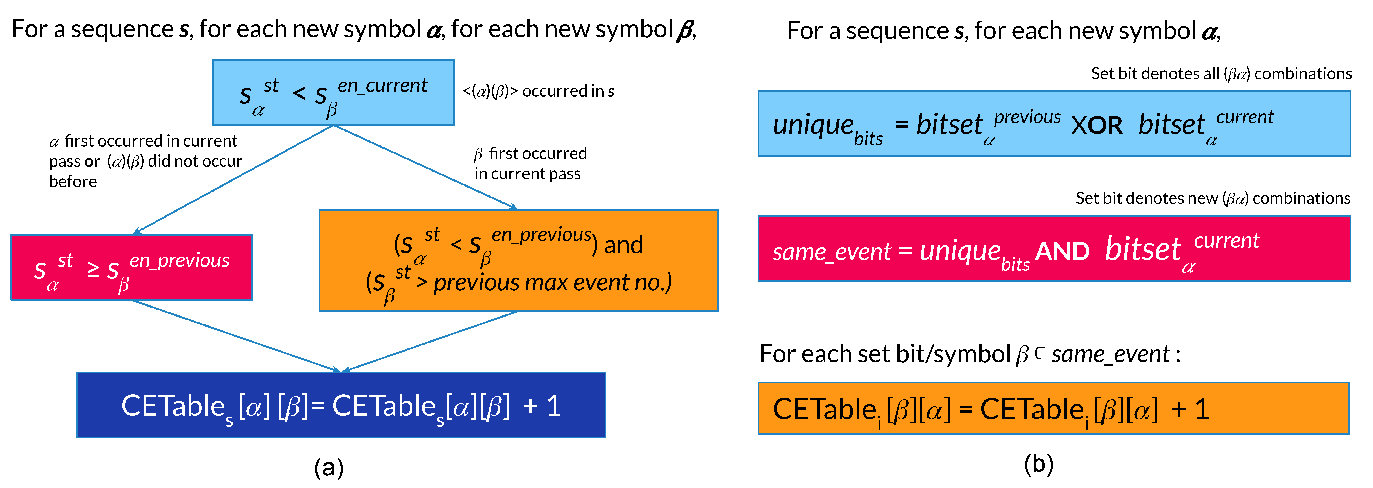
\includegraphics[width=0.5\textwidth]{CETable_calculation}
\caption{(a) $CETable_{s}$ Calculation, (b) $CETable_{i}$ Calculation} \label{figure:cetable_calculation}
\end{figure}

\subsubsection{Pseudocode for Tree Construction}

\begin{algorithm}[!t]
    \small %\small, \footnotesize, \scriptsize, or \tiny
    \caption{Insert sequence into IncSP-Tree}\label{algorithm:insert}
    \begin{algorithmic}[1]
        \State \textbf{Variables: }pass $pa$, node $N$, sequence $s$, previous maximum event $ev_{p}$, running bitset $bit$ to update for each $N$, Item no $I_{no}$, Event No $ev$, Actual event no $ev^{\prime}$.
        \State \textbf{Globals: }$pa$, $s$, $ev^{\prime}$, $seq\_sum$
        \State \textbf{Additional functions: }$len(s)$ returns the number of event in $s$ and $len(s[ev])$ denotes the number of items in event $ev$ of $s$.
        \State \textbf{Output: }$s$ inserted, last node returned, $seq\_sum$ updated.
        \Procedure{InsIncSPTree}{$N, ev, I_{no}, bit$}
            \If{$ev = \text{len}(s)$} \Comment{All events been inserted}
                \State  \text{ Return }$N$
            \EndIf
            \If{($I_{no} > \text{len}(s[ev])$)} \Comment{Add next event}
                \State \Comment{0 Based Indexing}
                \State \text{Return} InsIncSPTree($N$,$ev+1$,0,0)
            \EndIf
            \State $I \gets s[ev][I_{no}]$, $ev^{\prime}=ev+ev_{p}$
            \If{($N.ch[\{I,ev^{\prime}\}] =\{\}$)} \Comment{No child found}
                \State \Comment{create a child node $n$ and initialize the attributes}
                \State $n.I \gets I$, $n.ev \gets ev^{\prime}$, $n.cr \gets pa$, $n.C \gets 0$, $n.C^{\prime} \gets 0$, $n.p_{inf} \gets bit$
                \State $n.md \gets 0$ \Comment{$md$ will be set as $pa$ in Algorithm \ref{algorithm:update_inc_sp}}
                \State $N.ch[\{I,ev^{\prime}\}] \gets n$ \Comment{Setting $n$ as child node}
            \EndIf
            \State $n\gets N.ch[\{I,ev^{\prime}\}]$
            \If{$seq\_sum[s_{sid}][I] = \{\}$}
            \State \Comment{Positional Info update}
            \State $seq\_sum[s_{sid}][I]_{st} \gets ev^{\prime}$,
            \State $seq\_sum[s_{sid}][I]_{en\_previous} \gets ev^{\prime}$
                \State $seq\_sum[s_{sid}][I]_{en\_current} \gets  ev^{\prime}$
            \Else  \Comment{Ending position update}
            \State $\text{ }seq\_sum[s_{sid}][I]_{en\_current}\gets ev^{\prime}$
            \EndIf
            \State \Comment{set bit/items are in same event}
            \State $bit^{\prime} \gets seq\_sum[s_{sid}][I]_{bitset_{current}}$\textbf{ OR }$bit$
            \State $seq\_sum[s_{sid}][I]_{bitset_{current}}\gets bit^{\prime}$ \Comment{Same Event Info update)}
            \State \text{ Return } InsIncSPTree($n$,$ev^{\prime}$,$I_{no}+1,bit^{\prime}$\textbf{ OR }$bit$)
                \State \Comment{$bit^{\prime}$\textbf{ OR }$bit$: Setting bit for $I$ for next call}
        \EndProcedure
    \end{algorithmic}
\end{algorithm}


\begin{algorithm}[!tb]
     \scriptsize %\small, \footnotesize, \scriptsize, or \tiny
    \caption{Updating Attributes of IncSP-Tree} \label{algorithm:update_inc_sp}
    \begin{algorithmic}[1]
        \State \textbf{Globals: }Pass $pa$, list containing nodes for next links and modified next links as $L_{nl}$ and $L_{nl_{m}}$ respectively, Operation type as $t$, list containing underlying $S^{MAL}$ information $L_{S^{MAL}}$.
        \State \textbf{Output: }Update of the concerned branch's attributes.
        \Procedure{Update Path}{$N$}
            \If{($N$ is \textbf{None})}
            \State Return \Comment{All the node's attributes are updated}
            \EndIf
            \State $md^{\prime} \gets N.md$
            \If{$N.md<pa$} $N.md \gets pa$ \Comment{newly modified node}
             \State \Comment{Support Tracking, Runtime memory clear}
                \State $N.C^{\prime} \gets N.C$, $N.nl_{m} \gets \{\}$
            \EndIf
            \For{item $i \in L_{nl_{m}}$}
                    \State \Comment{Tracking underlying modified nodes}
                    \State $N.nl_{m}[i] \gets N.nl_{m}[i] \cup L_{nl_{m}}[i]$
            \EndFor
            \For{item $i \in L_{S^{MAL}}$}
            \State $N.S^{MAL}[i] \gets N.S^{MAL}[i]+1$ \Comment{to reduce loop}
            \EndFor
            \If{$md^{\prime} \neq N.md$} \Comment{$N$ was not tracked}
                \State $L_{nl_{m}}[N.I] \gets N$ \Comment{Need to track $N$ from ancestors for $I$}
            \Else \text{ Delete }$L_{nl_{m}}[N.I]$ \Comment{Already Been Tracked}
            \EndIf
            \If{$t=Insert$}
            \State $N.c \gets N.c+1$,$L_{S^{MAL}} \gets L_{S^{MAL}} \cup \{N.I\}$
            \Else \Comment{ Append Operation}
                \If{$N$ is newly considered node for $s$}
                    \State $N.c \gets N.c+1,L_{S^{MAL}} \gets L_{S^{MAL}} \cup \{N.I\}$
                \Else \Comment{Old nodes, Already Tracked}
                    \State \text{ }$L_{S^{MAL}} \gets L_{S^{MAL}} - \{N.I\}$
                \EndIf
            \EndIf
            \For{item $i \in L_{nl}$} \Comment{Underlying $nl$ update}
            \State $N.nl[i] \gets N.nl[i] \cup L_{nl}[i]$
            \EndFor
            \If{$N.cr = pa$} \Comment{Tracking new nodes for next link}
                \If{$md^{\prime} = N.md$} \Comment{Already Tracked for next link}
                    \State \text{ Delete }$L_{nl}[n.I]$
                \Else $\text{ }L_{nl}[N.I] \gets N$ \Comment{Tracking node for $nl$}
                \EndIf
            \Else \text{ Delete}$L_{nl}[N.I]$ \Comment{Already Tracked by ancestors}
            \EndIf
            \State UpdatePath($N.parent)$
        \EndProcedure
    \end{algorithmic}
\end{algorithm}

As up to now we have talked about the tree attributes and Sequence Summarizer, now we will provide the algorithm to construct these structures from the sequences. The construction method of SP-Tree and IncSP-Tree are similar except IncSP-Tree has some additional attributes. In Algorithm \ref{algorithm:insert}, we provide the pseudo-code to insert a sequence into the tree along with the update of corresponding (track with $sid$) sequence summarizer ($seq\_sum$) based on the input sequence ($s$) and in Algorithm \ref{algorithm:update_inc_sp}, we provide the pseudo-code to update the attributes of the concerned branch of the tree related to the sequence.

For compactness and operational efficiency issues, we have used bitset representation for saving item information, but other representations will also work. The newly used variables are initially provided in the first two lines of the Algorithm \ref{algorithm:insert}. In $Append$ operation, a prefix of the corresponding sequence ($s_{sid}$) already exists and $ev_{p}$ is used to denote that previous maximum event no. In $Insert$ operation, it is considered as $-1$. In Line 11, the actual item ($I$) and event no ($ev^{\prime}$) is calculated. When a desired child node is not found it is calculated and set (line 12-16). $seq\_sum$ is updated in line 18-27. Bit based operations are performed to update Same Event Info of $seq\_sum$ in line 26-27. Finally recursion is called to insert the remaining items in line 28 with child node $n$. Recursion stopping conditions are given in line 6.

Using Algorithm \ref{algorithm:update_inc_sp}, we update the attributes of the tree. As SP-Tree has a subset of attributes from IncSP-Tree, it can follow the same procedure. But whereas IncSP-Tree needs to run it after each sequence insertion, SP-Tree can run only once after complete insertion of the database. Using bottom up recursive traversal with the usage of last node reference of $seq\_sum$ for each sequence $s$ the nodes' attributes are calculated (line 35). For each $N$, its $nl$, $nl_{m}$ and $S^{MAL}$ attributes are updated using the information sent from underlying nodes in lines (25-26), (10-12) and (13-14) respectively. Also, for $N$ the corresponding global lists $L_{nl}, L_{nl_{m}}$ and $L_{S^{MAL}}$ are updated to send its information to its ancestor nodes in lines (27-30), (15-17), (21-24) respectively. In $Insert$ operation, all the nodes' concerning $s$ count attributes are incremented (lines 18-19) whereas in $Append$ operation only the newly considered nodes' for $s$ count attributes get incremented (lines 21-22). In  Algorithm \ref{algorithm:update_inc_sp}, it has been assumed that the mine operation is performed after each batch of data increment. But the proposed framework has no such dependency and can be slightly tweaked to mine anytime based on users' requests.






% An example of a double column floating figure using two subfigures.
% (The subfig.sty package must be loaded for this to work.)
% The subfigure \label commands are set within each subfloat command,
% and the \label for the overall figure must come after \caption.
% \hfil is used as a separator to get equal spacing.
% Watch out that the combined width of all the subfigures on a
% line do not exceed the text width or a line break will occur.
%





%
% Note that often IEEE papers with subfigures do not employ subfigure
% captions (using the optional argument to \subfloat[]), but instead will
% reference/describe all of them (a), (b), etc., within the main caption.
% Be aware that for subfig.sty to generate the (a), (b), etc., subfigure
% labels, the optional argument to \subfloat must be present. If a
% subcaption is not desired, just leave its contents blank,
% e.g., \subfloat[].

\subsubsection{SP-Tree and IncSP-Tree: Visualization}


\begin{figure*}[!htb]
\centering
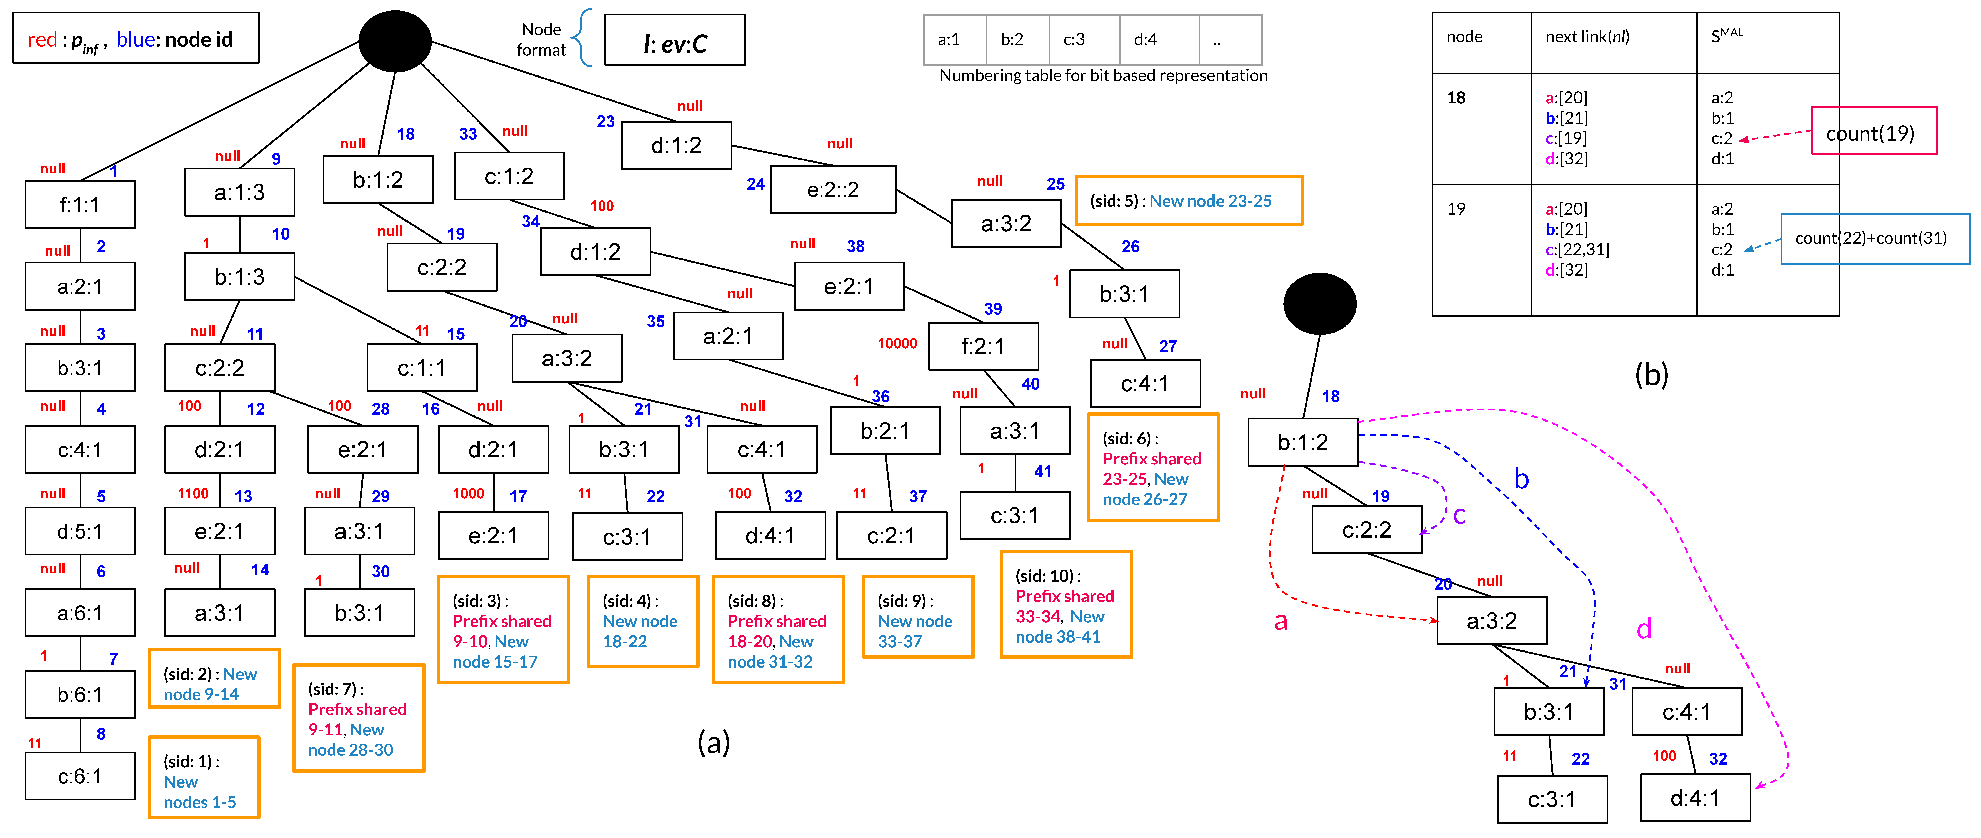
\includegraphics[width=\textwidth]{Complete_SP_Tree_with_next_link}
\caption{(a) Complete SP-Tree, (b) Next links for node 18 and 19} \label{figure:complete_sp_Tree_with_next_link}
\end{figure*}


\begin{figure*}[!htb]
\centering
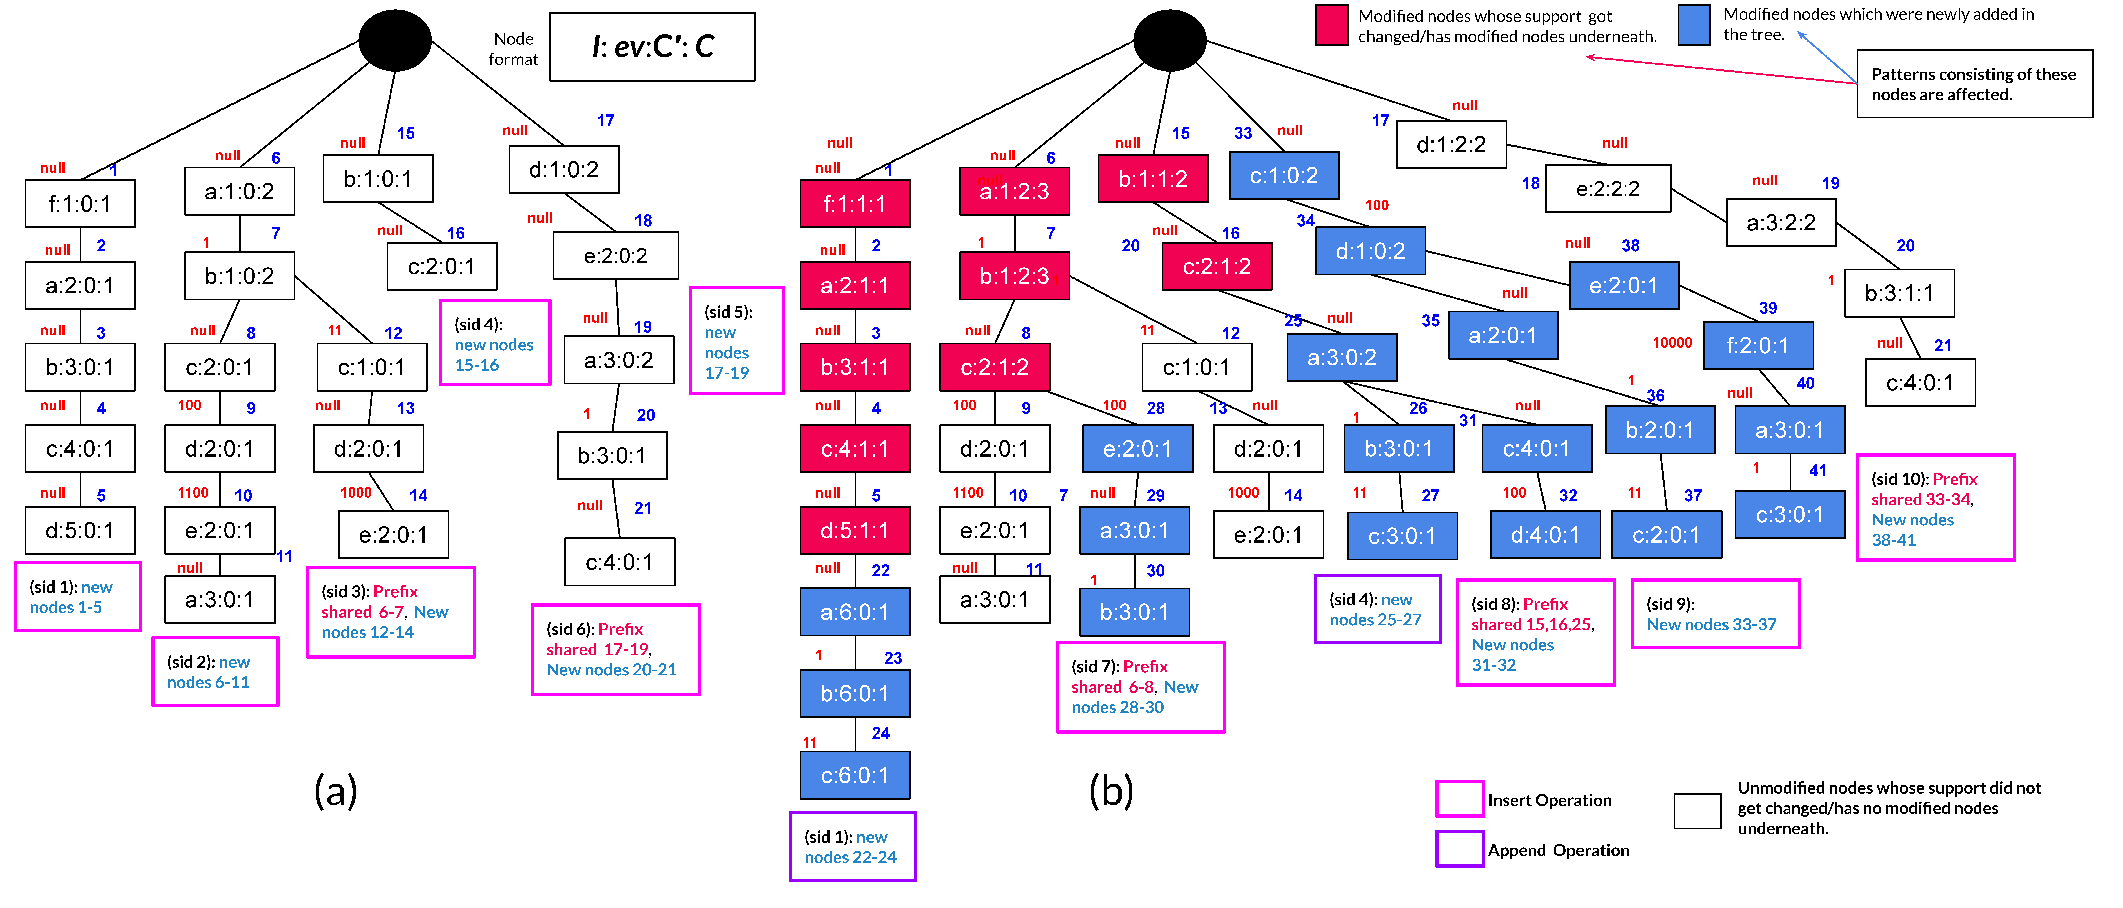
\includegraphics[width=\textwidth]{Complete_IncSP_Tree_with_next_link}
\caption{(a) IncSP-Tree after iteration 1, (b)IncSP-Tree after iteration 2} \label{figure:complete_inc_sp_Tree_with_with_two_pass}
\end{figure*}

In Fig. \ref{figure:complete_sp_Tree_with_next_link} (a), the complete SP-Tree has been shown after inserting all the sequences of the static database into the tree. For simplicity and discussion purpose, it has been assumed that the sequences are inserted according to the increasing order of the sids. Nodes are numbered (blue color) to depict their creation order. In Fig. \ref{figure:complete_sp_Tree_with_next_link}, the complete commentary has been stated to understand how each sequence is inserted, new nodes are created or existing nodes get prefix shared, etc. E.g., due to the insertion of $sid=2$ nodes 9-14 are created and for $sid=3$, nodes 9-10 get prefix shared and nodes 15-17 get newly created. To represent $p_{inf}$ for each node (shown in red color), bit based representation is used and the corresponding numbering scheme has also been shown. For each node, only a single count attribute is used as per the discussion stated in \ref{section:node_attribute}.


In Fig. \ref{figure:complete_inc_sp_Tree_with_with_two_pass}, the proposed IncSP-Tree has been shown for the exampled incremental database for the two iterations. Similar to static mining, sequences are inserted according to the increasing order of $sid$s and nodes' numbers (blue color) depict their creation order. As per the attributes' discussion, for each node two count related attributes have been shown. Inside each node, we have shown four attributes, $I,ev,C^{\prime}$ and $C$ respectively. Before updating an existing branch, first we update the previous count with the present to track the support change between two iterations. Then we perform update where in $Insert$ operation every node's count increases but in $Append$ operation only the nodes which were newly considered due to the new items' arrival in the sequence get incremented. For example nodes (20-22) get incremented but nodes (1-5) do not get incremented after the 2nd pass. This is an $Append$ operation over $sid=1$.

In Fig. \ref{figure:inc_tree_miner_additional_image} (b), we have shown the next links($nl$) and modified next links($nl_{m}$) for node $6$ and $7$ where $nl_{m} \subseteq nl$. This separation is useful to faster traverse in the modified subtrees of IncSP-Tree. When a subtree is modified the corresponding path up to the root is also considered modified so that the ancestor nodes can detect the update in the successor nodes through modified links and count attributes' variation. There are basically two types of modified nodes, those nodes where are newly created (filled in blue color) and those old nodes which (filled in red color) have modified nodes underneath. Uncolored nodes are the unmodified nodes. Patterns consist of the modified nodes are actually the affected patterns due to database increment. In Fig. \ref{figure:static_mining_merged_images} (c) we have shown the sequence summarizer for $sid=1$ after both iterations.


\begin{figure*}[!tb]
\centering
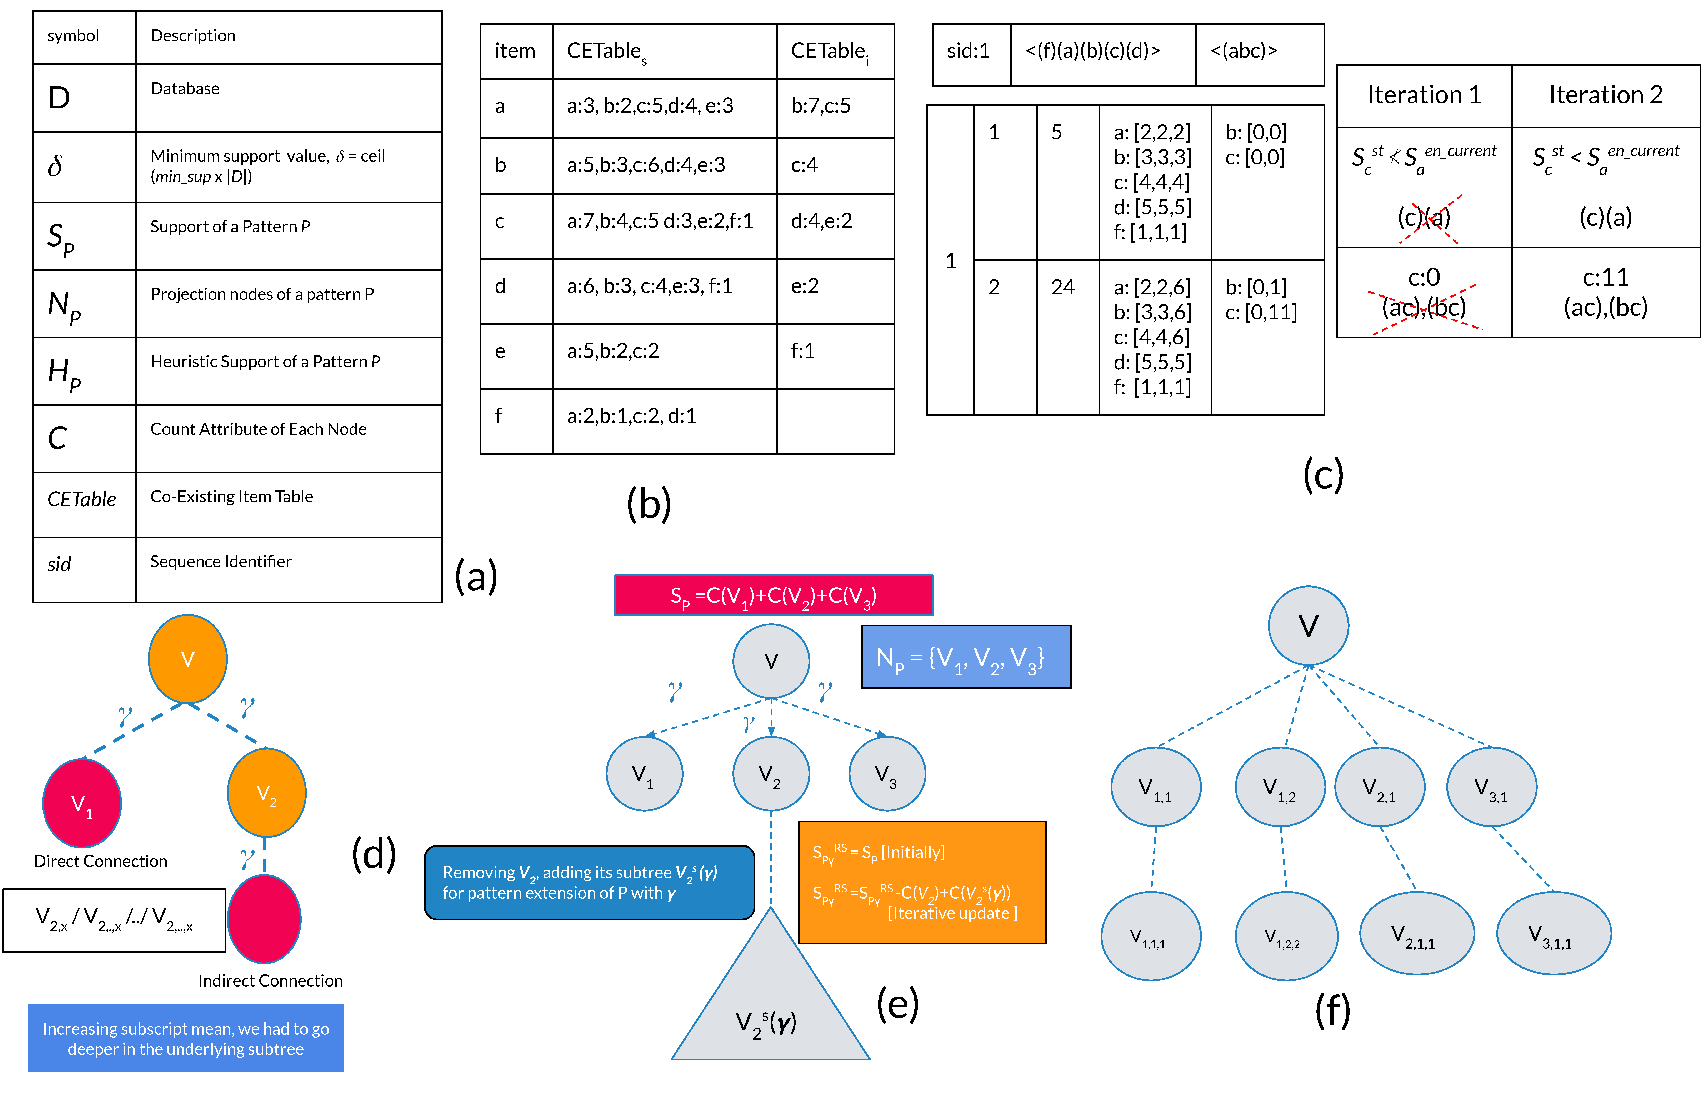
\includegraphics[width=\textwidth]{static_mining_merge_image}
\caption{(a) Terminologies for static mining (b) Co-Existing Item Table, (c) Example of sequence summarizer structure for $sid=1$, (d) Pattern Generation Example, (e) Breadth-First based support counting Technique, (f) Pattern Formation Concepts} \label{figure:static_mining_merged_images}
%\subfloat{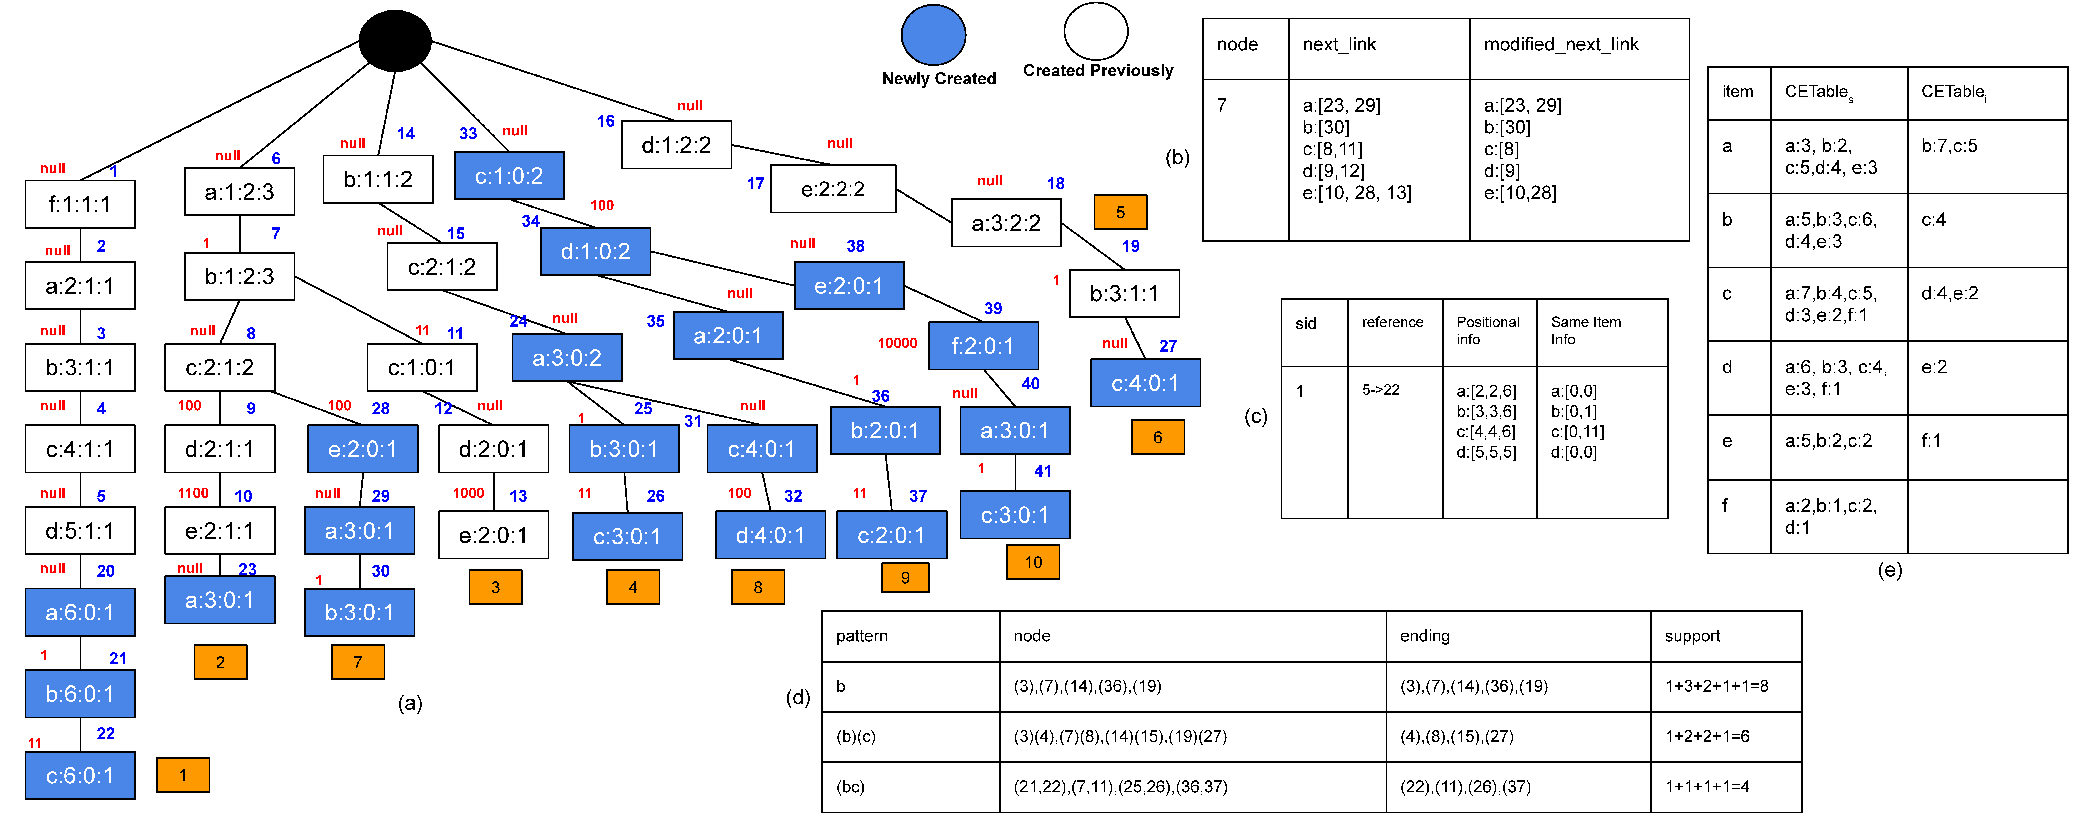
\includegraphics[width=0.70\textwidth]{IncSP-Tree.pdf}
%\label{fig_first_case}}
\hfil
\end{figure*}

\subsection{Pattern Generation from SP-Tree Structures}
Our pattern mining approach follows the pattern growth technique with suffix extension. In the literature mainly two types of pattern extensions are conducted, \textit{Sequence Extension (SE)} means adding a new item as an event in the current pattern and \textit{Itemset Extension (IE)} means adding a new item in the last event of the pattern where the added item is lexicographically (or based on some ordering scheme) larger compared to the existing items of the concerned event.
\begin{definition}[Pattern Formation] \label{defintion:pattern_formation}
     Based on the Fig. \ref{figure:static_mining_merged_images} (f), pattern formation concepts can be pointed as follows -
    \begin{itemize}
        \item Patterns are generated through SP-Tree node concatenations,
i.e., $N_{P}^{\prime}=\{$ $(V, V_{1,1}$, $V_{1,1,1}$), ($V, V_{1,2}$, $V_{1,2,2}$),  ($V$, $V_{2,1}$, $V_{2,1,1}$), ($V$, $V_{3,1}$, $V_{3,1,1}$)$\}$.
    \item Each node concatenation $n  \in  N_{P}^{\prime}$ -
        \begin{enumerate}
            \item Represents a pattern occurrence in a subtree.
            \item Ends in different disjoint subtrees compared to other $n_{j}  \in N_{P}^{\prime}$.
            \item Always the first occurrences in different subtrees are considered.
        \end{enumerate}
         So, a pattern $P$ can be represented by the nodes where it ends,  $N_{P}$=$\{$ $V_{1,1,1}$,  $V_{1,2,2}$,  $V_{2,1,1}$,   $V_{3,1,1}\}$.
    \item Support of $P$ is $S_{P}$ =  $\sum_{n \in N_{P}} C(n)$. $C$ denotes the count attribute of each node.
    \item For each $n \in N_{P}$ , we can say that, we have completed searching up to that node. During following iterations, we will search only in their underlying subtrees.
    \end{itemize}
\end{definition}

In Fig. \ref{figure:pattern_extension_example}, we have shown an example of pattern formation which states how the nodes' concatenation can form a pattern and for each occurrence the last node position can represent the pattern in a subtree.

Suppose, we have a pattern $P=< (\alpha\beta) >$ ending at nodes $N_{P}=\{V_{i},V_{j},V_{k},..,V_{n}\}$. We want to find nodes $N_{P\gamma}$ which will extend $P$ for $\gamma$. For each $V \in N_{P}$, we follow similar extension procedure ($SE/IE$) each having two cases. Based on Fig. \ref{figure:static_mining_merged_images} (d), we can discuss the extensions as follows -

\begin{definition}[SE in SP-Tree, $P \,\to\, P\{\gamma\}$]
Two cases are -
\begin{enumerate}
    \item Direct Connection: For a node $V \in N_{P}$ suppose through next link for $\gamma$, we reach node $V_{1}$($V.nl[\gamma]=\{V_{1}\}$). If $V.ev \neq V_{1}.ev$, then $V_{1}$ can perform SE over $V$. E.g., $(a)\,\to\,(a)(b)$ with nodes $\{(2)\,\to\,(3)\}$ (Fig. \ref{figure:pattern_extension_example}).
    \item Indirect Connection:  For a node $V \in N_{P}$ suppose through next link for $\gamma$, we reach node $V_{2}$($V.nl[\gamma]=\{V_{2}\}$). If $V.ev = V_{2}.ev$ then $V_{2}$ can not perform SE over $V$. Then, we need to search in underlying subtree of $V_{2}$ to find such node(s) $V_{2,...,x}$ where $V.ev \neq V_{2,...,x}.ev$. In this case, we need to perform two level next link traversals for $\gamma$ from $V$. E.g., $(a)\,\to\,(a)(b)$ with nodes $\{(6)\,\to\,(7)\,\to\,(30)\}$ (Fig. \ref{figure:pattern_extension_example}).
\end{enumerate}
\end{definition}


\begin{definition}[IE in SP-Tree,  $P \,\to\, \{P\gamma\}$]
Two cases are -
\begin{enumerate}
    \item Direct Connection:  For a node $V \in N_{P}$ suppose through next link for $\gamma$, we reach node $V_{1}$. If $V.ev = V_{1}.ev$, then $V_{1}$ can perform IE over $V$. E.g., $(a)\,\to\,(ab)$ with nodes $\{(6)\,\to\,(7)\}$ (Fig. \ref{figure:pattern_extension_example}).
    \item Indirect Connection:  For a node $V \in N_{P}$ suppose through next link for $\gamma$, we reach node $V_{2}$.  If $V.ev \neq V_{2}.ev$ then $V_{2}$ can not perform IE over $V$. Then, we need to search in underlying subtree of $V_{2}$ to find such node(s) $V_{2,...,x}$ which have items $\alpha$,$\beta$ in the same event as it found in its predecessor nodes. From a node's $p_{inf}$ we get the items which are in the same event as it and can be calculated through bitwise AND operation. E.g., $(a)\,\to\,(ab)$ with nodes $\{(2)\,\to\,(3)\,\to\,(21)\}$ (Fig. \ref{figure:pattern_extension_example}).
\end{enumerate}
\end{definition}

To search in a node's underlying subtree we take all the nodes reached through next link and simulate each connection cases. In Fig. \ref{figure:complete_sp_Tree_with_next_link} (b), we have shown a small visualization of traversing through next links. Our node extension procedure works in level by level manner through our proposed breadth-first based support counting mechanism.

\begin{figure*}[!tb]
\centering
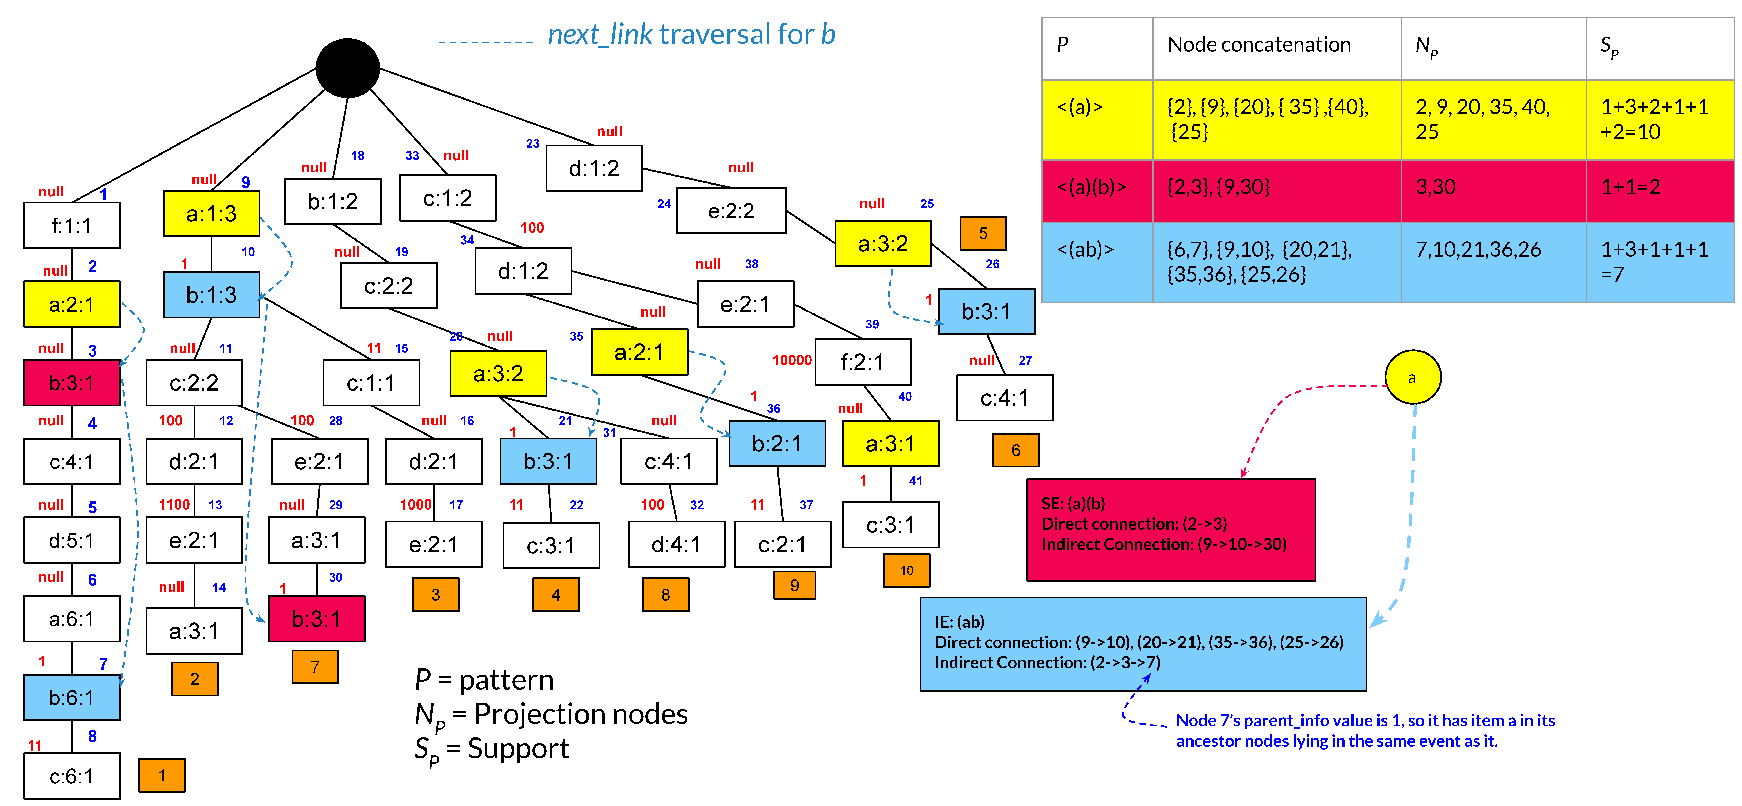
\includegraphics[width=\textwidth]{pattern_extension_example}
\caption{Pattern Extension Examples} \label{figure:pattern_extension_example}
\hfil
\end{figure*}


\subsection{Pruning Techniques}
In this section, we will discuss the applied pruning techniques that help to detect the redundant patterns early and reduce the search space. Suppose, we have a pattern $P=< (\alpha\beta) >$ with support $S_{P}$ ending at nodes $N_{P}=\{n_{1},n_{2},n_{3},...,n_{k}\}$ and corresponding $sList=\{\alpha,\beta,\gamma,\delta\}$ and $iList=\{\gamma,\delta\}$. $sList$ and $iList$ give idea regarding which items may extend $P$ as SE and IE respectively. Let $\delta= \ceil{min\_sup \times \vert D \vert}$. First, we will discuss the support downward closure. The terminologies used in static mining discussion has been shown in Fig. \ref{figure:static_mining_merged_images}(a).

% https://tex.stackexchange.com/questions/215763/dot-missing-after-the-number-of-section-when-using-llncs-cls
\begin{lem}[Support Downward Closure] \label{lem:support_constraint}
    From a node $n_{i} \in N_{P}$, suppose we reach a set of nodes $M=\{m_{1,i},m_{2,i},...,m_{x,i}\}$ through next link for any item $\epsilon$, where each $m \in M$ are in disjoint subtrees and $m_{j,i}$ denotes the $j^{th}$ branch in $n_{i}$'s subtree. Then $C(n_{i}) \geq  \sum_{j=1}^{x} C(m_{j,i})$.
\end{lem}
\begin{proof}
    This holds because of the tree's node overlapping characteristics.
\end{proof}
Now, we will discuss the pruning strategies based on their execution order.
\subsubsection{CETable Based Pruning}
First, we will provide the definition of this strategy stated in a lemma. Following that, we will give some examples to understand it.
\begin{lem}[CETable Based Pruning] \label{lem:cetable}
   An item $\gamma$ can extend $P$ as sequence extension iff $CETable_{s}[\alpha][\gamma] \geq \delta$ and $CETable_{s}[\beta][\gamma] \geq \delta$. Similarly $\gamma(\gamma > \beta > \alpha)$ can extend $P$ as itemset extension  $CETable_{i}[\alpha][\gamma] \geq \delta$ and $CETable_{i}[\beta][\gamma] \geq \delta$. For each item $I$ belongs to last event of $P$ this constraint is checked.
\end{lem}
\begin{proof}
    CETable holds the co-occurrence information of the items and for any super pattern to satisfy $min\_sup$ constraint, its sub patterns also need to satisfy. This was adopted in our solution from \cite{fournier2014fast}.
\end{proof}

For example, suppose, $\delta=3$, now pattern $< (a)(c)(b) >$ can not be frequent, because $<(a)(b) >$ is not frequent (in $CETable_{s}$ column of Fig. \ref{figure:static_mining_merged_images}(b), $S_{(a)(b)}=2 < \delta$). Similar pruning strategy can also be applied based on $CETable_{i}$ column.

\subsubsection{Breadth-First Based Support Counting Technique}

Now, we will talk about our proposed new \textit{Breadth-First Based Support Counting Technique} which is stated in Algorithm \ref{algorithm:breadth_first_support}. We have used comment to understand the underlying logic behind the statements. This technique is valid because of the Lemma \ref{lem:support_constraint}. When we remove a node and go deeper in the subtree the maximum possible support for the extended pattern will stay same or reduce. Theoretically the strategy is explained in Lemma \ref{lem:bfs_prune} using Fig. \ref{figure:static_mining_merged_images} (e).

\begin{algorithm}[!t]
           \scriptsize %\small, \footnotesize, \scriptsize, or \tiny
            \caption{Breadth-First Based Support Counting}
            \label{algorithm:breadth_first_support}
        \begin{algorithmic}[1]
            \State \textbf{Globals: }$\delta = min\_sup \times \vert D \vert$
            \Procedure{BreadthFirstSupportCounting}{$P,N_{P},\gamma, S_{P}$}
                \State \Comment{Extended Nodes, Actual Support,Queue}
                \State $N_{P\gamma} \gets \{\},S^{RS}_{P\gamma} \gets S_{P},Q \gets N_{P}$
                 \For{each node $n_{i} \in Q$}
                 \State \Comment{Extending $P$ for $\gamma(P\gamma):(\alpha\beta)(\gamma)\text{ or }(\alpha\beta\gamma)$}
                    \If{($S^{RS}_{P\gamma}-C(n_{i})+n_{i}.S^{MAL}[\gamma] < \delta$)}
                    \State Return Infrequent
                    \EndIf
                    \State \Comment{Removing Node, Will check in subtree}
                    \State $Q \gets Q - \{n_{i}\}$ , $S^{RS}_{P\gamma} \gets S^{RS}_{P\gamma}-C(n_{i})$
                    \For{each node $m_{j}\in n_{i}.nl[\gamma]$}
                        \State \Comment{Maximum possible support can be found in $S^{RS}_{P\gamma}$}
                        \State $S^{RS}_{P\gamma} \gets S^{RS}_{P\gamma}+C(m_{j})$
                        \If{(pattern extension constraint satisfied)}
                            \State $N_{P\gamma} \gets  N_{P\gamma} \cup m_{j}$
                        \Else  \Comment{Need to check further in underlying subtrees}
                            \State $Q \gets Q \cup \{m_{j}\}$
                        \EndIf
                    \EndFor
                    \If{($S^{RS}_{P\gamma} < \delta$)} Return Infrequent
                    \EndIf
                \EndFor
                \State Return $N_{P\gamma},S^{RS}_{P\gamma}$ \Comment{Frequent: Return extension nodes with actual support}
            \EndProcedure
        \end{algorithmic}
    \end{algorithm}

\begin{figure*}[!t]
\centering
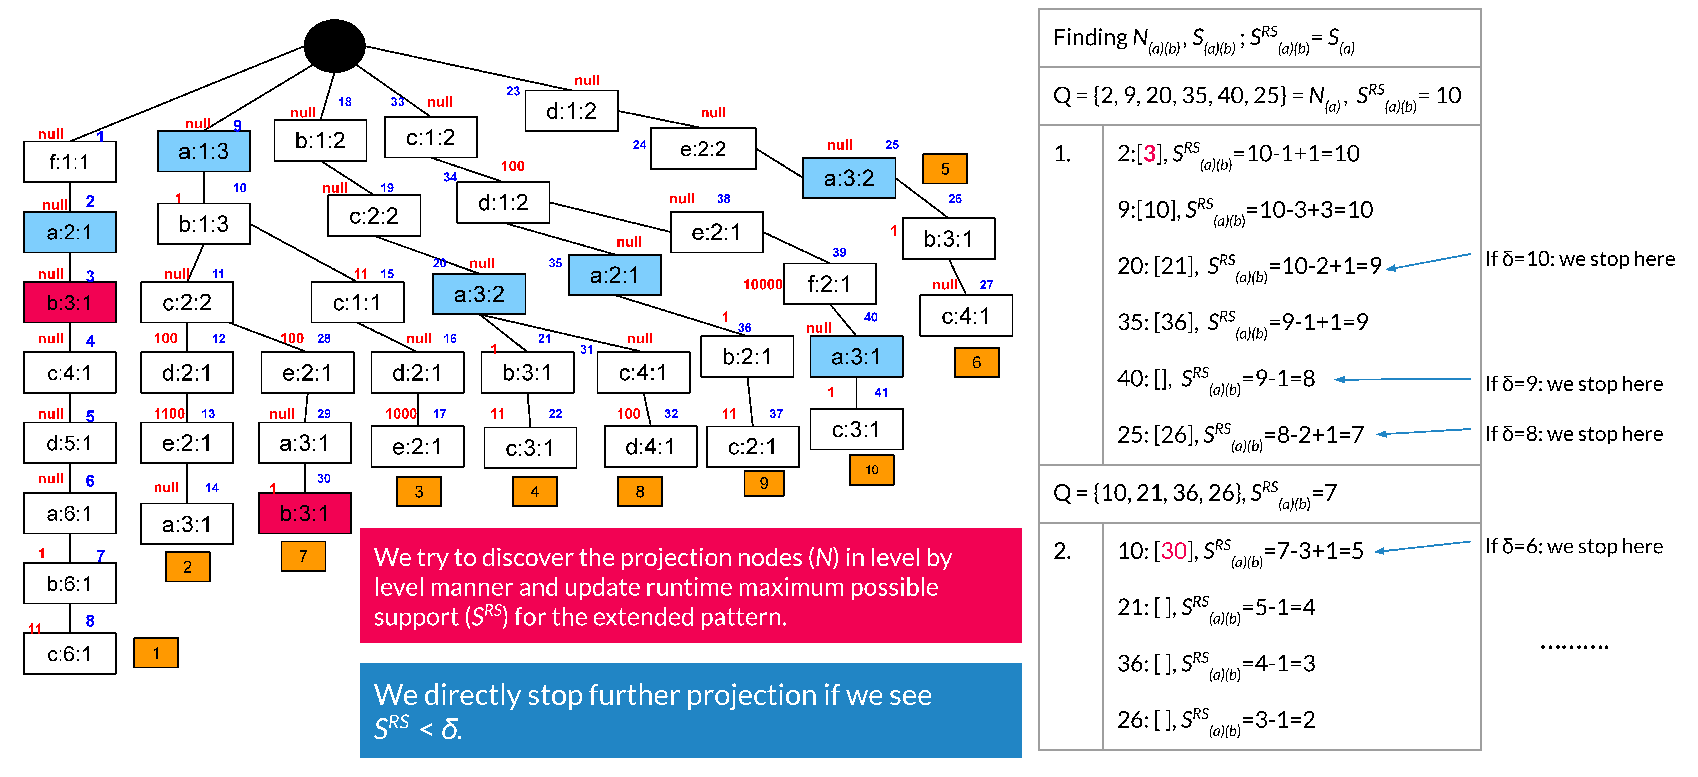
\includegraphics[width=\textwidth]{Example-Breadth-First-Support}
\caption{Simulation of Breadth-First Based Support Counting Technique} \label{figure:breadth_first_technique_example}
\hfil
\end{figure*}

\begin{lem}[Breadth-First Based Counting Strategy]\label{lem:bfs_prune}
  Suppose, from a pattern $P$ we have to check extension for $P\gamma$ from a set of projection nodes, $N_{P}=\{V_{1},V_{2},V_{3}\}$ where initially current maximum possible support for the extended pattern is $S_{P\gamma}^{RS}=S_{P}$. For each $n \in N_{P}$, it is removed, its underlying subtree($n^{s}(\gamma)$) is added for iterative searching and the runtime maximum possible support gets updated to $S^{RS}_{P\gamma}=S_{P}^{RS}-C(n)+\sum C(n^{s}(\gamma))$. The extension nodes for $N_{P\gamma}$ is discovered in level by level manner.
\end{lem}

\begin{proof}
     As, $C(V) \geq \sum C(V_{2}^{s}(\gamma))$ [Lemma \ref{lem:support_constraint}], so $S^{RS}_{P\gamma} \leq S_{P}$.
\end{proof}


The main advantage of this technique is, we may detect the infrequency of a pattern early without performing its complete projection. A small simulation to understand this technique has been shown in Fig \ref{figure:breadth_first_technique_example}. In Fig. \ref{figure:breadth_first_technique_example} we have shown how we will calculate the projection nodes for the pattern $< (a)(b) >$. We discover the nodes in level by level manner and may stop projecting at any time based on the maximum possible support.



\subsubsection{Heuristic $iList$ Pruning} \label{section:heuristic_pruning}
This is our second proposed pruning strategy and stated in Lemma \ref{lem:heu_i_prune}.
\begin{lem}[Heuristic $iList$ Pruning] \label{lem:heu_i_prune}
   Suppose, We have an item $\epsilon(\epsilon \in sList \cap iList)$. During support calculation as SE for $\epsilon$, we collectively reach nodes $M=\{m_{1,1},m_{2,1},..,m_{1,2},m_{2,2},..,m_{1,x},..,m_{2,y},..,m_{k,z}\}$ from $n.nl[\gamma]; \forall n \in N_{P}$. Let $H_{P\{\epsilon\}}= \sum_{m \in M} C(m)$. If heuristic support, $H_{P\{\epsilon\}} <  \delta$, then $\epsilon$ can not pefrorm IE over $P$ and can be removed from $iList$.
\end{lem}
\begin{proof}
    Intuition lies behind Lemma \ref{lem:support_constraint}. Actual support for IE, $S_{\{P\epsilon\}} \leq H_{P\{\epsilon\}} < \delta$. Because we need to go deeper to find the valid nodes for the extension.
\end{proof}

To understand this strategy, an example can be seen using SP-Tree of Fig. \ref{figure:complete_sp_Tree_with_next_link}. Here $N_{(a)}=\{2, 9, 20, 35, 40, 25\}$. For $b$, $< (a) >$ will be extended. Now, the first level nodes reached through next links for $b$ from each $n \in N_{(a)}$ are $\{3, 10, 21, 36, 26\}$ and total heuristic support $H_{(a)(b)}$ is $7$ ($C(3)+C(10)+C(21)+C(36)+C(26)$). Now, if $H_{(a)(b)} < \delta$, then without any further checking $b$ can be removed from both $sList$ and $iList$.

\subsubsection{Recursive $sList$ and $iList$ pruning}
This strategy is stated in Lemma \ref{lem:s_i_prune}. The lemma \ref{lem:s_i_prune} is a very widely addressed pruning strategy which has been adopted in our solution and it comes from the apriori property that if $< (\alpha)(\gamma) >$ is not frequent, then $< (\alpha)(\beta)(\gamma) >$ will never be frequent.

\begin{lem}[Recursive $sList$ and $iList$ pruning ] \label{lem:s_i_prune}
Suppose, after support calculation the found shrinked lists are $sList^{\prime}=\{\alpha,\beta,\gamma\}$ and $iList^{\prime}=\{ \delta \}$ which will extend $P$. Now during recursive extensions for each $\theta \in sList^{\prime}$ as SE the corresponding sList and iList will be $sList^{\prime}$ and $\{\epsilon \vert \epsilon \in sList^{\prime} \cap \epsilon >_{order} \theta\}$ respectively. Similarly to perform IE for each $\theta \in iList^{\prime}$ the corresponding sList and iList will be $sList^{\prime}$ and $\{\epsilon \vert \epsilon \in iList^{\prime} \cap \epsilon >_{order} \theta\}$ respectively.
\end{lem}

\subsubsection{Loop Reduction}
This implementational strategy is also designed using the node properties and theoretically stated in Lemma \ref{lemma:loop_reduction} and applied in Algorithm \ref{algorithm:breadth_first_support}. Before searching for an item in the underlying subtree, first the corresponding value in $S_{MAL}$ is checked and the possible maximum support is heuristically calculated. If this heuristic value fails to support $\delta$, then there's no need to perform more projection.

\begin{lem}[Loop Reduction] \label{lemma:loop_reduction}
Suppose, we want to extend from node $n \in N_{P}$ for an item $\epsilon$ and current maximum possible support for the extended pattern is $S_{P\epsilon}^{RS}$. If, $(S_{P\epsilon}^{RS}-C(n)+n.S^{MAL}[\epsilon]) < \delta$, then $P\epsilon$ can be detected as infrequent.
\end{lem}
\begin{proof}
    For any $P$'s projection node $N_{P}$ for any item $\epsilon$, $N_{P}.S^{MAL}[\epsilon] = \sum_{n \in N_{P}.nl[\epsilon]}C(n) \geq \sum_{n^{\prime} \in N_{P\epsilon}} C(n^{\prime})$.
\end{proof}






\subsection{BPFSP-Tree: Bi-Directional Projection Pointer Based Frequent Sequential Pattern Tree}
In ISPM problem, after each iteration, we need to report the current list of frequent patterns with their support. So, to store the frequent patterns traditional literature maintain a tree-like structure \cite{chen2007incremental,liu2012incremental}. In our study, we propose a new tree-based structure named \textit{Bi-Directional Projection Pointer Based Frequent Sequential Pattern Tree (BPFSP-Tree)} to store the patterns with their support and projections using \textit{IncSP-Tree} node pointers. An important point to note that generally in most of the cases (or after some iterations) the size of the incremental database gets quite smaller compared to the size of the existing database. Thus why, generally after some iterations, a pattern's transition from frequent to infrequent or vise-versa occurs slowly. Moreover, it is the normal characteristic that either an existing frequent pattern's super pattern will get infrequent to frequent or a current frequent pattern along with its some of the sub-patterns will get frequent to infrequent also with the addition of some completely new patterns with new prefix as frequent. So, it is important to give focus on the frequent patterns' representation because they might control the DB scan. The main features and characteristics of our proposed \textit{BPFSP-Tree}($B$) is as follows -
\begin{enumerate}
    \item \textit{Pattern, Support and Projection Pointer: }BPFSP-Tree stores the frequent patterns($P$) with their corresponding support($S_{P}$) and projection nodes($N_{P}$) through prefix sharing. So, for each node $B_{P}$ a frequent pattern($P$) can be formed concatenating the items of the nodes from root($B_{root}$) to it($B_{P}$) in order. $B_{P}$'s support and projection pointers will denote $P$'s support($S_{P}$) and projection nodes($N_{P}$). Projection information reduces the number of DB scans by directly reaching this node and getting the projection info for further extensions ($N_{P} \to N_{P\gamma}$).

    \item \textit{Non-Frequent Item Buffer(NIB): }Suppose during pattern extension for a frequent pattern $P$, $P \to P\gamma$'s projection is completely calculated. Then to mitigate this cost, only $S_{P\gamma}$ is stored in an item buffer in $B_{P}$ to use it in the successive mining iterations by implicitly merging modified and unmodified nodes' support. This buffer is called \textit{Non-Frequent Item Buffer(NIB)}.

    \item \textit{Bottom up pruning using end-link}: After a mining iteration some previously frequent patterns can become infrequent. To remove such patterns from BPFSP-Tree, bottom up strategy is followed which leads to traverse lesser nodes. To traverse from one leaf node to another in BPFSP-Tree, a link is maintained named as $end\_link$.

     A small example of BPFSP-Tree is shown in Fig. \ref{figure:inc_tree_miner_additional_image} (c) with $end\_link$s for traversing through the leaf nodes using SP-Tree node references of Fig. \ref{figure:complete_inc_sp_Tree_with_with_two_pass} (b).
\end{enumerate}

\begin{figure*}[!tb]
\centering
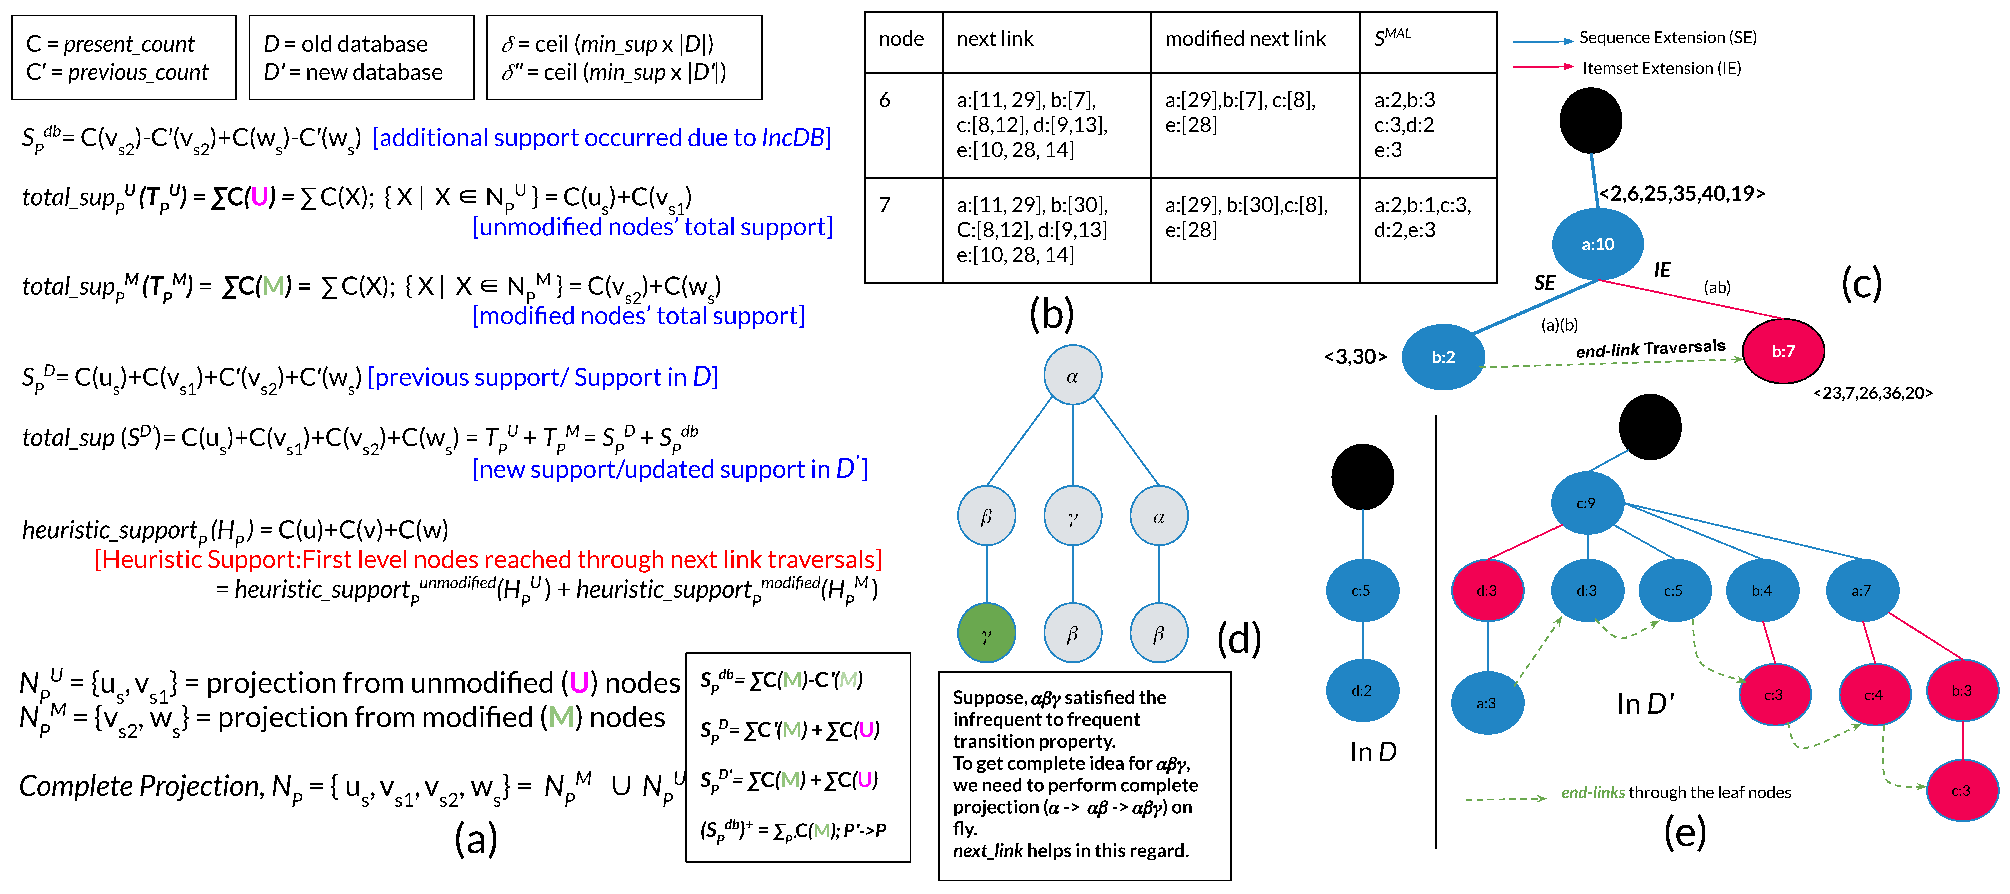
\includegraphics[width=\textwidth]{incremental_mining_merge_im1}
\caption{(a) Pattern Generation Approach for IncTree-Miner, (b) Example of next links and modified next links, (c) Example of BPFSP-Tree, (d) Memory Resilient IncTree-Miner, (e) BPFSP-Tree for patterns with prefix $< c >$ after iteration 1 and 2 for $\delta=2, \delta^{\prime}=3$.} \label{figure:inc_tree_miner_additional_image}
\hfil
\end{figure*}

\subsection{Mining Algorithms}
In this section, based on the above discussions, we will describe our proposed
mining algorithms. Tree-Miner based on SP-Tree and IncTree-Miner based on IncSP-Tree are two algorithms to mine the complete set of frequent patterns for static and incremental database respectively. The main challenge of an incremental mining algorithm is how to efficiently track those patterns which are affected due to the addition of IncDB rather than complete mining. IncTree-Miner is efficiently designed to solve this challenge.

\subsubsection{Tree-Miner: Static Mining Algorithm}
\begin{algorithm}[!t]
    \scriptsize %\small, \footnotesize, \scriptsize, or \tiny
    \caption{Tree-Miner}
    \label{algorithm:tree_miner}
    \begin{algorithmic}[1]
        \State \textbf{Globals: }$\delta=\ceil{min\_sup \times \vert D \vert}$
        \State \textbf{Output: }Complete set($F$) of frequent sequential patterns.
        \Procedure{TreeMiner}{$P,N_{P},sList,iList$}
            \State \Comment{CETable based pruning}
            \State Reduce $sList$ and $iList$ based on CETable.
            \State \Comment{Nodes which will perform extension}
            \State $N_{SE}\gets \{\},N_{IE} \gets \{\}$
            \For{each item $\gamma \in sList$} \Comment{SE checking}
                \State $\forall n \in N_{P}$ perform SE for $\gamma(P\{\gamma\})$
                \If{($S_{P\{\gamma\}} < \delta$)}
                    \State $sList \gets sList -\{\gamma\}$\Comment{Infrequent Pattern}
                    \If{($H_{P\{\gamma\}} < \delta$ and $\gamma \in iList$)}
                        \State $iList \gets iList -\{\gamma\}$ \Comment{\ref{section:heuristic_pruning}}
                    \EndIf
                \Else \Comment{Frequent Pattern, tracking extension nodes}
                    \State $N_{SE}[\gamma] \gets N_{P\{\gamma\}}$
                \EndIf
            \EndFor
             \For{each item $\gamma \in iList$} \Comment{IE checking}
                \State $\forall n \in N_{P}$ perform IE for $\gamma(\{P\gamma\})$
                \If{($S_{\{P\gamma\}} < \delta$)}
                \State $iList \gets iList -\{\gamma\}$\Comment{Infrequent Pattern}
                \Else \Comment{Frequent Pattern, tracking extension nodes}
                    \State $N_{IE}[\gamma] \gets N_{\{P\gamma\}}$
                \EndIf
            \EndFor
            \For{(each item $\gamma \in sList$)} \Comment{Recursive SE}
                \State TreeMiner($P\{\gamma\},N_{SE}[\gamma],sList,\{\alpha \vert \alpha \in sList \cap \alpha > \gamma \}$)
            \EndFor
            \For{(each item $\gamma \in iList$)} \Comment{Recursive IE}
                \State TreeMiner($\{P\gamma\},N_{IE}[\gamma],sList,\{\alpha \vert \alpha \in iList \cap \alpha > \gamma \}$)
            \EndFor
        \EndProcedure
    \end{algorithmic}
\end{algorithm}

Our mining approach is based on forward mining with suffix extension. We start with a single item pattern $P$ with the information in which nodes $N_{P}$ it ends along with two supporting lists, $sList$ and $iList$, which give idea regarding the items which might perform SE and IE over it. To extend $P$ for an item $\gamma$, we find the desired nodes for each $n \in N_{P}$ in the underlying subtrees and recursively perform the extensions with the shrunken $sList$ and $iList$ through our proposed support counting technique and pruning strategies. We have provided the pseudo-code for Tree-Miner in Algorithm \ref{algorithm:tree_miner}. Here, $S_{P}$ and $H_{P}$ denote a pattern $P$'s actual and heuristic support respectively. In Fig. \ref{figure:tree_miner_simulation}, we have shown how patterns are recursively discovered in Tree-Miner. To visualize, we have shown the generated patterns with prefix $< (a) >$ and considered $\delta=2$. For each pattern we have shown its support, its initial $sList$,$iList$, shrinked $sList^{\prime}$, $iList^{\prime}$ and corresponding projection nodes. Node numbers can be mapped to the exampled SP-Tree.



\begin{figure*}[!tb]
\centering
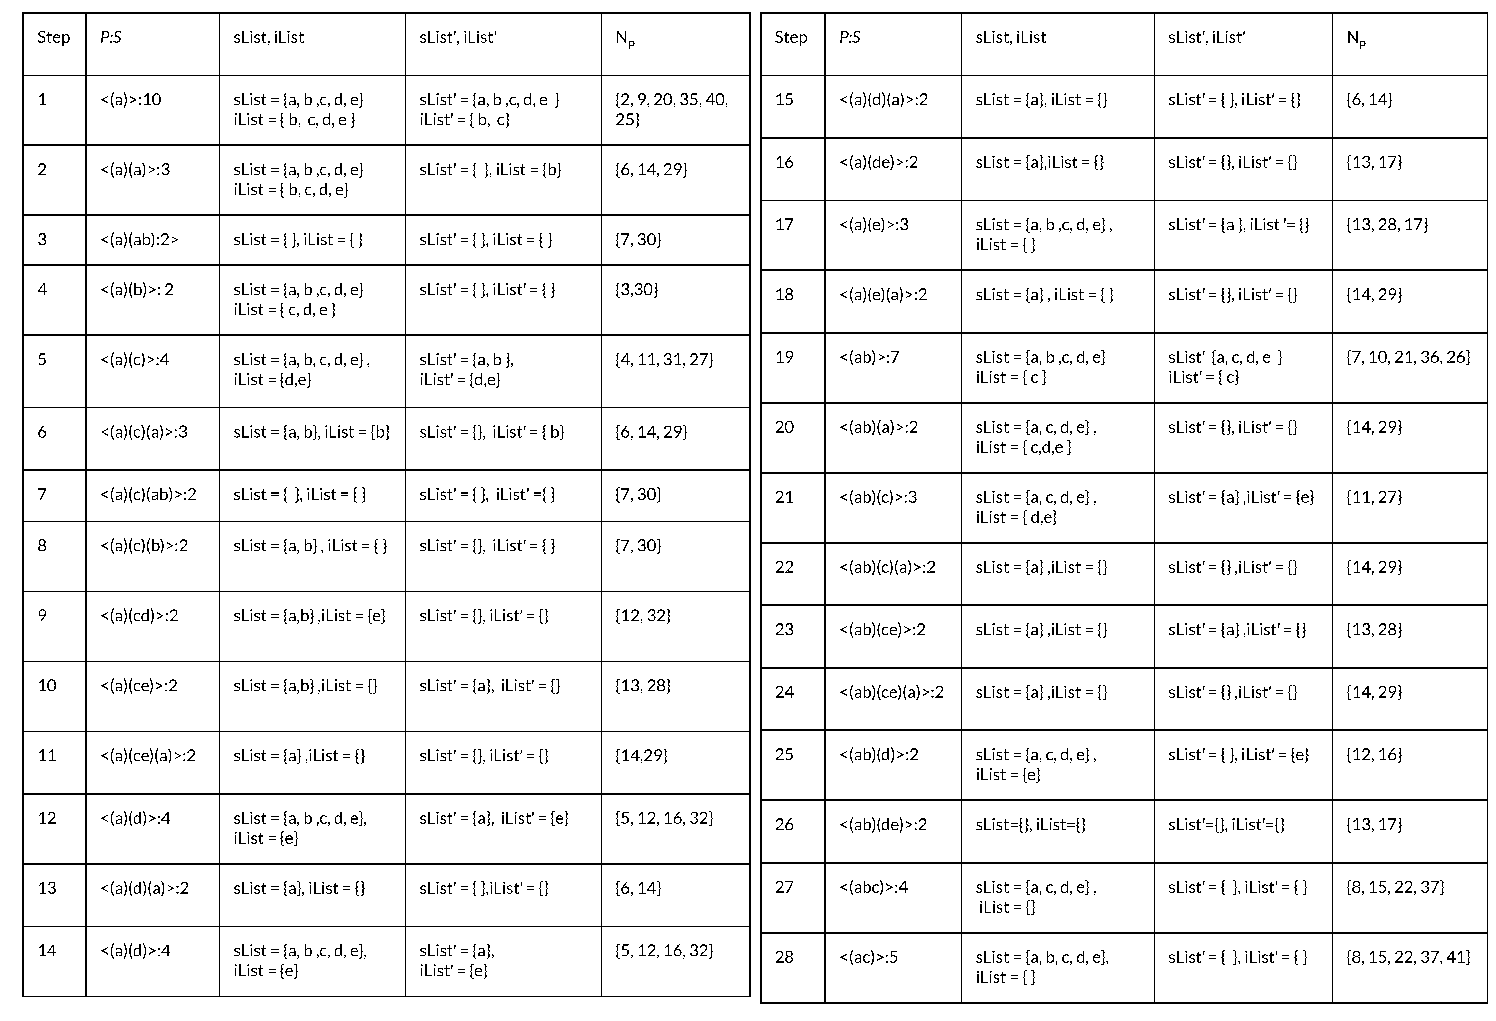
\includegraphics[width=\textwidth]{Tree-Miner-Simulation}
\caption{Simulation of Tree-Miner for the patterns with prefix $< (a) >$} \label{figure:tree_miner_simulation}
\hfil
\end{figure*}

\subsubsection{IncTree-Miner: Incremental Mining Algorithm}


\begin{algorithm}[!thb]
      \scriptsize
      \caption{Pattern Formation Block of IncTree-Miner}
      \label{algorithm:pattern_formation_inctree_miner}
      \begin{algorithmic}[1]
           \Procedure{PatternFormation}{$P\gamma$, $N_{P}^{M}$, $B_{P}$}
           \State \forall $n \in N_{P}^{M}$ perform implicit projection in modified subtrees for $\gamma$
           \State \Comment{previously frequent, $B_{P\gamma}$ node exists}
            \If{$P\gamma \in B_{P}.child$ }
                \If{$S_{P\gamma}^{D^{\prime}} \geq \delta^{\prime}$} update support and projection in $B_{P\gamma}$.
                \Else  \Comment{Got Infrequent}
                    \State Remove $B_{P\gamma}$ and its subtree, adjust end-links.
                    \If{(complete projection done)}
                    \State \Comment{Save support in NIB}
                    \State $B_{P}.NIB[\gamma] \gets S_{P\gamma}^{D^{\prime}}$
                    \EndIf
                \EndIf
            \ElsIf{$\gamma \in B_{P}.NIB$}
                \State \Comment{Previous complete support in NIB}
                \If{$S_{P\gamma}^{D^{\prime}} \geq \delta^{\prime}$}
                    \State Perform projection in unmodified subtrees for $\gamma$.
                    \State Create node $B_{P}.child[\gamma]$, adjust end-links, remove  $B_{P}.NIB[\gamma]$
                \Else \Comment{Still Infrequent}
                    \If{(complete projection done)}
                        \State $B_{P}.NIB[\gamma]\gets S_{P\gamma}^{D^{\prime}}$
                    \Else \Comment{Not full projection calculated}
                        \State \text{ }Delete  $B_{P}.NIB[\gamma]$
                    \EndIf
                \EndIf
            \ElsIf{$P\gamma \notin B_{P}.child \cap \gamma \notin B_{P}.NIB$}
                \If{$S_{P\gamma}^{db} \geq \delta^{\prime}-\delta+1$}
                    \State  \Comment{Infrequent to Frequent Transition}
                    \State Perform projection in unmodified subtrees for $\gamma$.

                    \If{$S_{P\gamma}^{db}+S_{P\gamma}^{D}=S_{P\gamma}^{D^{\prime}} \geq \delta^{\prime}$}
                    \State Create $B_{P}.child[\gamma]$,adjust links
                    \Else \Comment{Infrequent Pattern}
                        \If{(complete projection done)}
                            \State $B_{P}.NIB[\gamma] \gets S_{P\gamma}^{D^{\prime}}$
                        \EndIf
                        \If{$H_{P\gamma}^{M}+H_{P\gamma}^{U} < \delta^{\prime}$}
                            \State \Comment{Heuristic Pruning during SE}
                            \State Remove $\gamma$ from $iList$ of pattern $P$
                        \EndIf
                    \EndIf
                \EndIf
            \EndIf
        \If{$P\gamma$ is frequent $\cap$ $N_{P\gamma}^{M} \neq \{\}$}
            \State\Comment{$P\gamma$ has update in subtree, need further checking}
            \State Return $N_{P\gamma}^{M}$
        \Else \text{ }Return $null$\Comment{infrequent/no update in underlying subtree for $P\gamma$}
        \EndIf
        \EndProcedure
      \end{algorithmic}
\end{algorithm}

\begin{algorithm}[!thb]
      \scriptsize %\small, \footnotesize, \scriptsize, or \tiny
      \caption{IncTree-Miner}
      \label{algorithm:inc_tree_miner}
       \begin{algorithmic}[1]
       \State \textbf{Globals: }minimum support value to be frequent in $D^{\prime}$ and $D$ is $\delta^{\prime}$ and $\delta$ respectively.
        \Procedure{IncTreeMiner}{$P$,$N_{P}^{M}$,$sList^{M}$,$iList^{M}$,$B_{P}$}
            \State Reduce $sList^{M}$ and $iList^{M}$ based on CETable
            \State  \Comment{Initiating Next iteration nodes}
            \State $N_{SE} \gets \{\},N_{IE} \gets \{\}$
            \State \Comment{SE, Tracking the modified patterns}
            \For{each item $\gamma \in sList^{M}$}
                \State $N_{SE}[\gamma] \gets $ PatternFormation($P\{\gamma\}$,$N_{P}^{M},B_{P}$)
                \State \Comment{Infrequent/No modifications}
                \If{$N_{P\{\gamma\}}^{M}=\{\}$} $sList^{M} \gets sList^{M}-\{\gamma\}$
                \EndIf
            \EndFor
            \State \Comment{IE, Tracking the modified patterns}
            \For{each item $\gamma \in iList^{M}$}
                \State $N_{IE}[\gamma] \gets $ PatternFormation($\{P\gamma\}$,$N_{P}^{M},B_{P}$)
                \State \Comment{Infrequent/No modifications}
                 \If{$N_{\{P\gamma\}}^{M}=\{\}$} $iList^{M} \gets iList^{M}-\{\gamma\}$
                \EndIf
            \EndFor
            \State \Comment{For Consistency over mining iterations}
            \If{$P\gamma$ is not projected}
                \State Remove all $\gamma$ from $B_{P}.NIB$
            \EndIf
            \State \Comment{Reduced lists}
            \State $sList^{\prime} \gets sList^{M}$,$iList^{\prime} \gets iList^{M}$
            \State \Comment{Recursive SE for effected patterns}
            \For{each modified item $\gamma \in N_{SE}$}
                \State IncTreeMiner($P\{\gamma\},sList^{\prime},\{ \epsilon \vert \epsilon \in sList^{\prime} \cap \epsilon>\gamma \},B_{P\{\gamma\}}$).
            \EndFor
            \State \Comment{Recursive IE for effected patterns}
             \For{each modified item $\gamma \in N_{IE}$}
                \State IncTreeMiner($\{P\gamma\},sList^{\prime},\{ \epsilon \vert \epsilon \in iList^{\prime} \cap \epsilon>\gamma \},B_{\{P\gamma\}}$).
            \EndFor
        \EndProcedure
        \Procedure{RemoveInfrequentPatterns}{}
            \State Traverse through \textit{end-link}s of leaf nodes in BPFSP-Tree and remove the infrequent patterns ($S_{P}^{D^{\prime}} < \delta^{\prime}$) in bottom up manner.
        \EndProcedure
       \end{algorithmic}
\end{algorithm}

\begin{figure*}[!tb]
\centering
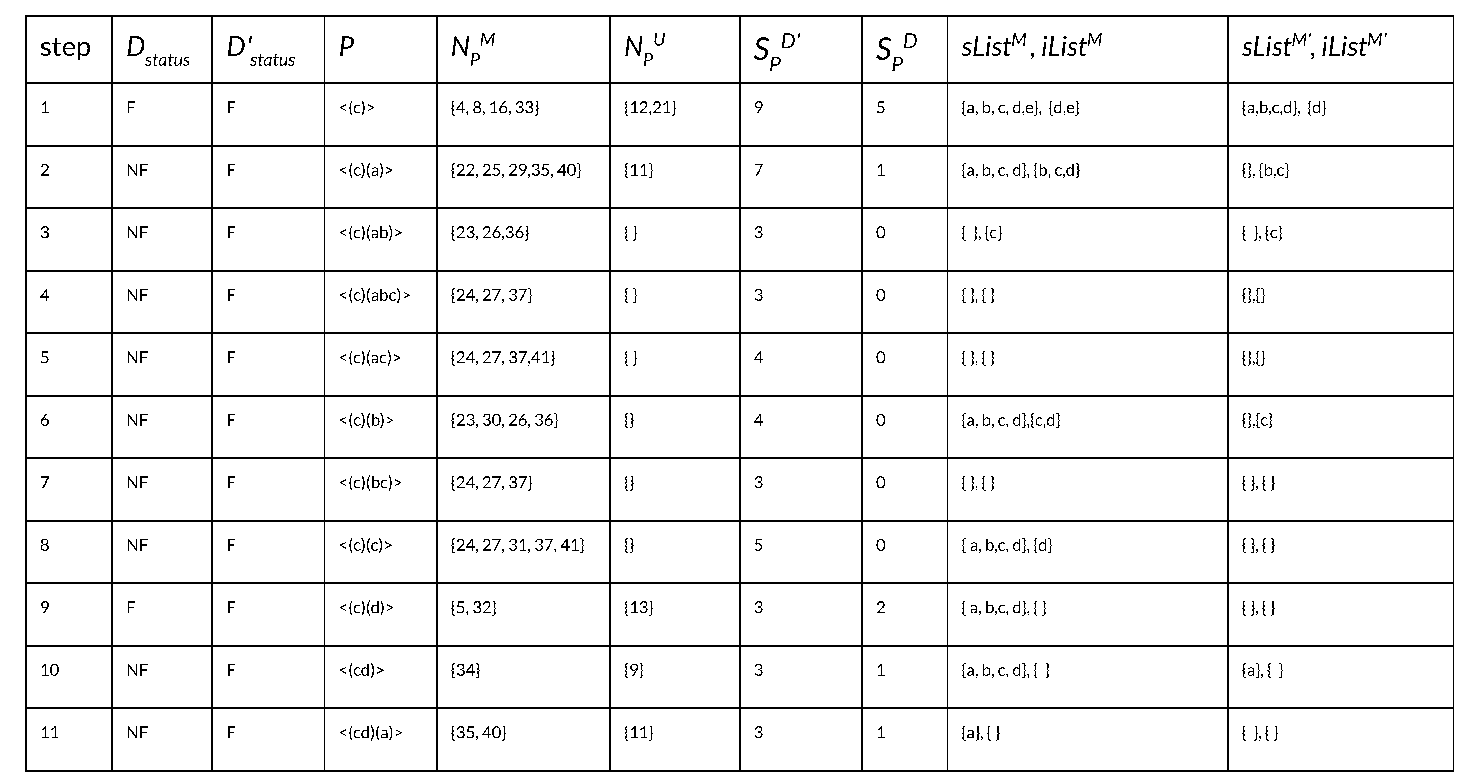
\includegraphics[width=\textwidth]{IncTree-Miner_Simulations}
\caption{Simulation of IncTree-Miner for the patterns with prefix $< (c) >$} \label{figure:inc_tree_miner_simulation}
\hfil
\end{figure*}

\begin{table*}[!htb]
%% increase table row spacing, adjust to taste
%\renewcommand{\arraystretch}{1.3}
% if using array.sty, it might be a good idea to tweak the value of
% \extrarowheight as needed to properly center the text within the cells
\centering
%% Some packages, such as MDW tools, offer better commands for making tables
%% than the plain LaTeX2e tabular which is used here.
\begin{tabular}{|c|c|c|c|c|c|c|c|}
\hline
$P$ & $N_{P}^{M}$ & $T_{P}^{M}$ &$N_{P}^{U}$ & $T_{P}^{U}$ & $S_{P}^{db}$ & $N_{P}^{D^{\prime}}$ & $S_{P}^{D^{\prime}}$\\
\hline
$< (ab) >$ & $\{  23,7,26,36 \}$ & 6 & $\{ 20 \}$ & 1 & 4 & $\{ 23,7,26,36, 20\}$ & 7 \\ \hline
$< (ce) >$ & $\{  28 \}$ & 1 & $\{ 10 \}$ & 1 & 2 & $\{28, 10\}$ & 2\\
\hline
\end{tabular}
\caption{Example of Projection in modified and unmodified subtrees}
\label{table:separate_projection_example}
\end{table*}

\textit{IncTree-Miner} algorithm finds the complete set of frequent patterns from the updated database. After each iteration, basically three types of events can occur - some infrequent patterns become frequent (patterns with completely new prefix or new suffix with the existing ones), some frequent patterns become infrequent and some frequent patterns' support get incremented. Main goal of the IncTree-Miner is to handle these operations efficiently. There are some important observations to highlight in IncTree-Miner,
\begin{definition}[Incremental Support]
    Suppose, we have a pattern $P$ ending at nodes $N_{P}=\{n_{1},n_{2},n_{3},n_{4},n_{5}\}$ where $N_{P}^{U}=\{n_{1},n_{3},n_{5}\}$ are unmodified and $N_{P}^{M}=\{n_{2},n_{4}\}$ are modified nodes. Modified nodes mean those nodes which were affected due to the addition of the IncDB. So, $S_{P}^{D^{\prime}}=C(n_{1})+C(n_{2})+C(n_{3})+C(n_{4})+C(n_{5})$ denotes the total updated support of the pattern  in  $D^{\prime}$ and $S_{P}^{db}=C^{\prime\prime}(n_{2})+C^{\prime\prime}(n_{4})$ denotes the additional support of the pattern occurred due to IncDB ($db$) where $C^{\prime\prime}$=$C-C^{\prime}$ for each modified node.
\end{definition}
\begin{definition}[Infrequent to Frequent Transition Property]
     Suppose, we had an infrequent pattern $P$ (up to previous pass), minimum support threshold value $min\_sup$, previous database $D$ and updated database $D^{\prime}$. The previous minimum support of a pattern to be frequent was $\delta=\ceil{ min\_sup \times \vert D \vert}$ and current is $\delta^{\prime}=\ceil{ min\_sup \times \vert D^{\prime} \vert}$. So, the additional support of $P$ ($S_{P}^{db}$) from the modified subtrees or IncDB needs to be $\geq(\delta^{\prime}-\delta+1)$ for $P$ to be frequent. For the first pass ($\delta=0$), the constraint is $S_{P}^{db}\geq(\delta^{\prime})$ as $D $ is empty.
\end{definition}
IncTree-Miner's basic mining procedure is similar to Tree-Miner except the key point is, it separates the projection nodes of a pattern into two groups, modified nodes and unmodified nodes. It calculates the result separately and merges them and that helps track the changed patterns efficiently. In Fig. \ref{figure:inc_tree_miner_additional_image} (a), we have shown the idea of our pattern mining approach regarding the extensions in modified and unmodified subtrees along with the used terminologies and mathematical relations. Similar to Tree-Miner, our extension functions work based on the proposed breadth-first technique and the complete projection nodes for the patterns are stored in BPFSP-Tree($B$). In Table \ref{table:separate_projection_example}, we have shown two examples of how, IncTree-Miner performs projection in modified and unmodified subtrees separately and then merges them to calculate the complete results for each pattern. To refer the nodes, the IncSP-Tree shown in Fig. \ref{figure:complete_inc_sp_Tree_with_with_two_pass} has been used.

We represent the pattern formation technique in Algorithm \ref{algorithm:pattern_formation_inctree_miner} and the incremental mining technique in Algorithm \ref{algorithm:inc_tree_miner}. A pattern $P\gamma$ can be in three states. It Was previously frequent(Algorithm \ref{algorithm:pattern_formation_inctree_miner}, line 3-10) or its previous complete support is in NIB(lines 11-20) or it  was previously infrequent(lines 21-32). We simulate each case separately. We always first project in modified subtrees(line 2) and based on the results we take decision to perform projection in unmodifed subtrees. We start with the items which were found in IncDB to make the initial $sList^{M}$ and $iList^{M}$(Algorithm \ref{algorithm:inc_tree_miner}), gradually shrink them and track the patterns which were effected or had modifications in underlying subtree. We clear the NIB for the items for which no projection was done in current iteration to maintain consistency. Finally, we remove the unmodified previously frequent but currently infrequent patterns from BPFSP-Tree in a bottom-up manner(Algorithm \ref{algorithm:inc_tree_miner}, lines 27-28). In Fig. \ref{figure:inc_tree_miner_simulation}, a small visualization of IncTree-Miner has been shown where it can be seen, how IncTree-Miner recursively discovers the patterns with prefix $< (c) >$. For each pattern, first its status in old and new database, then its corresponding modified and unmodified projection nodes, its total support calculated from modified and unmodified subtrees, its corresponding two lists and shrinked lists are shown. In Fig. \ref{figure:inc_tree_miner_additional_image} (e), the status of the BPFSP-Tree for the patterns with prefix $< (c) >$ in the old and new database is shown which also reflects how pattern distribution can significantly vary due to database modification. To refer the nodes, the IncSP-Tree shown in Fig. \ref{figure:complete_inc_sp_Tree_with_with_two_pass} has been used.

%  In Fig. \ref{figure:inc_tree_miner_flowchart}, a flowchart has been shown to visualize how IncTree-Miner looks for the extension of a pattern.


IncSP-Tree provides structural advantage to perform faster pattern search in the database. So, it can also help to improve mining performance in buffer based solutions by performing faster pattern generation. Moreover We can also develop a memory resilient IncTree-Miner by not keeping the projection information and performing runtime necessary pattern search using IncSP-Tree. A short visualization of memory resilient version is shown in Fig. \ref{figure:inc_tree_miner_additional_image} (d). In the figure, we have shown that, when we need to know the frequency status of $< (\alpha)(\beta)(\gamma) >$ we perform the projection of it on fly using our tree structure's link properties which help us to perform faster traversals alongside other strategies. Our general proposal focuses on keeping only the frequent pattern's information (pattern and support) to avoid the problem of concept drift. But we can also embed some over computing buffer based approaches here.



%%%%% Logical block representation
%\begin{figure*}[!t]
%\centering
%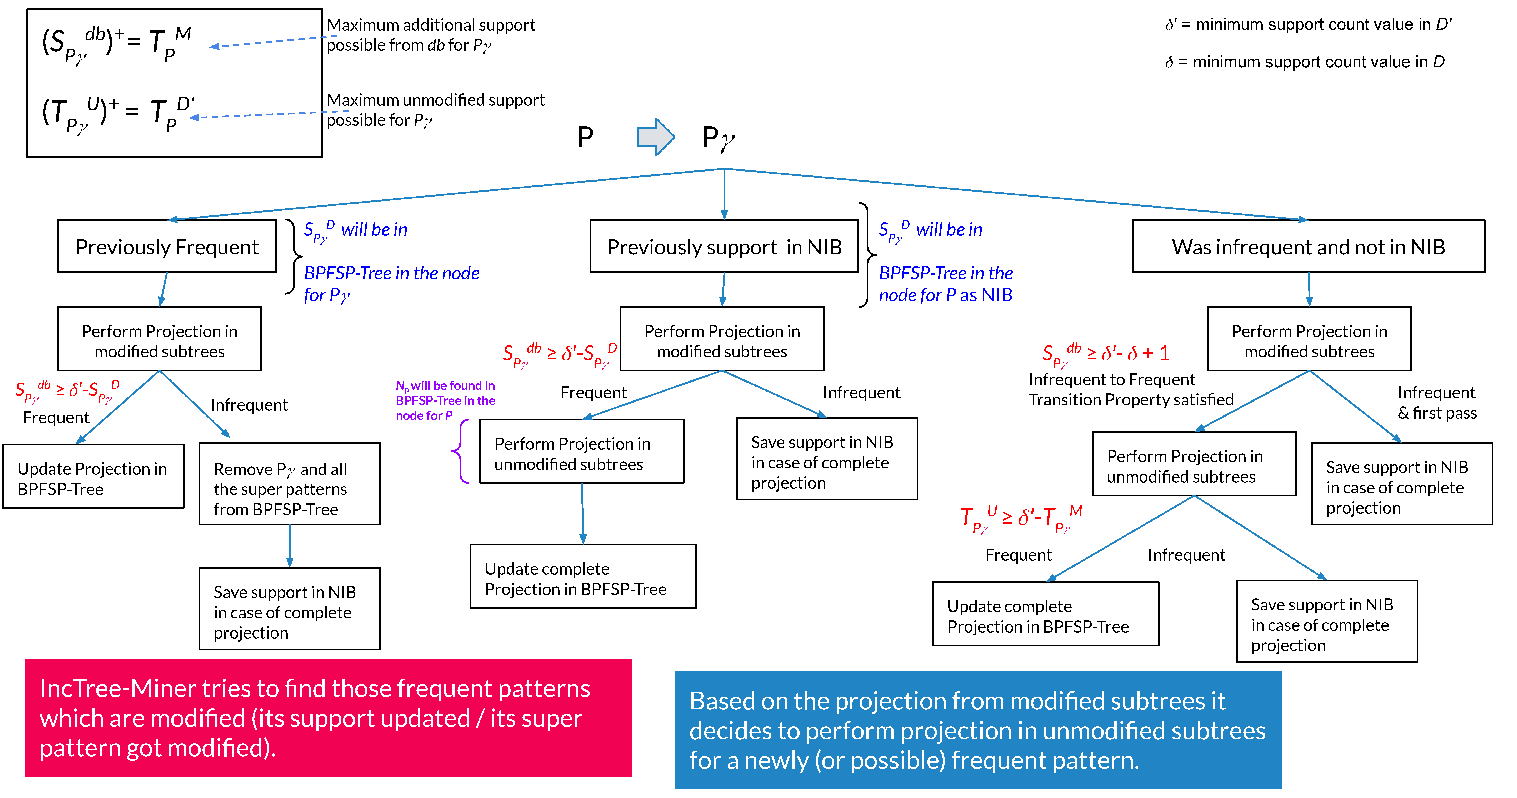
\includegraphics[width=\textwidth]{Inc_Tree_Miner_logical_Block}
%\caption{Logical block representation for pattern extension ($P \,\to\, P\gamma$) in IncTree-Miner}
%\label{figure:inc_tree_miner_flowchart}
%\hfil
%\end{figure*}

\section{Performance Evaluation} \label{evaluation}
In this article, we have proposed two novel tree-based solutions for static and incremental mining problems, namely Tree-Miner based on SP-Tree and IncTree-Miner based on IncSP-Tree. So, during comparison, we considered those popular and state-of-the-art algorithms which were designed as a new mining technique to solve this problem. We also designed a new support counting strategy which helps detect patterns' infrequency early along with some additional pruning strategies.

To compare Tree-Miner, we have considered three popular state-of-the-art mining algorithms, PrefixSpan\cite{han2001prefixspan}, CM-SPAM and CM-SPADE\cite{fournier2014fast} and to compare IncTree-Miner we considered IncSP\cite{lin2004incremental} and PBIncSpan \cite{chen2007incremental}. We have chosen IncSP and PBIncSpan because they are two of the most prominent mining techniques to solve ISPM problem. As these are based on a single minimum support threshold parameter and has similar key factors, there is a solid ground to compare with. We have introduced a new mining approach, so we considered those which did the same. All the implementations were in Python language and the experiments were conducted on a 64-bit machine having Intel Core i5-8265U CPU @ 3.90GHz $\times$ 8, 32 GB RAM, Windows 10 OS.


\subsection{Dataset Description and Parameters}



We have experimented our proposed solutions over various real-life and synthetic datasets. The performance was consistent and matched our intuition.  To discuss the performance we will use the results of the datasets shown in the Table \ref{table:dataset_information_summary}. We have shown the necessary and important information for each dataset in Table \ref{table:dataset_information_summary}. All the real-life datasets are collected from SPMF: A Java Open Source Data Mining Library\footnote{\url{https://www.philippe-fournier-viger.com/spmf/index.php?link=datasets.php}} and synthetic datasets are generated using \textit{IBM Generator} by applying different parameters. In the real-life datasets, all the events had only one single item, so we randomly merged consecutive events to construct multiple itemed events. In Table \ref{table:dataset_information_summary}, we have also shown the average number of itemsets in each sequence ($C$) and average number of items per itemset ($T$) for each dataset after the described modification.

To evaluate our incremental solution, we had to create an incremental mining scenario. To construct the incremental database and represent the common phenomena, we followed the approach mentioned in the relevant literature \cite{lin2004incremental}. Initially, We had the raw database $D_{raw}$, we divided it into two databases, old database $D$ and incremental database $db$. Final updated database was $D^{\prime}$. We have given description of the used variables in Table \ref{table:variables_description}. To understand how the variables work here, we can construct an example using Table \ref{table:static_database} and \ref{table:incremental_database}. Here Table \ref{table:static_database} will work as $D_{raw}$, first iteration of Table \ref{table:incremental_database} will work as $D$ and second iteration of Table \ref{table:incremental_database} will work as $db$. $D_{Append}$ contains 2 sequences or sids ($sid=1$ and $sid=4$) and $D_{Insert}$ contains 4 sequences ($sid=7,8,9,10$). So here $R_{new}=\frac{4\times100}{10}\%=40\%$, $R_{com}=\frac{2 \times 100}{10}\%=20\%$ and $R_{prev}=\frac{(\frac{5}{8}+\frac{2}{5})\times 100\%}{2}=51.25\%$. Here $\frac{5}{8}$ comes from sequence 1 ($sid=1$) which means in the total length of 8 items 5 items appeared in the first pass and the remaining 3 items in the second pass. Same concept applies for $\frac{2}{5}$ for the sequence 4. For conducting experiments, for each dataset, we chose $R_{new}=10\%, R_{com}=50\%$ and $R_{prev}=80\%$ similar to \cite{lin2004incremental}.



We have defined density ratio of a dataset as $d^{*} = \frac{\text{avg. sequence length} \times 100}{\text{(\#)unique items}}$ which is the combination of average sequence length and number of unique items. To evaluate our proposals we have used datasets of both types, highly densed (with high ratio of $d^{*}$) and comparatively much lesser densed.



\begin{table*}[!htb]
%% increase table row spacing, adjust to taste
%\renewcommand{\arraystretch}{1.3}
% if using array.sty, it might be a good idea to tweak the value of
% \extrarowheight as needed to properly center the text within the cells
\centering
%% Some packages, such as MDW tools, offer better commands for making tables
%% than the plain LaTeX2e tabular which is used here.
\begin{tabular}{|c|c|c|c|c|c|c|c|}
\hline
Name & Description & Sequence & Unique & Avg. sequ- & \textit{C} & \textit{T} & $d^{*}$\\
& & Count & Items & ence Length & & &\\
\hline
Bible & Conversion of Bible & 36,369 & 13,905 & 21.64  &  10.97 & 15.49 & 0.16 \\
\hline
MSNBC & Click Stream & 31790 & 17 & 13.23 & 7.83 & 10.81 & 77.82\\
\hline
BMSWebView1 & Click Stream & 59601 & 497 & 2.43 & 2.19 & 6.2 & 0.49\\
\hline
Sign & Sign Language & 730 & 267  & 51.997 & 25.99 & 28.49 & 19.47\\
\hline
Kosarak & Click Stream & 990000 & 41270 & 8.1 & 3.7 & 6.23 & 0.02\\
\hline
L20k-C10-T5-N1K & Synthetic Dataset & 20000 & 1000 & 44.21 &  10 & 5 & 4.42\\
\hline
L50k-C10-T2.5-N10K  & Synthetic Dataset &  50000 & 10000  & 21.79 & 10 & 2.5 & 0.22\\
\hline
\end{tabular}
\caption{Dataset Summarized Information}
\label{table:dataset_information_summary}
\end{table*}


\begin{table*}[!t]
\centering
%% increase table row spacing, adjust to taste
%\renewcommand{\arraystretch}{1.3}
% if using array.sty, it might be a good idea to tweak the value of
% \extrarowheight as needed to properly center the text within the cells
%\centering
%% Some packages, such as MDW tools, offer better commands for making tables
%% than the plain LaTeX2e tabular which is used here.
\begin{tabular}{|l|l|}
\hline
Variable & Description\\ \hline
$D$ & Old database \\ \hline
$db$ & Incremental database, $db=D_{Insert} \cup D_{Append}$. \\ \hline
$D^{\prime}$ & Updated database, $D^{\prime}=D \cup db$.\\ \hline
$R_{new}$ & \textit{New sequence Ratio: }Percentage of sequences completely removed from $D_{raw}$ to put in $D_{Insert}$.\\
&   $|D_{Insert}|=R_{new} \times |D_{raw}|$\\
\hline
$R_{com}$ & \textit{Common Sequence Ratio: }Percentage of common sids picked from $D_{raw}$ to put into $D$ and $D_{Append}$.  \\
& $|D_{Append}| = R_{com} \times |D_{raw}|$.\\
\hline
$R_{prev}$ & \textit{Previous Appearing Ratio: }Avg. splitting ratio for the common sequences lying in  $D$ and $D_{Append}$. \\
& If $R_{prev}=80\%$, then for each common sequence (in avg.) $80\%$ items will be in $D$ and $20\%$ will be \\
& in $D_{Append}$. \\
\hline
$L$ & Total Number of sequences\\ \hline
$C$ & Avg. number of itemsets per sequence \\ \hline
$T$ & Avg. Number of items in each itemset \\ \hline
$N$ & Number of distinct Items \\ \hline
\end{tabular}
\caption{Variables' Description}
\label{table:variables_description}
\end{table*}




\subsection{Tree-Miner}
In this section, we will evaluate Tree-Miner based on various metrics and analyze the results.

\subsubsection{Runtime, Memory Usage and Scalability}
In Fig. \ref{graph:runtime_scalability_comparison_tree_miner} (a)-(g) we present the runtime performance of Tree-Miner. From the corresponding figures, it is obvious that our proposed Tree-Miner based on SP-Tree performs comparatively better than other static mining algorithms. SP-Tree is a compact representation of the database which provides huge structural control over it. Through the next links, we perform efficient traversals in the database which ultimately helps to generate the patterns faster. We also use a set of pruning techniques that significantly reduce the search space. We adopted all the previous pruning techniques and also incorporated some newer ones which makes it a very efficient mining algorithm. In the figures, in lower thresholds, our performance improvement is quite visible because we need to encounter a huge number of patterns and Tree-Miner efficiently discovers them whereas in upper thresholds the performance is quite close because the number of patterns is very small. The performance gets improved in dense datasets through node overlapping characteristics and in sparse datasets through faster database reduction and projection though next links. Our SP-Tree structure is enough to calculate the complete support of the patterns having no necessity to maintain additional structure for each pattern which is also an important factor to improve performance. In Fig. \ref{graph:runtime_scalability_comparison_tree_miner} (a)-(g) we have shown the results for Sign, Bible, BmsWebView1, MSNBC, Kosarak, L20k-C10-T5-N1K and L50k-C10-T2.5-N10K datasets respectively.


\begin{figure*}[!tb]
         \centering
        \begin{subfigure}{.3\linewidth}
         \centering
        \begin{adjustbox}{max width=\textwidth}
         %sign dataset
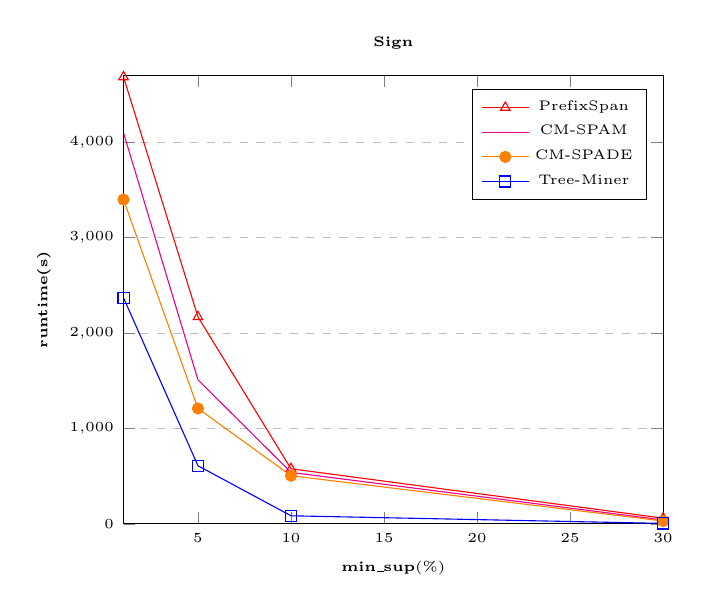
\begin{tikzpicture}
\begin{axis}[
    title={\textbf{Sign}},
    xlabel={$\textbf{min\_sup}$(\%)},
    ylabel={\textbf{runtime(s)}},
    xmin=1, xmax=30,
    ymin=0, ymax=4700,
    %xtick={41, 43, 45, 47, 49, 51, 53, 55},
    %ytick={20, 30, 40, 50, 60, 70, 80, 90, 100, 110, 120, 130, 140},
    legend pos=north east,
    ymajorgrids=true,
    grid style=dashed,
    legend style={font=\tiny},
    title style={font=\tiny},
    label style={font=\tiny},
    every tick label/.append style={font=\tiny}
]
%(41, 12)
%(47, 9)
%(55, 7)
%tree-miner
  \addplot[
    color=red,
    mark=triangle,
    ]
    coordinates {
        (30, 60)
        (10, 578)
        (5, 2170)
        (1, 4685)
    };
    \addlegendentry{PrefixSpan}

    \addplot[
    color=magenta,
    ]
    coordinates {
        (30, 41)
        (10, 540)
        (5, 1510)
        (1, 4100)
    };
    \addlegendentry{CM-SPAM}

    \addplot[
    color=orange,
    mark=*,
    ]
    coordinates {
        (30, 30)
        (10, 505)
        (5, 1210)
        (1, 3400)
    };
    \addlegendentry{CM-SPADE}

    \addplot[
    color=blue,
    mark=square,
    ]
    coordinates {
        (30, 5)
        (10, 85)
        (5, 610)
        (1, 2370)
    };
    \addlegendentry{Tree-Miner}
\end{axis}
\end{tikzpicture}
        \end{adjustbox}
        \caption{}
        \end{subfigure}
        \begin{subfigure}{.3\linewidth}
          \centering
        \begin{adjustbox}{max width=\textwidth}
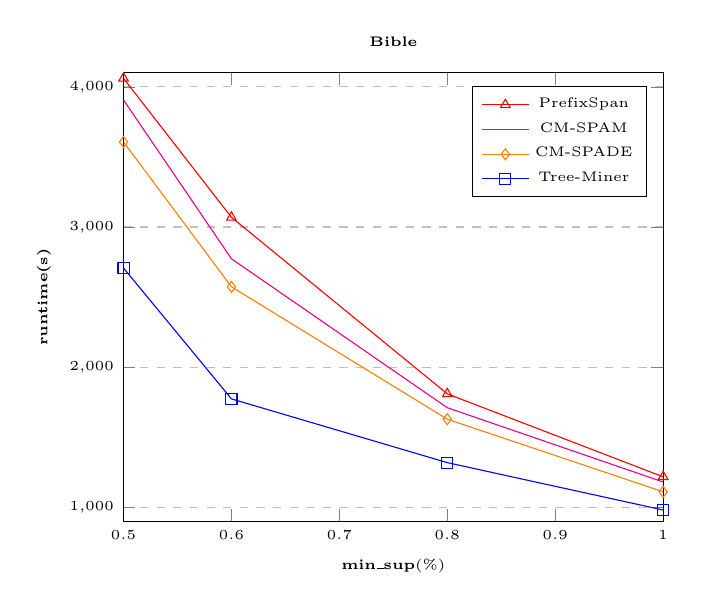
\begin{tikzpicture}
\begin{axis}[
    title={\textbf{Bible}},
   xlabel={$\textbf{min\_sup}$(\%)},
    ylabel={\textbf{runtime(s)}},
    xmin=0.5, xmax=1,
    ymin=900, ymax=4100,
    %xtick={500, 600, 700, 800, 900, 1000},
    %ytick={250, 350, 450, 550, 650, 750, 850, 950, 1050, 1150, 1250, 1350, 1450},
    legend pos=north east,
    ymajorgrids=true,
    grid style=dashed,
    legend style={font=\tiny},
    title style={font=\tiny},
    label style={font=\tiny},
    every tick label/.append style={font=\tiny}
]

%prefixspan
\addplot[
    color=red,
    mark=triangle,
    ]
    coordinates {
        (0.5, 4061)
        (0.6, 3069)
        (0.8, 1809)
        (1, 1217)
    };
    \addlegendentry{PrefixSpan}

  \addplot[
    color=magenta
    ]
    coordinates {
        (0.5, 3907)
        (0.6, 2773)
        (0.8, 1710)
        (1,   1180)
    };
    \addlegendentry{CM-SPAM}

    \addplot[
    color=orange,
    mark=diamond,
    ]
    coordinates {
        (0.5, 3607)
        (0.6, 2573)
        (0.8, 1628)
        (1,   1110)
    };
    \addlegendentry{CM-SPADE}

    %tree-miner
    \addplot[
        color=blue,
        mark=square,
        ]
        coordinates {
            (0.5, 2707)
            (0.6, 1773)
            (0.8, 1318)
            (1,   980)
        };
        \addlegendentry{Tree-Miner}
\end{axis}
\end{tikzpicture}
        \end{adjustbox}
        \caption{}
        \end{subfigure}
        \begin{subfigure}{.3\linewidth}
          \centering
        \begin{adjustbox}{max width=\textwidth}
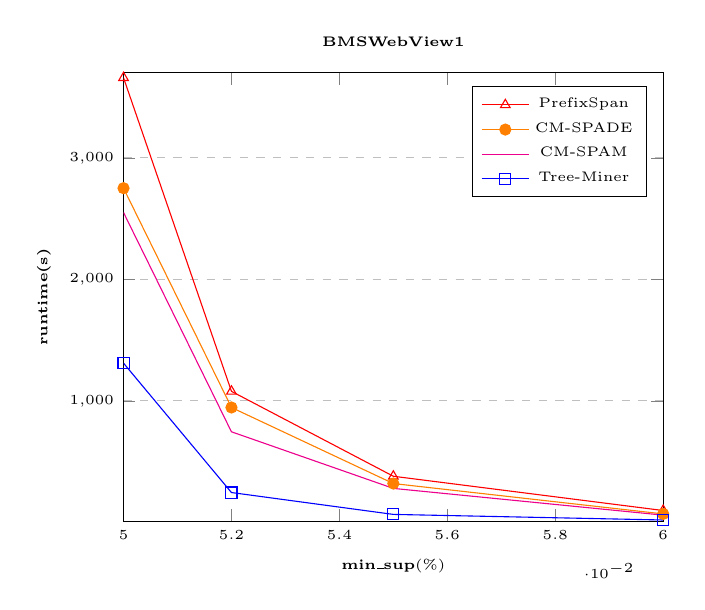
\begin{tikzpicture}
\begin{axis}[
    title={\textbf{BMSWebView1}},
    xlabel={$\textbf{min\_sup}$(\%)},
    ylabel={\textbf{runtime(s)}},
    xmin=0.05, xmax=0.06,
    ymin=10, ymax=3700,
    %xtick={38, 40, 42, 44, 46, 48},
    %ytick={10, 20, 30, 40, 50},
    legend pos=north east,
    ymajorgrids=true,
    grid style=dashed,
    legend style={font=\tiny},
    title style={font=\tiny},
    label style={font=\tiny},
    every tick label/.append style={font=\tiny}
]

\addplot[
    color=red,
    mark=triangle,
    ]
    coordinates {
      (0.06,  98)
      (0.055, 380)
      (0.052, 1079)
      (0.05,  3660)
    };
    \addlegendentry{PrefixSpan}

    \addplot[
    color=orange,
    mark=*
    ]
    coordinates {
        (0.06,  70)
        (0.055, 320)
        (0.052, 946)
        (0.05,  2751)
    };
    \addlegendentry{CM-SPADE}

\addplot[
    color=magenta
    ]
    coordinates {
        (0.06,  60)
        (0.055, 280)
        (0.052, 746)
        (0.05,  2551)
    };
    \addlegendentry{CM-SPAM}


    \addplot[
    color=blue,
    mark=square,
    ]
    coordinates {
        (0.06,  20)
        (0.055, 66)
        (0.052, 246)
        (0.05,  1311)
    };
    \addlegendentry{Tree-Miner}
\end{axis}
\end{tikzpicture}
        \end{adjustbox}
        \caption{}
        \end{subfigure}
        \begin{subfigure}{.3\linewidth}
          \centering
        \begin{adjustbox}{max width=\textwidth}
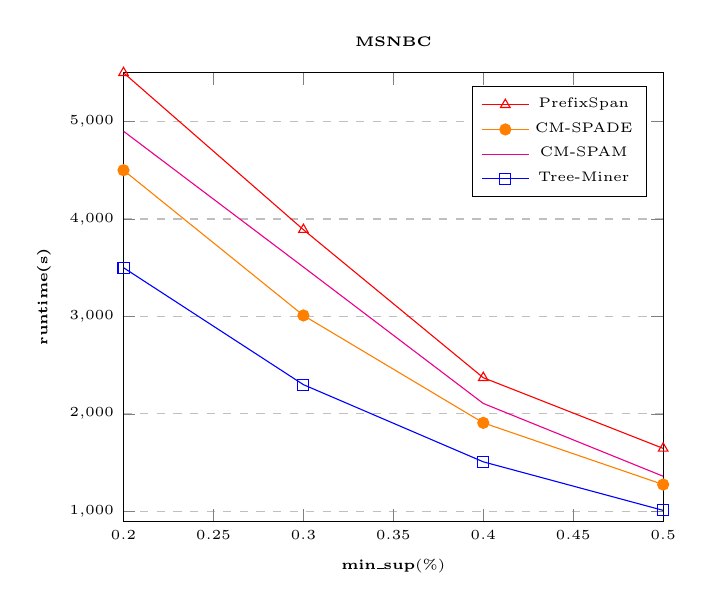
\begin{tikzpicture}
\begin{axis}[
    title={\textbf{MSNBC}},
    xlabel={$\textbf{min\_sup}$(\%)},
    ylabel={\textbf{runtime(s)}},
    xmin=0.2, xmax=0.5,
    ymin=900, ymax=5500,
    %xtick={38, 40, 42, 44, 46, 48},
    %ytick={10, 20, 30, 40, 50},
    legend pos=north east,
    ymajorgrids=true,
    grid style=dashed,
    legend style={font=\tiny},
    title style={font=\tiny},
    label style={font=\tiny},
    every tick label/.append style={font=\tiny}
]

\addplot[
    color=red,
    mark=triangle,
    ]
    coordinates {
        (0.5, 1646)
        (0.4, 2371)
        (0.3, 3890)
        (0.2, 5500)
    };
    \addlegendentry{PrefixSpan}

    \addplot[
    color=orange,
    mark=*
    ]
    coordinates {
        (0.5,  1275)
        (0.4, 1908)
        (0.3, 3010)
        (0.2, 4500)
    };
    \addlegendentry{CM-SPADE}

\addplot[
    color=magenta
    ]
    coordinates {
        (0.5,  1360)
        (0.4, 2107)
        (0.3, 3507)
        (0.2, 4900)
    };
    \addlegendentry{CM-SPAM}


    \addplot[
    color=blue,
    mark=square,
    ]
    coordinates {
        (0.5,  1010)
        (0.4, 1508)
        (0.3, 2300)
        (0.2,  3500)
    };
    \addlegendentry{Tree-Miner}
\end{axis}
\end{tikzpicture}
        \end{adjustbox}
        \caption{}
        \end{subfigure}
        \begin{subfigure}{.3\linewidth}
          \centering
        \begin{adjustbox}{max width=\textwidth}
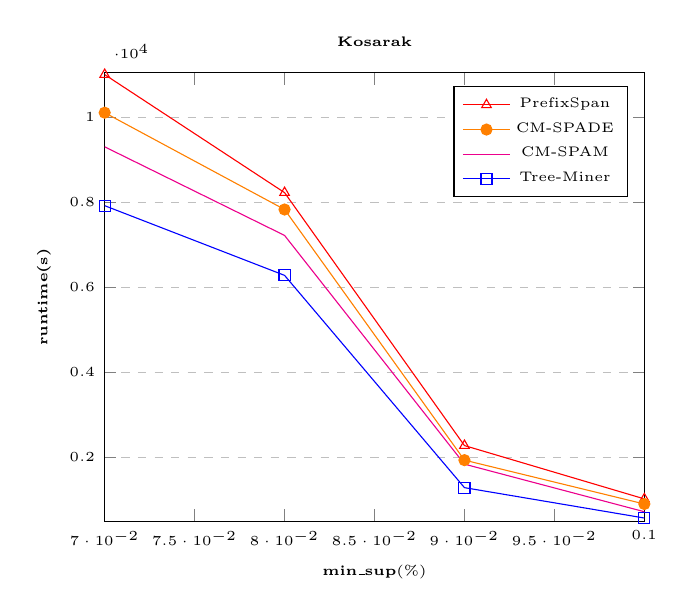
\begin{tikzpicture}
\begin{axis}[
    title={\textbf{Kosarak}},
    xlabel={$\textbf{min\_sup}$(\%)},
    ylabel={\textbf{runtime(s)}},
    xmin=0.07, xmax=0.1,
    ymin=500, ymax=11050,
    %xtick={38, 40, 42, 44, 46, 48},
    %ytick={10, 20, 30, 40, 50},
    legend pos=north east,
    ymajorgrids=true,
    grid style=dashed,
   legend style={font=\tiny},
    title style={font=\tiny},
    label style={font=\tiny},
    every tick label/.append style={font=\tiny}
]

\addplot[
    color=red,
    mark=triangle,
    ]
    coordinates {
        (0.1,   1025)
        (0.09,  2280)
        (0.08,  8232)
        (0.07,  11010)
    };
    \addlegendentry{PrefixSpan}

    \addplot[
    color=orange,
    mark=*
    ]
    coordinates {
        (0.1,905)
        (0.09,1937)
        (0.08,7835)
        (0.07,10113)
    };
    \addlegendentry{CM-SPADE}

  \addplot[
    color=magenta
    ]
    coordinates {
        (0.1,723)
        (0.09,1843)
        (0.08,7225)
        (0.07,9310)
    };
    \addlegendentry{CM-SPAM}


    \addplot[
    color=blue,
    mark=square,
    ]
    coordinates {
        (0.1,575)
        (0.09,1290)
        (0.08,6285)
        (0.07,7925)
    };
    \addlegendentry{Tree-Miner}
\end{axis}
\end{tikzpicture}
        \end{adjustbox}
         \caption{}
        \end{subfigure}
        \begin{subfigure}{.3\linewidth}
          \centering
        \begin{adjustbox}{max width=\textwidth}
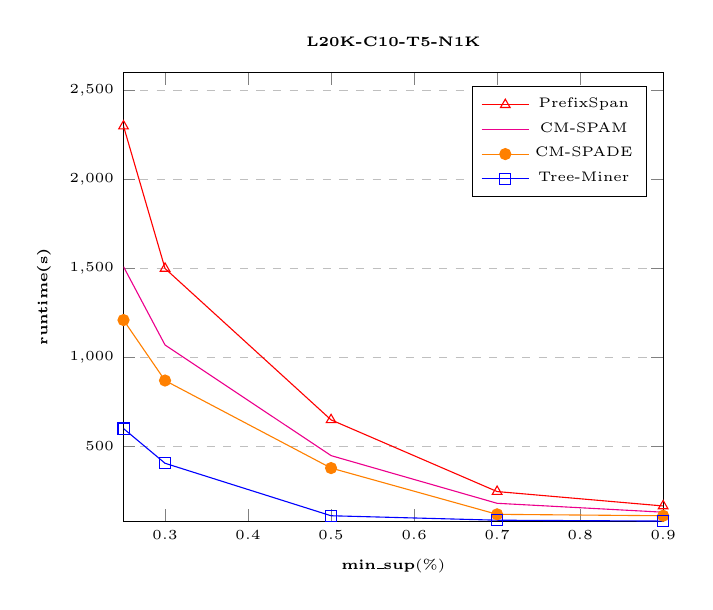
\begin{tikzpicture}
\begin{axis}[
    title={\textbf{L20K-C10-T5-N1K}},
    xlabel={$\textbf{min\_sup}$(\%)},
    ylabel={\textbf{runtime(s)}},
    xmin=0.25, xmax=0.9,
    ymin=80, ymax=2600,
    %xtick={38, 40, 42, 44, 46, 48},
    %ytick={10, 20, 30, 40, 50},
    legend pos=north east,
    ymajorgrids=true,
    grid style=dashed,
    legend style={font=\tiny},
    title style={font=\tiny},
    label style={font=\tiny},
    every tick label/.append style={font=\tiny}
]

\addplot[
    color=red,
    mark=triangle,
    ]
    coordinates {
        (0.9,  165)
        (0.7,  246)
        (0.5, 649)
        (0.3,  1500)
        (0.25, 2300)
    };
    \addlegendentry{PrefixSpan}

    \addplot[
    color=magenta
    ]
    coordinates {
        (0.9,  130)
        (0.7,  180)
        (0.5, 448)
        (0.3,  1070)
        (0.25, 1510)
    };
    \addlegendentry{CM-SPAM}

    \addplot[
    color=orange,
    mark=*
    ]
    coordinates {
        (0.9,  110)
        (0.7,  118)
        (0.5, 378)
        (0.3,  870)
        (0.25, 1210)
    };
    \addlegendentry{CM-SPADE}


    \addplot[
    color=blue,
    mark=square,
    ]
    coordinates {
        (0.9,  80)
        (0.7, 85)
        (0.5, 110)
        (0.3,  405)
        (0.25, 600)
    };
    \addlegendentry{Tree-Miner}
\end{axis}
\end{tikzpicture}
        \end{adjustbox}
         \caption{}
        \end{subfigure}
        \begin{subfigure}{.3\linewidth}
          \centering
        \begin{adjustbox}{max width=\textwidth}
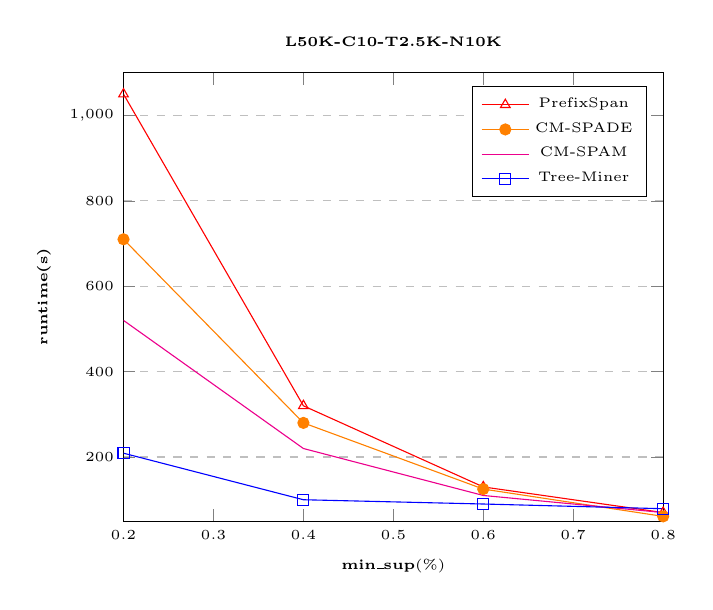
\begin{tikzpicture}
\begin{axis}[
    title={\textbf{L50K-C10-T2.5K-N10K}},
    xlabel={$\textbf{min\_sup}$(\%)},
    ylabel={\textbf{runtime(s)}},
    xmin=0.2, xmax=0.8,
    ymin=50, ymax=1100,
    %xtick={38, 40, 42, 44, 46, 48},
    %ytick={10, 20, 30, 40, 50},
    legend pos=north east,
    ymajorgrids=true,
    grid style=dashed,
   legend style={font=\tiny},
    title style={font=\tiny},
    label style={font=\tiny},
    every tick label/.append style={font=\tiny}
]

\addplot[
    color=red,
    mark=triangle,
    ]
    coordinates {
        (0.8,  70)
        (0.6, 130)
        (0.4, 320)
        (0.2,  1050)
    };
    \addlegendentry{PrefixSpan}

    \addplot[
    color=orange,
    mark=*
    ]
    coordinates {
        (0.8,  61)
        (0.6, 125)
        (0.4, 280)
        (0.2, 710)
    };
    \addlegendentry{CM-SPADE}

  \addplot[
    color=magenta
    ]
    coordinates {
        (0.8,  70)
        (0.6, 110)
        (0.4, 220)
        (0.2, 520)
    };
    \addlegendentry{CM-SPAM}


    \addplot[
    color=blue,
    mark=square,
    ]
    coordinates {
        (0.8,  79)
        (0.6, 90)
        (0.4, 100)
        (0.2,  209)
    };
    \addlegendentry{Tree-Miner}
\end{axis}
\end{tikzpicture}
        \end{adjustbox}
         \caption{}
        \end{subfigure}
        \begin{subfigure}{.3\linewidth}
            \begin{adjustbox}{max width=\textwidth}
            \centering
           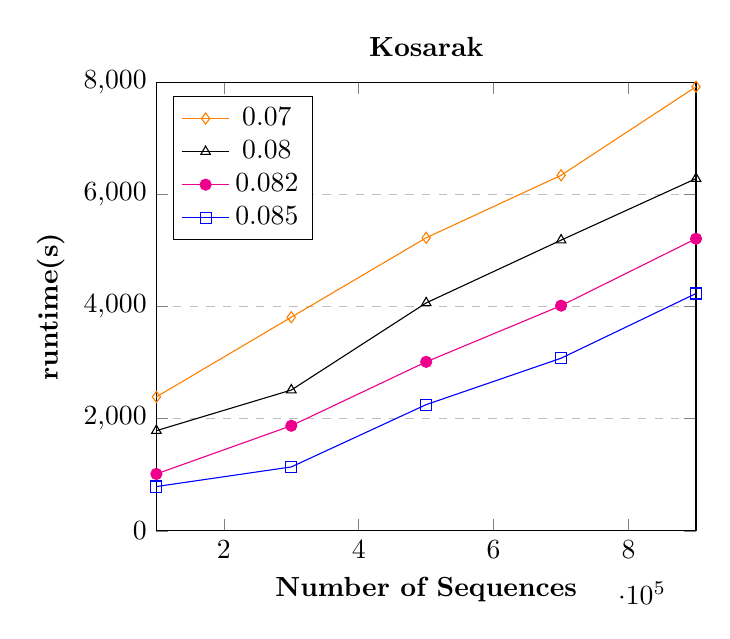
\begin{tikzpicture}
              \begin{axis}[
    title={\textbf{Kosarak}},
    xlabel={\textbf{Number of Sequences}},
    ylabel={\textbf{runtime(s)}},
    xmin=100000, xmax=900000,
    ymin=0, ymax=8000,
    legend pos=north west,
    ymajorgrids=true,
    grid style=dashed,
]
    \addplot[
    color=orange,
    mark=diamond,
    ]
    coordinates {
      (900000,7925)
      (700000,6344)
      (500000,5229)
      (300000,3812)
      (100000,2390)
    };
    \addplot[
    color=black,
    mark=triangle
    ]
    coordinates {
      (900000,6285)
      (700000,5187)
      (500000,4067)
      (300000,2512)
      (100000,1787)
    };
    \addplot[
    color=magenta,
    mark=*,
    ]
    coordinates {
        (900000,5212)
        (700000,4018)
        (500000,3015)
        (300000,1875)
        (100000,1015)
    };
    \addplot[
        color=blue,
        mark=square,
        ]
        coordinates {
         (900000,4235)
         (700000,3080)
         (500000,2252)
         (300000,1140)
         (100000,790)
        };
    \legend{0.07, 0.08, 0.082, 0.085}
\end{axis}
           \end{tikzpicture}
           \end{adjustbox}
           \caption{}
           \end{subfigure}

        \caption{(a) - (g): Runtime Comparisons, (h) Scalability Comparison for Tree-Miner}
        \label{graph:runtime_scalability_comparison_tree_miner}
        \end{figure*}

\textcolor{blue}{up to now, the comparison has been shown with the base mining approaches as the proposed solution was designed as a new mining algorithm for SPM problem. We have also tried to apply the proposed solution in some different types of SPM problems which are mostly application centric and borrows concepts from base pattern mining techniques.}


\textcolor{blue}{In this regard, we compared our proposal with \cite{he2019significance} and \cite{tarus2018hybrid} two recent literatures. In \cite{he2019significance}, they mined discriminative sequential patterns using significance threshold. Here they first generate all the frequent patterns using GSP, then conduct multi level correlation analysis in such regard. In \cite{tarus2018hybrid}, they designed a context based e-learning recommendation system using the utility of SPM algorithms where GSP was used in such regard. We applied our proposal in these literatures and could directly embed it without any modification. As pattern growth approaches are significantly faster compared to GSP, our Tree-Miner improved the performance of the pattern generation level to a significant amount leading to an overall improvement. Some experimental results have been provided to support the claim in Fig \ref{figure:runtime_with_gsp}. For the comparisons, all the base datasets have been used here, multiple single itemed  sequential events.}

\textcolor{blue}{In the figure (a) and (b) shows the results of Tree-Miner embedded performance improvement where Disc denotes the applied solution in literature \cite{he2019significance} whereas Tree-Miner with Disc denotes our solution. For the comparison here, significance level ($\alpha$) as per stated in the article is fixed and the support threshold value is varied.}

\textcolor{blue}{Similarly, some results have been shown after comparing with \cite{tarus2018hybrid}. In this article, a recommendation system is built based on context awareness for e-learning purpose. For this purpose, they needed relevant web click stream data, users' knowledge profile and ratings for each resource upon which they calculated the suggestion metrics. To bring the context aware recommendation, they used GSP to filter out the suggestions after generating a set of frequent sequential patterns or web logs visited by the users. Keeping all their contributions align, the comparison comes here is how the pattern generation process can be made faster using our proposal. In Fig. \ref{figure:runtime_with_gsp} (c) and (d), we have shown the performance of GSP with Tree-Miner in two click stream datasets. Here we have used the base datasets, single event with multiple itemed events for the comparison.}
\begin{figure*}[!tb]
            \centering
        \begin{subfigure}{.24\linewidth}
          \centering
        \begin{adjustbox}{max width=\textwidth}
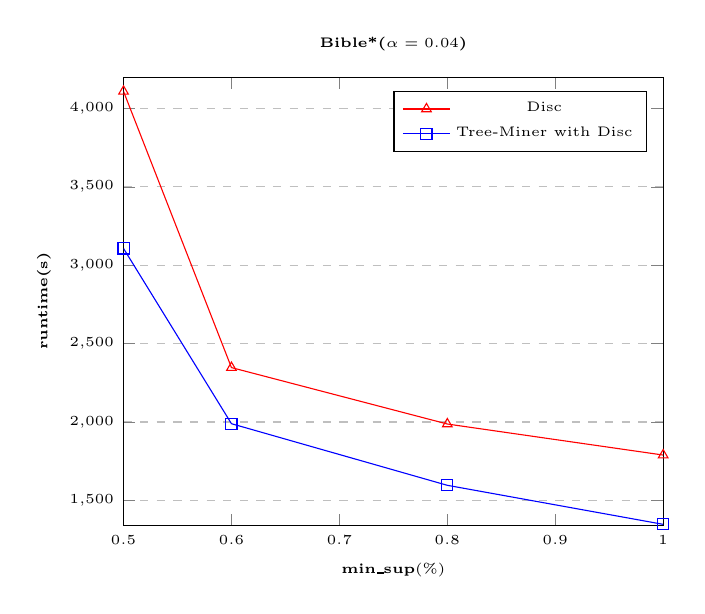
\begin{tikzpicture}
\begin{axis}[
    title={\textbf{Bible*($\alpha=0.04$)}},
    xlabel={$\textbf{min\_sup}$(\%)},
    ylabel={\textbf{runtime(s)}},
    xmin=0.5, xmax=1,
    ymin=1340, ymax=4200,
    %xtick={38, 40, 42, 44, 46, 48},
    %ytick={10, 20, 30, 40, 50},
    legend pos=north east,
    ymajorgrids=true,
    grid style=dashed,
   legend style={font=\tiny},
    title style={font=\tiny},
    label style={font=\tiny},
    every tick label/.append style={font=\tiny}
]

\addplot[
    color=red,
    mark=triangle,
    ]
    coordinates {
        (0.5, 4109)
        (0.6, 2347)
        (0.8, 1987)
        (1,   1789)
    };
    \addlegendentry{Disc}

    \addplot[
    color=blue,
    mark=square,
    ]
    coordinates {
        (0.5, 3107)
        (0.6, 1989)
        (0.8, 1596)
        (1,   1347)
    };
    \addlegendentry{Tree-Miner with Disc}
\end{axis}
\end{tikzpicture}
        \end{adjustbox}
         \caption{}
        \end{subfigure}
        \begin{subfigure}{.24\linewidth}
          \centering
        \begin{adjustbox}{max width=\textwidth}
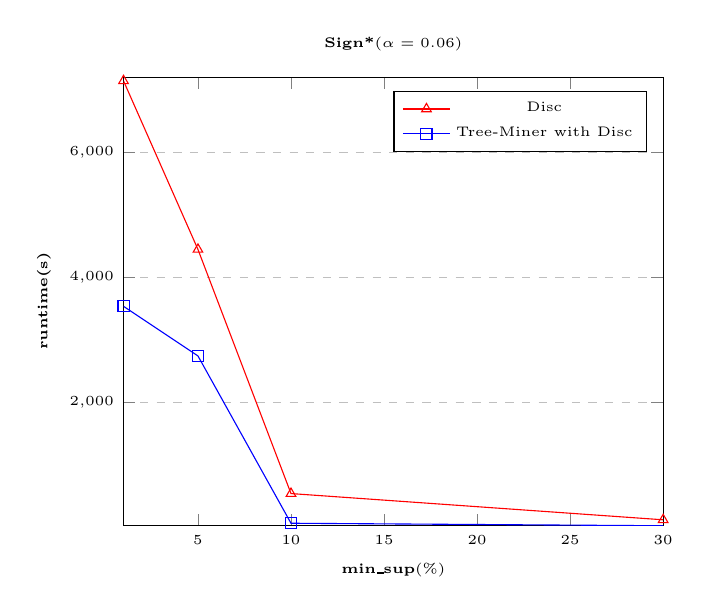
\begin{tikzpicture}
\begin{axis}[
    title={\textbf{Sign*$(\alpha=0.06)$}},
    xlabel={$\textbf{min\_sup}$(\%)},
    ylabel={\textbf{runtime(s)}},
    xmin=1, xmax=30,
    ymin=40, ymax=7200,
    %xtick={38, 40, 42, 44, 46, 48},
    %ytick={10, 20, 30, 40, 50},
    legend pos=north east,
    ymajorgrids=true,
    grid style=dashed,
    legend style={font=\tiny},
    title style={font=\tiny},
    label style={font=\tiny},
    every tick label/.append style={font=\tiny}
]

\addplot[
    color=red,
    mark=triangle,
    ]
    coordinates {
        (30,130)
        (10, 549)
        (5, 4448)
        (1, 7140)
    };
    \addlegendentry{Disc}

    \addplot[
    color=blue,
    mark=square,
    ]
    coordinates {
        (30,35)
        (10, 75)
        (5, 2747)
        (1, 3540)
    };
    \addlegendentry{Tree-Miner with Disc}
\end{axis}
\end{tikzpicture}
        \end{adjustbox}
        \caption{}
        \end{subfigure}
        \begin{subfigure}{.24\linewidth}
          \centering
        \begin{adjustbox}{max width=\textwidth}
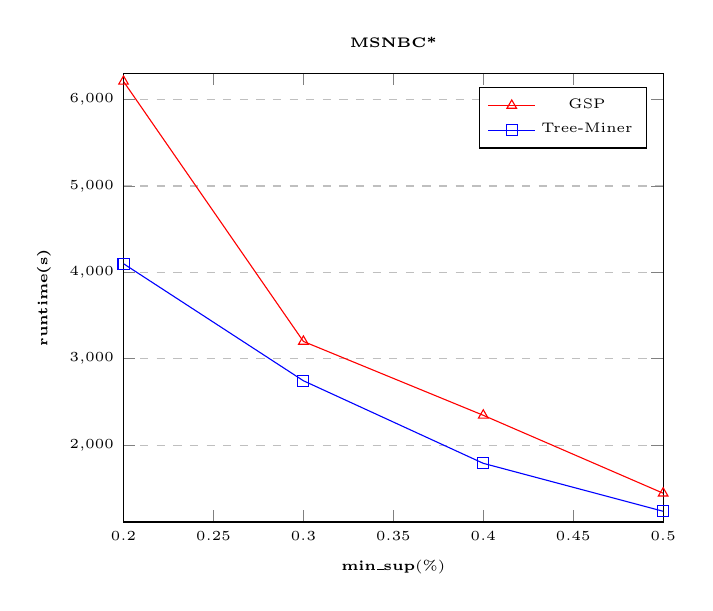
\begin{tikzpicture}
\begin{axis}[
    title={\textbf{MSNBC*}},
    xlabel={$\textbf{min\_sup}$(\%)},
    ylabel={\textbf{runtime(s)}},
    xmin=0.2, xmax=0.5,
    ymin=1110, ymax=6300,
    %xtick={38, 40, 42, 44, 46, 48},
    %ytick={10, 20, 30, 40, 50},
    legend pos=north east,
    ymajorgrids=true,
    grid style=dashed,
    legend style={font=\tiny},
    title style={font=\tiny},
    label style={font=\tiny},
    every tick label/.append style={font=\tiny}
]

\addplot[
    color=red,
    mark=triangle,
    ]
    coordinates {
        (0.5, 1443)
        (0.4, 2345)
        (0.3, 3200)
        (0.2,  6210)
    };
    \addlegendentry{GSP}

    \addplot[
    color=blue,
    mark=square,
    ]
    coordinates {
        (0.5,  1234)
        (0.4, 1789)
        (0.3, 2745)
        (0.2,  4100)
    };
    \addlegendentry{Tree-Miner}
\end{axis}
\end{tikzpicture}
        \end{adjustbox}
        \caption{}
        \end{subfigure}
        \begin{subfigure}{.24\linewidth}
          \centering
        \begin{adjustbox}{max width=\textwidth}
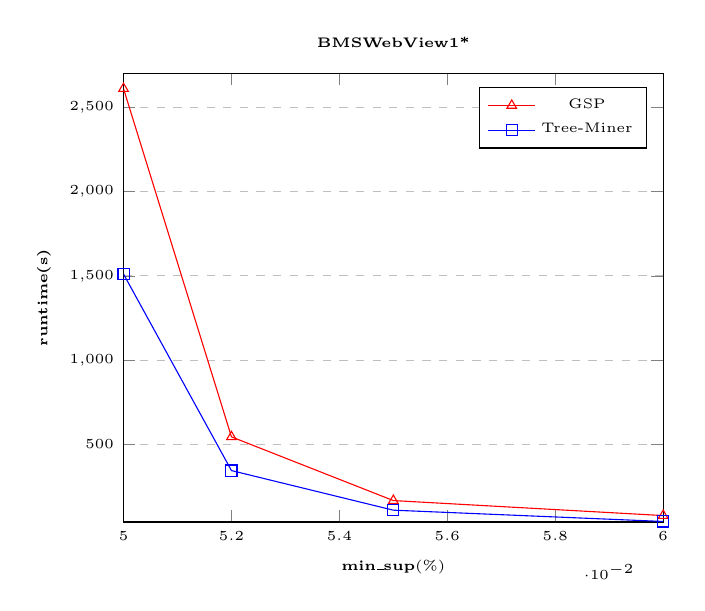
\begin{tikzpicture}
\begin{axis}[
    title={\textbf{BMSWebView1*}},
    xlabel={$\textbf{min\_sup}$(\%)},
    ylabel={\textbf{runtime(s)}},
    xmin=0.05, xmax=0.06,
    ymin=40, ymax=2700,
    %xtick={38, 40, 42, 44, 46, 48},
    %ytick={10, 20, 30, 40, 50},
    legend pos=north east,
    ymajorgrids=true,
    grid style=dashed,
    legend style={font=\tiny},
    title style={font=\tiny},
    label style={font=\tiny},
    every tick label/.append style={font=\tiny}
]

\addplot[
    color=red,
    mark=triangle,
    ]
    coordinates {
        (0.06,  78)
        (0.055, 167)
        (0.052, 545)
        (0.05,  2611)
    };
    \addlegendentry{GSP}

    \addplot[
    color=blue,
    mark=square,
    ]
    coordinates {
        (0.06,  43)
        (0.055, 110)
        (0.052, 345)
        (0.05,  1511)
    };
    \addlegendentry{Tree-Miner}
\end{axis}
\end{tikzpicture}
        \end{adjustbox}
        \caption{}
        \end{subfigure}
        \caption{\textcolor{blue}{Runtime Improvement using Tree-Miner over GSP based literature}}
        \label{figure:runtime_with_gsp}
        \end{figure*}

\textcolor{blue}{We have also compared our solution to \cite{hosseininasab2019constraint}, a novel Mining with Decision Diagram (MDD) based approach to solve constraint-based sequential pattern mining. But to make a fair comparison with the literature's solution, we had to modify our algorithm and datasets to some extent. A summary of such modifications are shown as below,}

\textcolor{blue}{\begin{itemize}
    \item In the literature, how multiple itemed event will be handled was not proposed. So, for the comparisons, all the base datasets have been used here, multiple single itemed  sequential events.
    \item The literature constructed their proposed MDD nodes over an initially given support threshold value by pruning nodes. This idea can easily be embedded in our solution as ours is more generic. When the next links are calculated, we can apply the breadth-first and upper bound based pattern generation concept to reduce many next link connection.\\
    For example, we want to generate $\alpha \,\to\, \alpha\beta$. Here $N_{\alpha}=\{2, 3, 4\}$, $S_{\alpha}=9$, $C(2)=C(3)=C(4)=3$, $\delta=8$. We want to calculate next links for $\beta$ from each $v\in N_{\alpha}$. Let from $2$ we need to make a next link connection with $5$ for $\beta$ where $C(5)=1$. So using breadth-first technique, we can see $S_{\alpha\beta}=9-3+1<\delta$. Thus we can stop constructing all the next links for $\alpha \,\to \, \beta$ and its super patterns for all the remaining nodes along with pruning this pattern from the generation.
    \item Two solutions' comparisons are done only over support threshold constraint. The result is shown in Fig. \ref{graph:runtime_comparison_with_mdd}.
\end{itemize}}

\begin{figure*}[!tb]
            \centering
        \begin{subfigure}{.3\linewidth}
          \centering
        \begin{adjustbox}{max width=\textwidth}
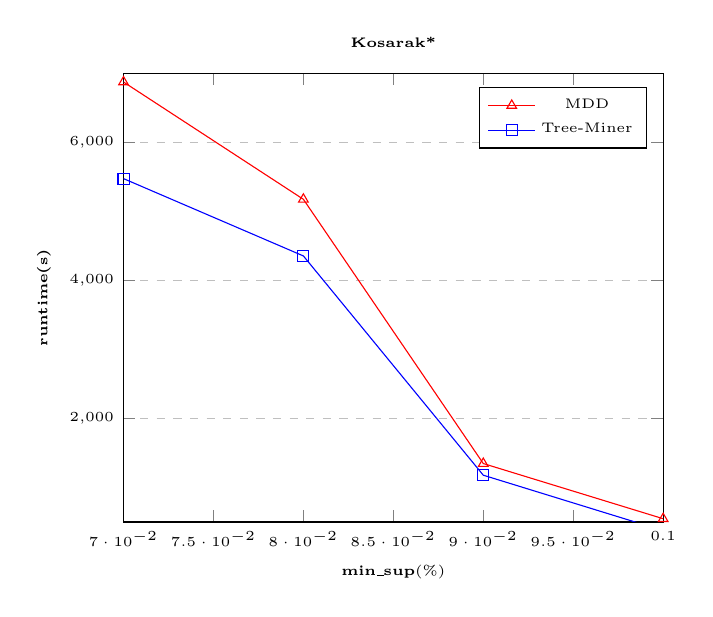
\begin{tikzpicture}
\begin{axis}[
    title={\textbf{Kosarak*}},
    xlabel={$\textbf{min\_sup}$(\%)},
    ylabel={\textbf{runtime(s)}},
    xmin=0.07, xmax=0.1,
    ymin=500, ymax=7000,
    %xtick={38, 40, 42, 44, 46, 48},
    %ytick={10, 20, 30, 40, 50},
    legend pos=north east,
    ymajorgrids=true,
    grid style=dashed,
   legend style={font=\tiny},
    title style={font=\tiny},
    label style={font=\tiny},
    every tick label/.append style={font=\tiny}
]

\addplot[
    color=red,
    mark=triangle,
    ]
    coordinates {
        (0.1,547)
        (0.09,1347)
        (0.08,5178)
        (0.07,6879)
    };
    \addlegendentry{MDD}

    \addplot[
    color=blue,
    mark=square,
    ]
    coordinates {
        (0.1,374)
        (0.09,1178)
        (0.08,4357)
        (0.07,5478)
    };
    \addlegendentry{Tree-Miner}
\end{axis}
\end{tikzpicture}
        \end{adjustbox}
         \caption{}
        \end{subfigure}
        \begin{subfigure}{.3\linewidth}
          \centering
        \begin{adjustbox}{max width=\textwidth}
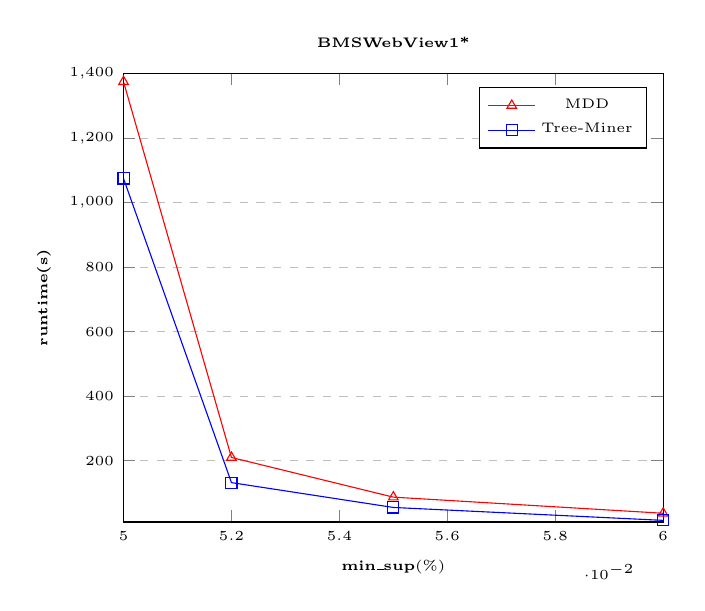
\begin{tikzpicture}
\begin{axis}[
    title={\textbf{BMSWebView1*}},
    xlabel={$\textbf{min\_sup}$(\%)},
    ylabel={\textbf{runtime(s)}},
    xmin=0.05, xmax=0.06,
    ymin=10, ymax=1400,
    %xtick={38, 40, 42, 44, 46, 48},
    %ytick={10, 20, 30, 40, 50},
    legend pos=north east,
    ymajorgrids=true,
    grid style=dashed,
    legend style={font=\tiny},
    title style={font=\tiny},
    label style={font=\tiny},
    every tick label/.append style={font=\tiny}
]

\addplot[
    color=red,
    mark=triangle,
    ]
    coordinates {
      (0.06,  37)
        (0.055, 87)
        (0.052, 210)
        (0.05,  1375)
    };
    \addlegendentry{MDD}

    \addplot[
    color=blue,
    mark=square,
    ]
    coordinates {
        (0.06,  15)
        (0.055, 55)
        (0.052, 132)
        (0.05,  1075)
    };
    \addlegendentry{Tree-Miner}
\end{axis}
\end{tikzpicture}
        \end{adjustbox}
        \caption{}
        \end{subfigure}
        \begin{subfigure}{.3\linewidth}
          \centering
        \begin{adjustbox}{max width=\textwidth}
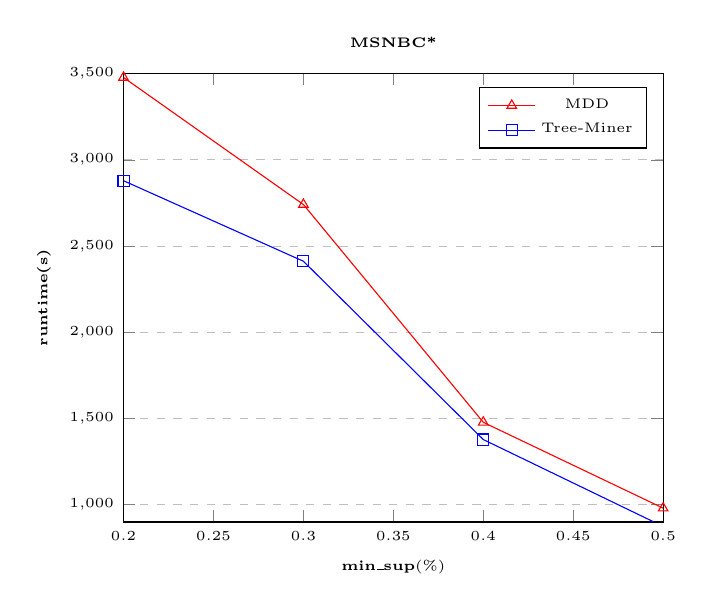
\begin{tikzpicture}
\begin{axis}[
    title={\textbf{MSNBC*}},
    xlabel={$\textbf{min\_sup}$(\%)},
    ylabel={\textbf{runtime(s)}},
    xmin=0.2, xmax=0.5,
    ymin=900, ymax=3500,
    %xtick={38, 40, 42, 44, 46, 48},
    %ytick={10, 20, 30, 40, 50},
    legend pos=north east,
    ymajorgrids=true,
    grid style=dashed,
    legend style={font=\tiny},
    title style={font=\tiny},
    label style={font=\tiny},
    every tick label/.append style={font=\tiny}
]

\addplot[
    color=red,
    mark=triangle,
    ]
    coordinates {
        (0.5, 980)
        (0.4, 1478)
        (0.3, 2741)
        (0.2, 3478)
    };
    \addlegendentry{MDD}

    \addplot[
    color=blue,
    mark=square,
    ]
    coordinates {
        (0.5,  874)
        (0.4, 1378)
        (0.3, 2412)
        (0.2,  2879)
    };
    \addlegendentry{Tree-Miner}
\end{axis}
\end{tikzpicture}
        \end{adjustbox}
        \caption{}
        \end{subfigure}
        \caption{\textcolor{blue}{Runtime Comparisons between Tree-Miner and MDD}}
        \label{graph:runtime_comparison_with_mdd}
        \end{figure*}

\textcolor{blue}{From the figures, it can be observed that Tree-Miner with SP-Tree performs comparatively better. The main reasons lie in its larger flexibility, e.g., multiple event handling, easily modifiable, bit based usage advantages, etc and pruning strategies. The results for Kosarak, MSNBC and BMSWebView1 have been shown in the figure. As previously stated, using next links we can perform faster jumps in the database along with using the rich pruning techniques a good amount of pattern searching can be omitted.}


Due to the structured representation of the information, our solution needs comparatively more memory. We maintain SP-Tree and co-occurrence information which gives control over the database and helps significantly during pattern extension. Prefixspan uses database projection technique, CM-SPADE uses lattice alike structures and CM-SPAM uses bit based array structures to perform projection and calculate the support of a pattern. During pattern extension, the compared algorithms create and maintain some sort of additional supporting structures in runtime whereas our proposed solution uses the base tree structures' nodes for this purpose. Through some additional memory usage, we gain significant amount of improvement in mining which we will show shortly and considering the runtime improvement this should be tolerable. We present an analysis in Fig. \ref{graph:memory_comparison_tree_miner} for two datasets. From the figure, it can be seen that our solution comparatively needs some additional memory and we have already discussed the underlying reasoning behind it. The difference will be comparatively closer in denser datasets due to tree's node overlapping characteristics.

We have also conducted a scalability analysis of Tree-Miner and presented the result in Fig. \ref{graph:runtime_scalability_comparison_tree_miner} (g) experimenting over the lage \textit{Kosarak} dataset. We started with 100000 transactions, gradually increased it and recorded the performance for various $min\_sup$. The corresponding figure shows the linear scalability of the solution. Another important concern can be, as our solution is based on defined structures, do their construction times create any bottleneck during mining. For this purpose we present an analysis in Table \ref{table:construction_time_tree_miner} where we can see that, the total construction time is quite insignificant compared to the total mining time and does not create bottleneck. In the last three columns of Table \ref{table:construction_time_tree_miner} we have also shown the corresponding runtime performance improvement in mining over the comparing algorithms ($Pr$: PrefixSpan, $SP$: CM-SPADE, $SM$: CM-SPAM). This basically states the significance of how much we can improve mining performance with very small time cost in pre-processing.



\begin{figure*}[!tb]
            \centering
        \begin{subfigure}{0.4\linewidth}
\centering
 \begin{adjustbox}{max width=\textwidth}
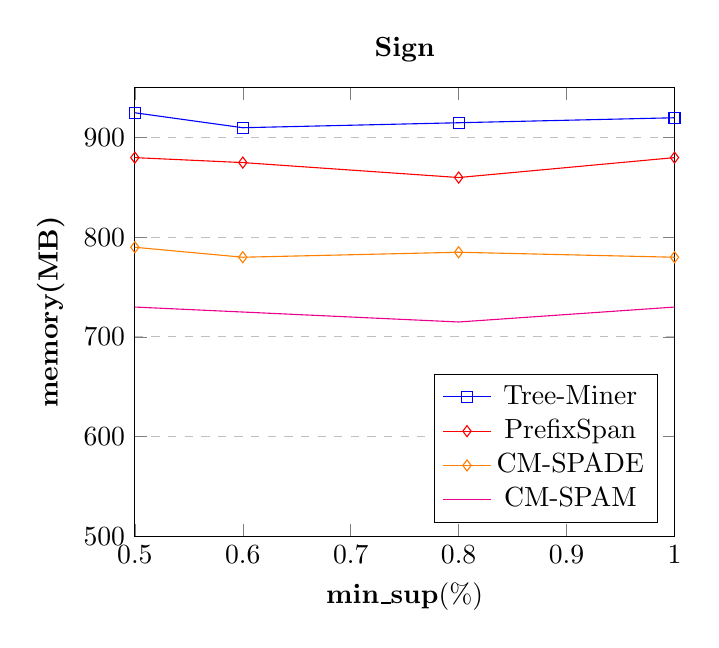
\begin{tikzpicture}
\begin{axis}[
    title={\textbf{Sign}},
    xlabel={$\textbf{min\_sup}$(\%)},
    ylabel={\textbf{memory(MB)}},
    xmin=0.5, xmax=1,
    ymin=500, ymax=950,
    %xtick={1200, 1500, 2000},
    %ytick={0,2,4,6,8},
    legend pos=south east,
    ymajorgrids=true,
    grid style=dashed,
]

%(41, 12)
%(47, 9)
%(55, 7)

%tree-miner
\addplot[
    color=blue,
    mark=square,
    ]
    coordinates {
        (0.5, 925)
        (0.6, 910)
        (0.8, 915)
        (1, 920)
    };
    \addlegendentry{Tree-Miner}

  \addplot[
    color=red,
    mark=diamond,
    ]
    coordinates {
        (0.5, 880)
        (0.6, 875)
        (0.8, 860)
        (1, 880)
    };
    \addlegendentry{PrefixSpan}

\addplot[
    color=orange,
    mark=diamond,
    ]
    coordinates {
        (0.5, 790)
        (0.6, 780)
        (0.8, 785)
        (1, 780)
    };
    \addlegendentry{CM-SPADE}

    \addplot[
    color=magenta
    ]
    coordinates {
        (0.5, 730)
        (0.6, 725)
        (0.8, 715)
        (1, 730)
    };
    \addlegendentry{CM-SPAM}

\end{axis}
\end{tikzpicture}
\end{adjustbox}
\caption{}
\end{subfigure}
        \begin{subfigure}{0.4\linewidth}
\centering
 \begin{adjustbox}{max width=\textwidth}
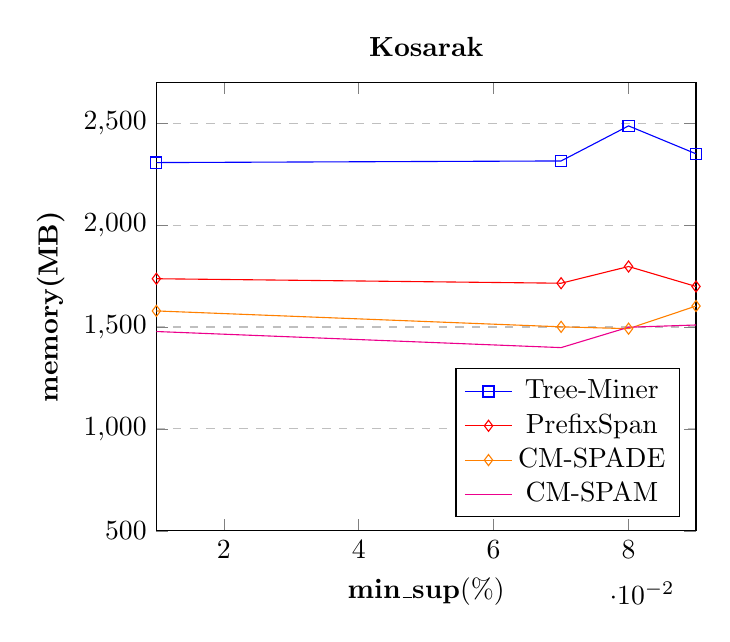
\begin{tikzpicture}
\begin{axis}[
    title={\textbf{Kosarak}},
    xlabel={$\textbf{min\_sup}$(\%)},
    ylabel={\textbf{memory(MB)}},
    xmin=0.01, xmax=0.09,
    ymin=500, ymax=2700,
    %xtick={1200, 1500, 2000},
    %ytick={0,2,4,6,8},
    legend pos=south east,
    ymajorgrids=true,
    grid style=dashed,
]

%(41, 12)
%(47, 9)
%(55, 7)

%tree-miner
\addplot[
    color=blue,
    mark=square,
    ]
    coordinates {
        (0.01, 2307)
        (0.07, 2315)
        (0.08, 2487)
        (0.09, 2350)
    };
    \addlegendentry{Tree-Miner}

  \addplot[
    color=red,
    mark=diamond,
    ]
    coordinates {
        (0.01, 1737)
        (0.07, 1715)
        (0.08, 1797)
        (0.09, 1699)
    };
    \addlegendentry{PrefixSpan}

    \addplot[
        color=orange,
        mark=diamond,
        ]
        coordinates {
            (0.01, 1579)
            (0.07, 1501)
            (0.08, 1492)
            (0.09, 1603)
        };
        \addlegendentry{CM-SPADE}

    \addplot[
    color=magenta
    ]
    coordinates {
        (0.01, 1478)
        (0.07, 1399)
        (0.08, 1499)
        (0.09, 1510)
    };
    \addlegendentry{CM-SPAM}

\end{axis}
\end{tikzpicture}
\end{adjustbox}
\caption{}
\end{subfigure}
        \caption{Memory Comparisons for Tree-Miner}
        \label{graph:memory_comparison_tree_miner}
        \end{figure*}

\begin{table*}[!htbp]
\centering
%% increase table row spacing, adjust to taste
%\renewcommand{\arraystretch}{1.3}
% if using array.sty, it might be a good idea to tweak the value of
% \extrarowheight as needed to properly center the text within the cells
%\centering
%% Some packages, such as MDW tools, offer better commands for making tables
%% than the plain LaTeX2e tabular which is used here.
\begin{tabular}{|l|l|l|l|l|l|l|l|}
\hline
Dataset & Construct- & Mining & $min\_sup$ & $\frac{C}{M}$ & $ M $ & $M$ & $M$ \\
& ion Time  &  Time & (\%) & (\%) & vs & vs & vs\\
& (Sec.) & (Sec.) & & & $Pr$ & $SP$ & $SM$\\
& ($C$) &  ($M$) & & & (\%) & (\%)&(\%)\\
\hline
 Bible & 40 & 2907 & 0.5 & 1.3 & 29  & 20 & 26\\ \hline
 BMSWebView1 & 5 & 1321 &  0.05 & 0.3 & 64 & 52 & 45\\ \hline
 Sign  &  16  &  2448 & 1 & 0.6 & 48 & 28 & 40\\ \hline
 MSNBC & 14 & 3700 & 0.2 & 0.3 & 33 & 18 & 24\\ \hline
 Kosarak & 130 & 7925 & 0.07 & 1.6 & 29 & 22 & 15\\ \hline
L20-C10-T5-N1K & 10 & 1012 & 0.025 & 1 & 56 & 17 & 33\\ \hline
L50-C10-T2.5-N10K & 20 & 2010 & 0.02 & 0.9 & 76 & 64 & 54\\ \hline
\end{tabular}
\caption{Construction Time Vs Mining Time}
\label{table:construction_time_tree_miner}
\end{table*}




\subsection{IncTree-Miner}
In this section, we will analyze the performance of IncTree-Miner based on various metrics.

\subsubsection{Runtime, Memory Usage, Scalability}
Our IncTree-Miner contains all the novelty of Tree-Miner and designs a set of concepts to implicitly track the incremental database which ultimately helps to efficiently mine those patterns which are affected due to the addition of incremental database. It separates the modified and unmodified subtrees, performs projection separately and combines the results to provide the final output. Using modified next links and support count attributes we efficiently detect the modified subtrees and the updated patterns with their changed support. During pattern extensions, first we project in the incremental database and from there using \textit{infrequent to frequent} transition property we first detect which infrequent patterns have chance to be frequent and then decide to perform projection in the remaining database for them. This approach also helps to efficiently update the frequency of the existing frequent patterns which are affected due to the incremental database also leading to the detection of the previously frequent and currently infrequent patterns. We also use BPFSP-Tree as pattern storage which keeps the projection information of the patterns using IncSP-Tree nodes. It reduces the number of DB scans and efficiently removes the infrequent patterns using the bottom-up strategy. It also maintains NIB buffer which makes use of the cost to calculate the support of an infrequent pattern by giving an idea regarding previous support during the following iterations. Sequence Summarizer also helps to incrementally update the co-occurrence information.


In Fig. \ref{graph:runtime_scalability_comparison_inc_tree_miner} (a)-(g), we have shown the runtime performance of IncTree-Miner with $PBIncSpan$ and $IncSP$. From the figure, it is obvious that our proposed algorithm improves runtime by a significant amount. IncSP is based on candidate generation and testing paradigm and it is bound to be slow compared to pattern growth algorithms. PBIncSapn is an efficient solution that follows the pattern growth approach along with applying two efficient pruning mechanisms, width and depth pruning. But these are basically a subset of pruning mechanisms we maintain. PBIncSpan saves the projection information using pseudo projections of the database to reduce the DB scan, whereas we use the compact IncSP-Tree node pointers based BPFSP-Tree for this purpose. Similar to Tree-Miner our performance improvement is quite visible at lower thresholds. As the number of patterns (both frequent and updated) is very small at higher thresholds, the improvement is not much differentiable.

\begin{figure*}[!tb]
        \centering
         \begin{subfigure}{.3\linewidth}
          \centering
           \begin{adjustbox}{max width=\textwidth}
           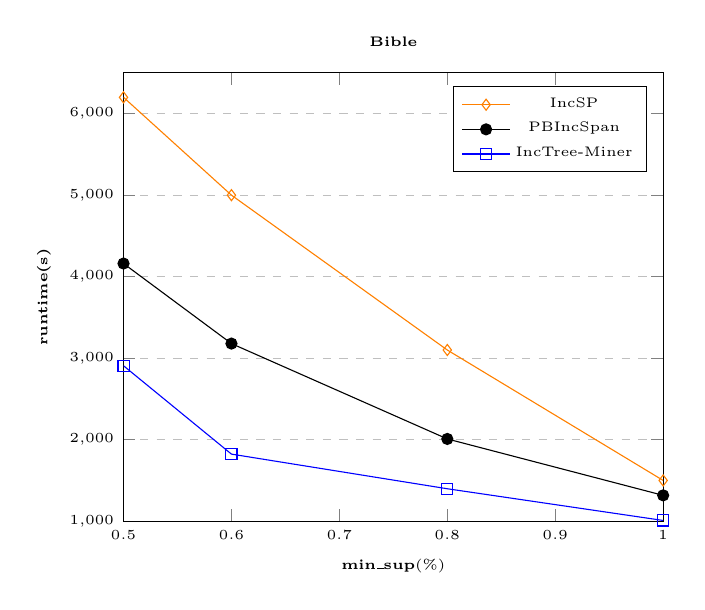
\begin{tikzpicture}
              \begin{axis}[
    title={\textbf{Bible}},
    xlabel={$\textbf{min\_sup}(\%)$},
    ylabel={\textbf{runtime(s)}},
    xmin=0.5, xmax=1,
    ymin=1000, ymax=6500,
    legend pos=north east,
    ymajorgrids=true,
    grid style=dashed,
    legend style={font=\tiny},
    title style={font=\tiny},
    label style={font=\tiny},
    every tick label/.append style={font=\tiny}
]

% (70, 2456.14 * 2.5 = 6140.25)
% (80, 1331.05 * 2.2 = 2928.31)
% (90, 722.725 * 1.8 = 1300.905)
%prefixspan

   \addplot[
    color=orange,
    mark=diamond,
    ]
    coordinates {
        (0.5, 6200)
        (0.6, 5000)
        (0.8, 3100)
        (1, 1500)
    };

   \addlegendentry{IncSP};

   \addplot[
    color=black,
    mark=*,
    ]
    coordinates {
        (0.5, 4161)
        (0.6, 3179)
        (0.8, 2009)
        (1, 1317)
    };
   \addlegendentry{PBIncSpan};

    \addplot[
        color=blue,
        mark=square,
        ]
        coordinates {
            (0.5, 2907)
            (0.6, 1823)
            (0.8, 1398)
            (1,   1009)
        };
   \addlegendentry{IncTree-Miner};
\end{axis}
           \end{tikzpicture}
          \end{adjustbox}
          \caption{}
         \end{subfigure}
        \begin{subfigure}{.3\linewidth}
          \centering
           \begin{adjustbox}{max width=\textwidth}
           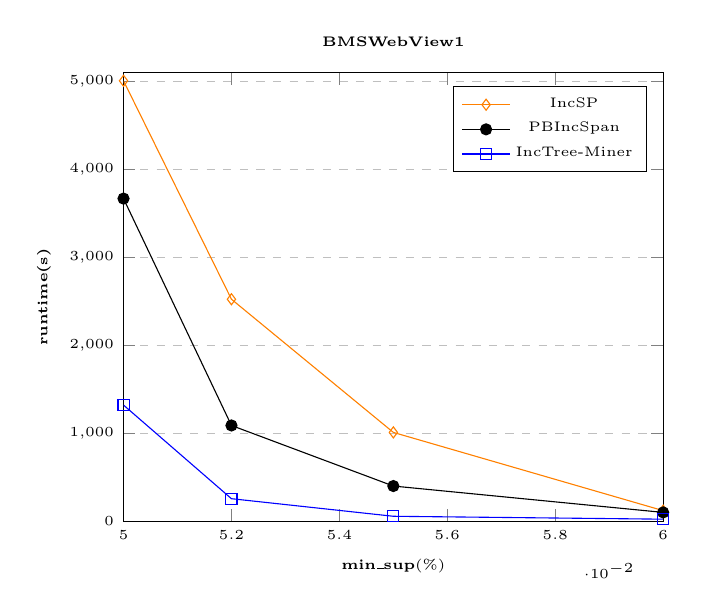
\begin{tikzpicture}
              \begin{axis}[
    title={\textbf{BMSWebView1}},
     xlabel={$\textbf{min\_sup}(\%)$},
    ylabel={\textbf{runtime(s)}},
    xmin=0.05, xmax=0.06,
    ymin=0, ymax=5100,
    legend pos=north east,
    ymajorgrids=true,
    grid style=dashed,
    legend style={font=\tiny},
    title style={font=\tiny},
    label style={font=\tiny},
    every tick label/.append style={font=\tiny}
]
    \addplot[
    color=orange,
    mark=diamond,
    ]
    coordinates {
            (0.06,  120)
            (0.055, 1010)
            (0.052, 2525)
            (0.05,  5010)
    };
    \addlegendentry{IncSP};


    \addplot[
    color=black,
    mark=*,
    ]
    coordinates {
            (0.06,  100)
            (0.055, 400)
            (0.052, 1089)
            (0.05,  3670)
    };

    \addlegendentry{PBIncSpan};

    %tree-miner
    \addplot[
        color=blue,
        mark=square,
        ]
        coordinates {
            (0.06,  23)
            (0.055, 56)
            (0.052, 256)
            (0.05,  1321)
        };
    \addlegendentry{IncTree-Miner};
\end{axis}
           \end{tikzpicture}
          \end{adjustbox}
          \caption{}
         \end{subfigure}
        \begin{subfigure}{.3\linewidth}
          \centering
           \begin{adjustbox}{max width=\textwidth}
           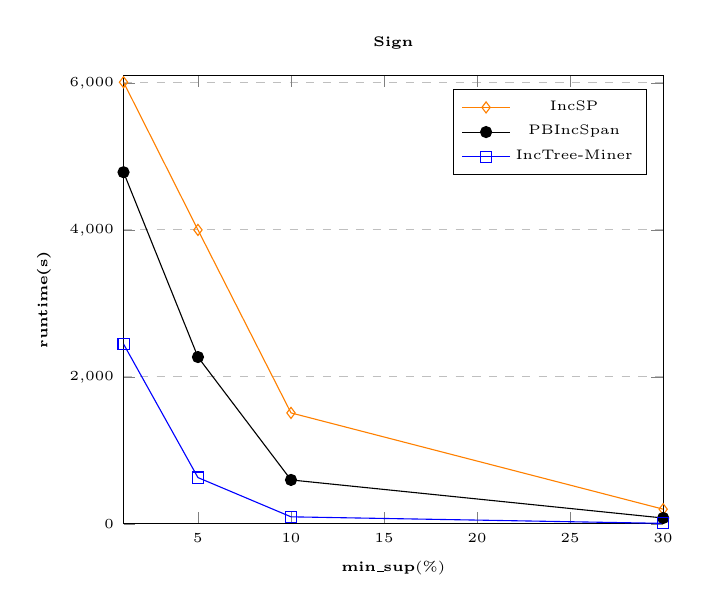
\begin{tikzpicture}
              \begin{axis}[
    title={\textbf{Sign}},
     xlabel={$\textbf{min\_sup}(\%)$},
    ylabel={\textbf{runtime(s)}},
    xmin=1, xmax=30,
    ymin=0, ymax=6100,
    legend pos=north east,
    ymajorgrids=true,
    grid style=dashed,
    legend style={font=\tiny},
    title style={font=\tiny},
    label style={font=\tiny},
    every tick label/.append style={font=\tiny}
]
    \addplot[
    color=orange,
    mark=diamond,
    ]
    coordinates {
            (30, 200)
            (10, 1510)
            (5, 4000)
            (1, 6010)
    };
    \addlegendentry{IncSP}


    \addplot[
    color=black,
    mark=*,
    ]
    coordinates {
            (30, 80)
            (10, 598)
            (5, 2270)
            (1, 4785)
    };
    \addlegendentry{PBIncSpan}
    \addplot[
        color=blue,
        mark=square,
        ]
        coordinates {
            (30, 7)
            (10, 96)
            (5, 630)
            (1, 2448)
        };
   \addlegendentry{IncTree-Miner}
\end{axis}
           \end{tikzpicture}
          \end{adjustbox}
          \caption{}
         \end{subfigure}
        \begin{subfigure}{.3\linewidth}
          \centering
           \begin{adjustbox}{max width=\textwidth}
           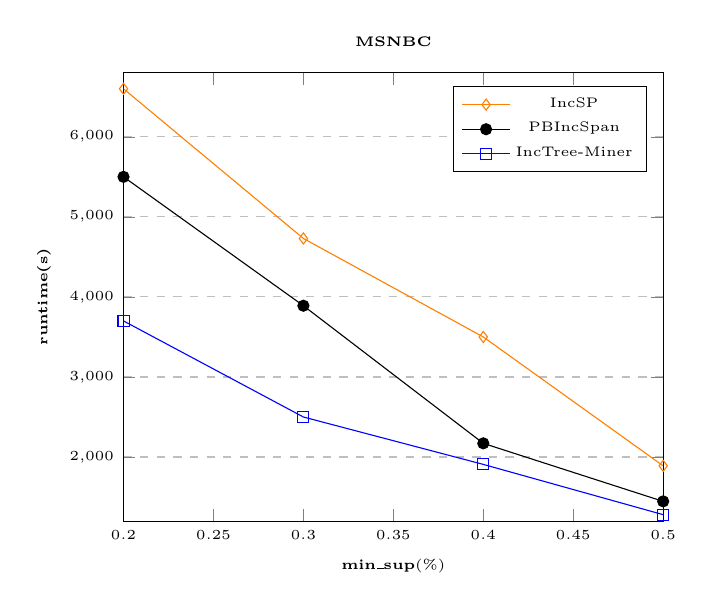
\begin{tikzpicture}
              \begin{axis}[
    title={\textbf{MSNBC}},
    xlabel={$\textbf{min\_sup}(\%)$},
    ylabel={\textbf{runtime(s)}},
    xmin=0.2, xmax=0.5,
    ymin=1200, ymax=6800,
    legend pos=north east,
    ymajorgrids=true,
    grid style=dashed,
    legend style={font=\tiny},
    title style={font=\tiny},
    label style={font=\tiny},
    every tick label/.append style={font=\tiny}
]
    \addplot[
    color=orange,
    mark=diamond,
    ]
    coordinates {
       (0.5, 1890)
       (0.4, 3500)
       (0.3,4730)
       (0.2,6600)
    };
    \addlegendentry{IncSP}

    \addplot[
    color=black,
    mark=*,
    ]
    coordinates {
       (0.5, 1446)
       (0.4, 2171)
       (0.3,3890)
       (0.2,5500)
    };
    \addlegendentry{PBIncSpan}
    %tree-miner
    \addplot[
        color=blue,
        mark=square,
        ]
        coordinates {
            (0.5,1280)
            (0.4,1908)
            (0.3,2500)
            (0.2,3700)
        };
   \addlegendentry{IncTree-Miner}
\end{axis}
           \end{tikzpicture}
          \end{adjustbox}
          \caption{}
         \end{subfigure}
        \begin{subfigure}{.3\linewidth}
          \centering
           \begin{adjustbox}{max width=\textwidth}
           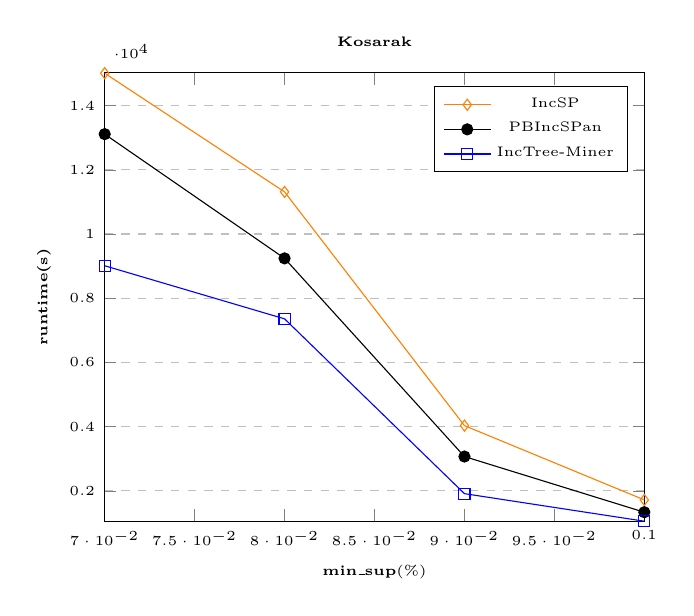
\begin{tikzpicture}
              \begin{axis}[
    title={\textbf{Kosarak}},
     xlabel={$\textbf{min\_sup}(\%)$},
    ylabel={\textbf{runtime(s)}},
    xmin=0.07, xmax=0.1,
    ymin=1055, ymax=15020,
    legend pos=north east,
    ymajorgrids=true,
    grid style=dashed,
    legend style={font=\tiny},
    title style={font=\tiny},
    label style={font=\tiny},
    every tick label/.append style={font=\tiny}
]
    \addplot[
    color=orange,
    mark=diamond,
    ]
    coordinates {
            (0.1, 1718)
            (0.09, 4032)
            (0.08, 11312)
            (0.07, 15010)
    };
    \addlegendentry{IncSP}

    \addplot[
    color=black,
    mark=*,
    ]
    coordinates {
            (0.1, 1335)
            (0.09, 3069)
            (0.08, 9242)
            (0.07, 13112)
    };
    \addlegendentry{PBIncSPan}

    \addplot[
        color=blue,
        mark=square,
        ]
        coordinates {
            (0.1, 1055)
            (0.09, 1913)
            (0.08, 7358)
            (0.07, 9012)
        };
    \addlegendentry{IncTree-Miner}
\end{axis}
           \end{tikzpicture}
          \end{adjustbox}
          \caption{}
         \end{subfigure}
       \begin{subfigure}{.3\linewidth}
          \centering
           \begin{adjustbox}{max width=\textwidth}
           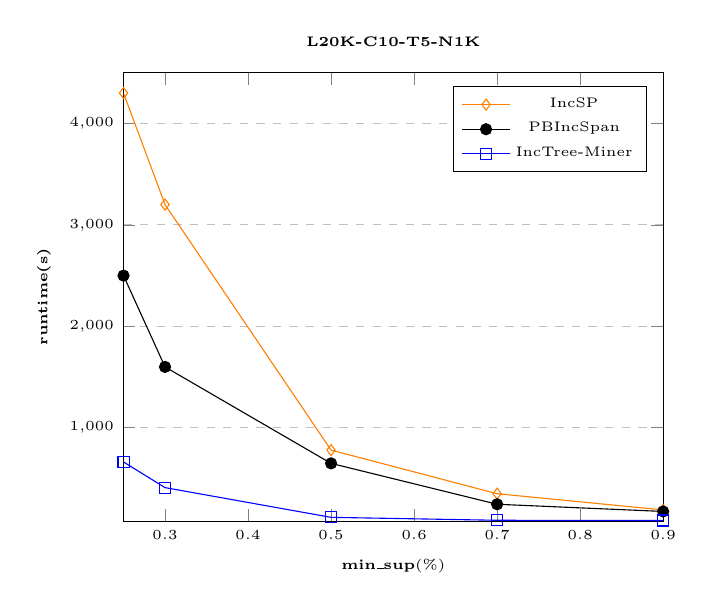
\begin{tikzpicture}
              \begin{axis}[
    title={\textbf{L20K-C10-T5-N1K}},
     xlabel={$\textbf{min\_sup}(\%)$},
    ylabel={\textbf{runtime(s)}},
    xmin=0.25, xmax=0.9,
    ymin=80, ymax=4500,
    legend pos=north east,
    ymajorgrids=true,
    grid style=dashed,
    legend style={font=\tiny},
    title style={font=\tiny},
    label style={font=\tiny},
    every tick label/.append style={font=\tiny}
]

\addplot[
    color=orange,
    mark=diamond,
    ]
    coordinates {
            (0.9, 190)
            (0.7, 350)
            (0.5, 780)
            (0.3, 3200)
            (0.25, 4300)
    };
    \addlegendentry{IncSP}

    \addplot[
    color=black,
    mark=*,
    ]
    coordinates {
            (0.9, 175)
            (0.7, 246)
            (0.5, 649)
            (0.3,  1600)
            (0.25, 2500)
    };
    \addlegendentry{PBIncSpan}

    %tree-miner
    \addplot[
        color=blue,
        mark=square,
        ]
        coordinates {
            (0.9, 86)
            (0.7, 88)
            (0.5, 117)
            (0.3,  410)
            (0.25, 663)
        };
   \addlegendentry{IncTree-Miner}
\end{axis}
           \end{tikzpicture}
          \end{adjustbox}
          \caption{}
         \end{subfigure}
      \begin{subfigure}{.3\linewidth}
          \centering
           \begin{adjustbox}{max width=\textwidth}
           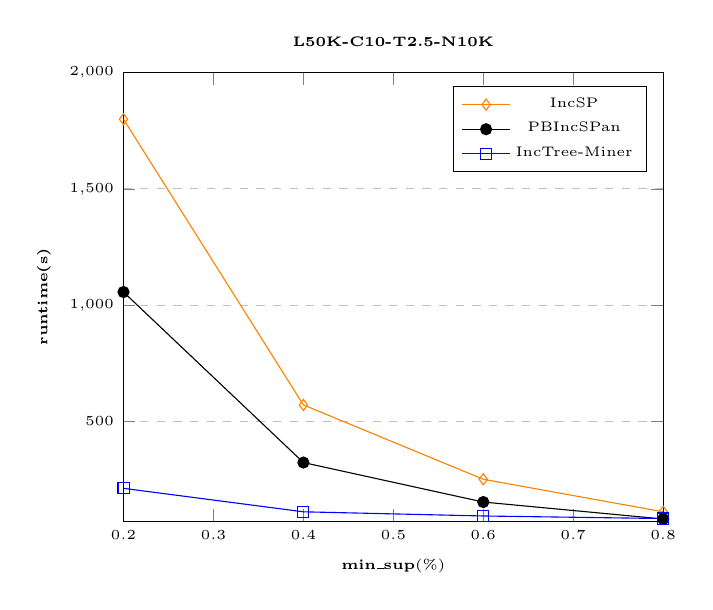
\begin{tikzpicture}
              \begin{axis}[
    title={\textbf{L50K-C10-T2.5-N10K}},
     xlabel={$\textbf{min\_sup}(\%)$},
    ylabel={\textbf{runtime(s)}},
    xmin=0.2, xmax=0.8,
    ymin=70, ymax=2000,
    legend pos=north east,
    ymajorgrids=true,
    grid style=dashed,
    legend style={font=\tiny},
    title style={font=\tiny},
    label style={font=\tiny},
    every tick label/.append style={font=\tiny}
]
    \addplot[
    color=orange,
    mark=diamond,
    ]
    coordinates {
        (0.8, 110)
        (0.6, 250)
        (0.4, 570)
        (0.2, 1800)
    };
    \addlegendentry{IncSP}

    \addplot[
    color=black,
    mark=*,
    ]
    coordinates {
            (0.8, 79)
            (0.6, 152)
            (0.4, 322)
            (0.2,  1056)
    };
    \addlegendentry{PBIncSPan}

    \addplot[
        color=blue,
        mark=square,
        ]
        coordinates {
            (0.8, 81)
            (0.6, 92)
            (0.4, 110)
            (0.2,  211)
        };
    \addlegendentry{IncTree-Miner}
\end{axis}
           \end{tikzpicture}
          \end{adjustbox}
          \caption{}
         \end{subfigure}
          \begin{subfigure}{.3\linewidth}
          \begin{adjustbox}{max width=\textwidth}
          \centering
          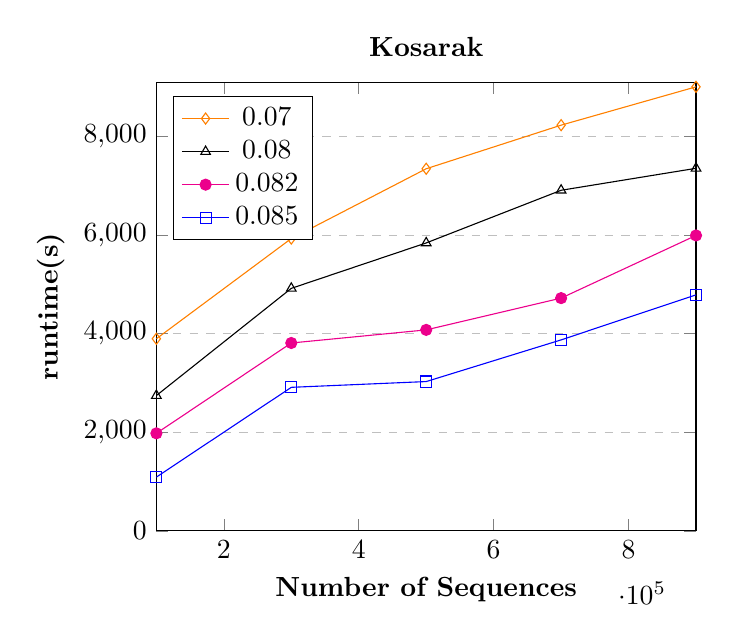
\begin{tikzpicture}
            \begin{axis}[
            title={\textbf{Kosarak}},
            xlabel={\textbf{Number of Sequences}},
            ylabel={\textbf{runtime(s)}},
            xmin=100000, xmax=900000,
            ymin=0, ymax=9100,
            legend pos=north west,
            ymajorgrids=true,
            grid style=dashed,
        ]
            \addplot[
            color=orange,
            mark=diamond,
            ]
            coordinates {
                  (900000,9012)
                  (700000,8234)
                  (500000,7349)
                  (300000,5932)
                  (100000,3898)
            };
            \addplot[
            color=black,
            mark=triangle
            ]
            coordinates {
                  (900000,7358)
                  (700000,6912)
                  (500000,5843)
                  (300000,4921)
                  (100000,2745)
            };
            \addplot[
            color=magenta,
            mark=*,
            ]
            coordinates {
                  (900000,5995)
                  (700000,4723)
                  (500000,4078)
                  (300000,3812)
                  (100000,1978)
            };
            \addplot[
                color=blue,
                mark=square,
                ]
                coordinates {
                  (900000,4789)
                  (700000,3875)
                  (500000,3029)
                  (300000,2912)
                  (100000,1090)
                };
            \legend{0.07, 0.08, 0.082, 0.085}
        \end{axis}
         \end{tikzpicture}
          \end{adjustbox}
          \caption{}
           \end{subfigure}
         \caption{(a)-(g): Runtime Comparison, (h) Scalability Comparisons for IncTree-Miner}
        \label{graph:runtime_scalability_comparison_inc_tree_miner}
\end{figure*}

\textcolor{blue}{Upto now, we have compared with the base proposals related to incremental mining that aligns with the motivation of the proposed solution. Now, we will provide some analysis through comparing with a prominent literature that does not completely aligns with the motivation of the proposed work but goes closely with it, to understand our solution's efficacy in improving runtime.}

\textcolor{blue}{For the comparison MR-INCSPM\cite{saleti2019mapreduce} has been chosen, a Map Reduced framework for ISPM problems. As the proposed solution works for a single machine environment, here for MR-INCSPM such environment has been considered for fair ground analysis. MR-INCSPM worked in backward extension with its own co-occurrence table definition and pruning strategies. So, these factors also provided important points to conduct a critical analysis.}

\textcolor{blue}{In Fig.\ref{figure:mr_incspm}, we have shown the results for some of the datasets. From the figures, it can be noted that, the performance of IncTree-Miner is comparatively better. The main issue, in single machine based MR-INCSPM is, it generates patterns with sort of prefixspan or database projection alike technique but with backward extension. Here the main improvement factor of ours is faster traversal through links compared to scan based moves. Alongside, their proposed pruning strategies are a subset of the strategies we use for our pruning. So, altogether the performance improvement is achieved.}

\textcolor{blue}{In \cite{lin2015incrementally}, pre-large concept was proposed where additional set of patterns which are not exactly frequent are pre-computed, so that the number of database re-scans can be reduced. There the authors use additional set of thresholds, upper($s_{u}$) and lower($s_{l}$) minimum support thresholds to perform the additional patterns' pre-computation. The performance of database re-scans can be improved using the proposed IncSP-Tree structure through using its next links and modified next links. These over-computation based approaches suffer greatly when concept drift appears along with the critical selection of the empirically set thresholds.}

\begin{figure*}[!tb]
        \centering
        \begin{subfigure}{.3\linewidth}
          \centering
           \begin{adjustbox}{max width=\textwidth}
           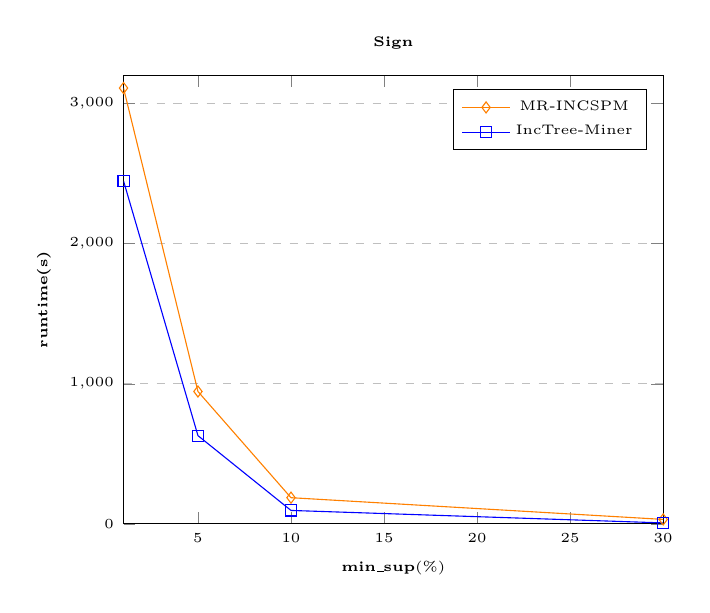
\begin{tikzpicture}
              \begin{axis}[
    title={\textbf{Sign}},
     xlabel={$\textbf{min\_sup}(\%)$},
    ylabel={\textbf{runtime(s)}},
    xmin=1, xmax=30,
    ymin=0, ymax=3200,
    legend pos=north east,
    ymajorgrids=true,
    grid style=dashed,
    legend style={font=\tiny},
    title style={font=\tiny},
    label style={font=\tiny},
    every tick label/.append style={font=\tiny}
]
    \addplot[
    color=orange,
    mark=diamond,
    ]
    coordinates {
            (30, 32)
            (10, 187)
            (5, 945)
            (1, 3111)
    };
    \addlegendentry{MR-INCSPM}

    \addplot[
        color=blue,
        mark=square,
        ]
        coordinates {
            (30, 7)
            (10, 96)
            (5, 630)
            (1, 2448)
        };
   \addlegendentry{IncTree-Miner}
\end{axis}
           \end{tikzpicture}
          \end{adjustbox}
          \caption{}
         \end{subfigure}
        \begin{subfigure}{.3\linewidth}
          \centering
           \begin{adjustbox}{max width=\textwidth}
           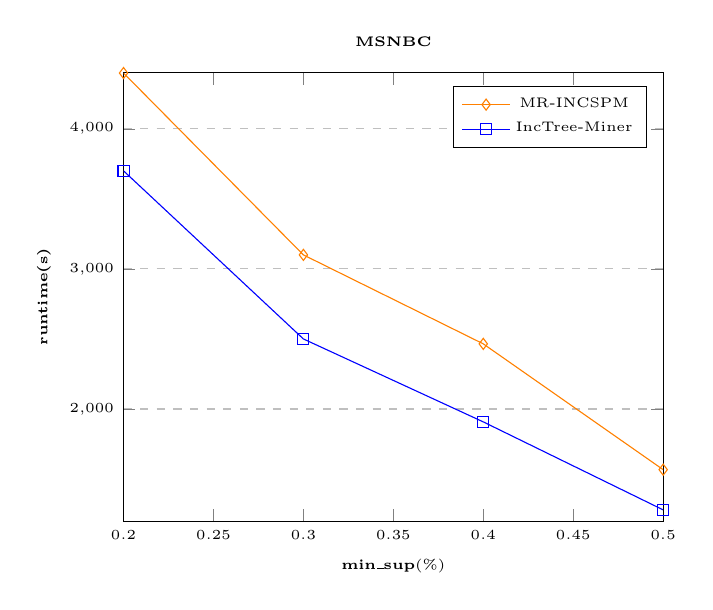
\begin{tikzpicture}
              \begin{axis}[
    title={\textbf{MSNBC}},
    xlabel={$\textbf{min\_sup}(\%)$},
    ylabel={\textbf{runtime(s)}},
    xmin=0.2, xmax=0.5,
    ymin=1200, ymax=4400,
    legend pos=north east,
    ymajorgrids=true,
    grid style=dashed,
    legend style={font=\tiny},
    title style={font=\tiny},
    label style={font=\tiny},
    every tick label/.append style={font=\tiny}
]
    \addplot[
    color=orange,
    mark=diamond,
    ]
    coordinates {
       (0.5, 1567)
       (0.4, 2465)
       (0.3,3100)
       (0.2,4398)
    };
    \addlegendentry{MR-INCSPM}

    %tree-miner
    \addplot[
        color=blue,
        mark=square,
        ]
        coordinates {
            (0.5,1280)
            (0.4,1908)
            (0.3,2500)
            (0.2,3700)
        };
   \addlegendentry{IncTree-Miner}
\end{axis}
           \end{tikzpicture}
          \end{adjustbox}
          \caption{}
         \end{subfigure}
        \begin{subfigure}{.3\linewidth}
          \centering
           \begin{adjustbox}{max width=\textwidth}
           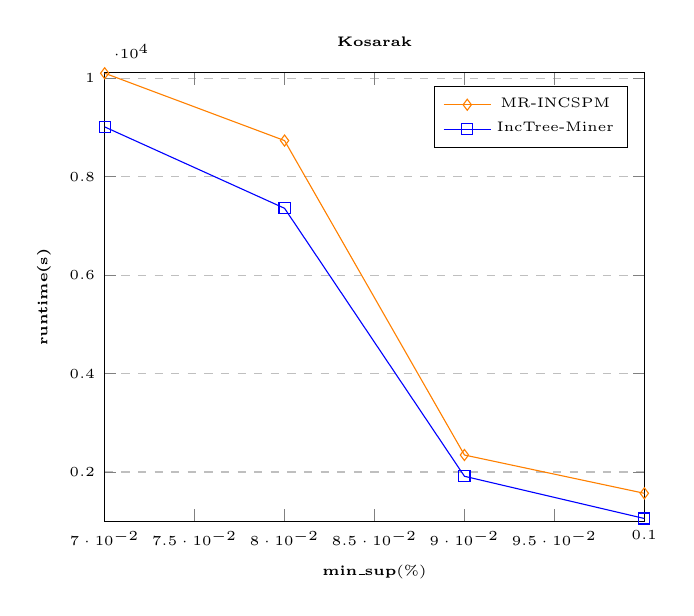
\begin{tikzpicture}
              \begin{axis}[
    title={\textbf{Kosarak}},
     xlabel={$\textbf{min\_sup}(\%)$},
    ylabel={\textbf{runtime(s)}},
    xmin=0.07, xmax=0.1,
    ymin=1000, ymax=10110,
    legend pos=north east,
    ymajorgrids=true,
    grid style=dashed,
    legend style={font=\tiny},
    title style={font=\tiny},
    label style={font=\tiny},
    every tick label/.append style={font=\tiny}
]
    \addplot[
    color=orange,
    mark=diamond,
    ]
    coordinates {
            (0.1, 1567)
            (0.09, 2345)
            (0.08, 8734)
            (0.07, 10103)
    };
    \addlegendentry{MR-INCSPM}

    \addplot[
        color=blue,
        mark=square,
        ]
        coordinates {
            (0.1, 1055)
            (0.09, 1913)
            (0.08, 7358)
            (0.07, 9012)
        };
    \addlegendentry{IncTree-Miner}
\end{axis}
           \end{tikzpicture}
          \end{adjustbox}
          \caption{}
         \end{subfigure}
         \caption{Runtime Comparison with MR-INCSPM}
        \label{figure:mr_incspm}
\end{figure*}


\begin{figure*}[!thb]
        \centering
       \begin{subfigure}{.3\textwidth}
          \centering
           \begin{adjustbox}{max width=\textwidth}
           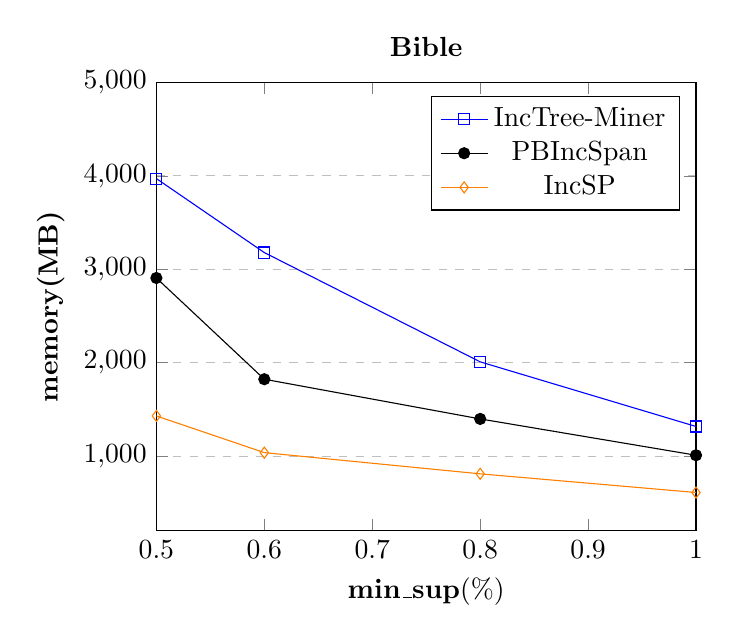
\begin{tikzpicture}
              \begin{axis}[
    title={\textbf{Bible}},
    xlabel={$\textbf{min\_sup}(\%)$},
    ylabel={\textbf{memory(MB)}},
    xmin=0.5, xmax=1,
    ymin=200, ymax=5000,
    legend pos=north east,
    ymajorgrids=true,
    grid style=dashed,
]

% (70, 2456.14 * 2.5 = 6140.25)
% (80, 1331.05 * 2.2 = 2928.31)
% (90, 722.725 * 1.8 = 1300.905)
%prefixspan
    \addplot[
    color=blue,
    mark=square,
    ]
    coordinates {
        (0.5, 3971)
        (0.6, 3179)
        (0.8, 2009)
        (1, 1317)
    };
    \addlegendentry{IncTree-Miner}
    %tree-miner
    \addplot[
        color=black,
        mark=*,
        ]
        coordinates {
            (0.5, 2907)
            (0.6, 1823)
            (0.8, 1398)
            (1,   1009)
        };
    \addlegendentry{PBIncSpan}

    \addplot[
        color=orange,
        mark=diamond,
        ]
        coordinates {
            (0.5, 1430)
            (0.6, 1037)
            (0.8, 810)
            (1,   610)
        };
    \addlegendentry{IncSP}
\end{axis}
           \end{tikzpicture}
          \end{adjustbox}
          \caption{}
         \end{subfigure}
        \begin{subfigure}{.3\textwidth}
          \centering
           \begin{adjustbox}{max width=\textwidth}
           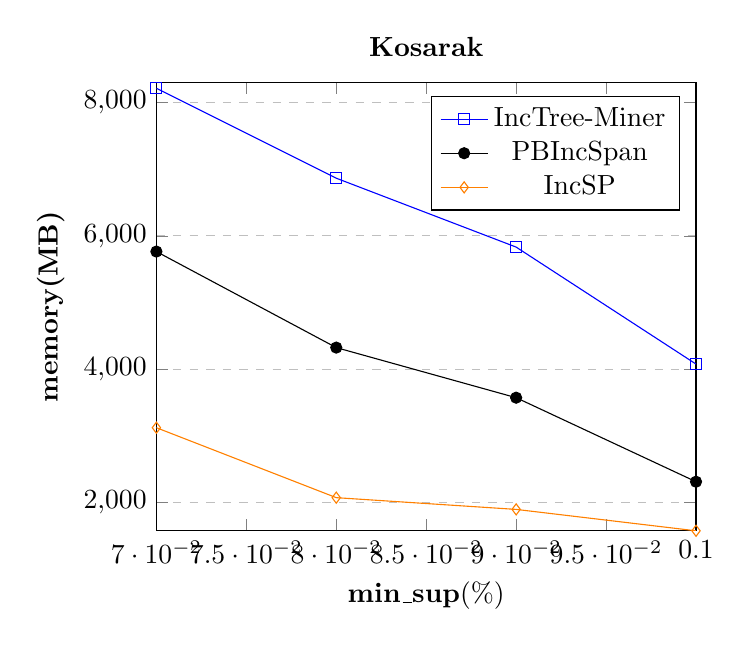
\begin{tikzpicture}
              \begin{axis}[
    title={\textbf{Kosarak}},
    xlabel={$\textbf{min\_sup}(\%)$},
    ylabel={\textbf{memory(MB)}},
    xmin=0.07, xmax=0.1,
    ymin=1578, ymax=8300,
    legend pos=north east,
    ymajorgrids=true,
    grid style=dashed,
]

% (70, 2456.14 * 2.5 = 6140.25)
% (80, 1331.05 * 2.2 = 2928.31)
% (90, 722.725 * 1.8 = 1300.905)
%prefixspan
    \addplot[
    color=blue,
    mark=square,
    ]
    coordinates {
        (0.1, 4078)
        (0.09, 5832)
        (0.08, 6865)
        (0.07, 8214)
    };
    \addlegendentry{IncTree-Miner}
    %tree-miner
    \addplot[
        color=black,
        mark=*,
        ]
        coordinates {
            (0.1, 2314)
            (0.09, 3574)
            (0.08, 4325)
            (0.07, 5765)
        };
    \addlegendentry{PBIncSpan}

    \addplot[
        color=orange,
        mark=diamond,
        ]
        coordinates {
            (0.1, 1578)
            (0.09, 1899)
            (0.08, 2075)
            (0.07, 3124)
        };
    \addlegendentry{IncSP}
\end{axis}
           \end{tikzpicture}
          \end{adjustbox}
          \caption{}
         \end{subfigure}
         \begin{subfigure}{.3\textwidth}
          \centering
           \begin{adjustbox}{max width=\textwidth}
           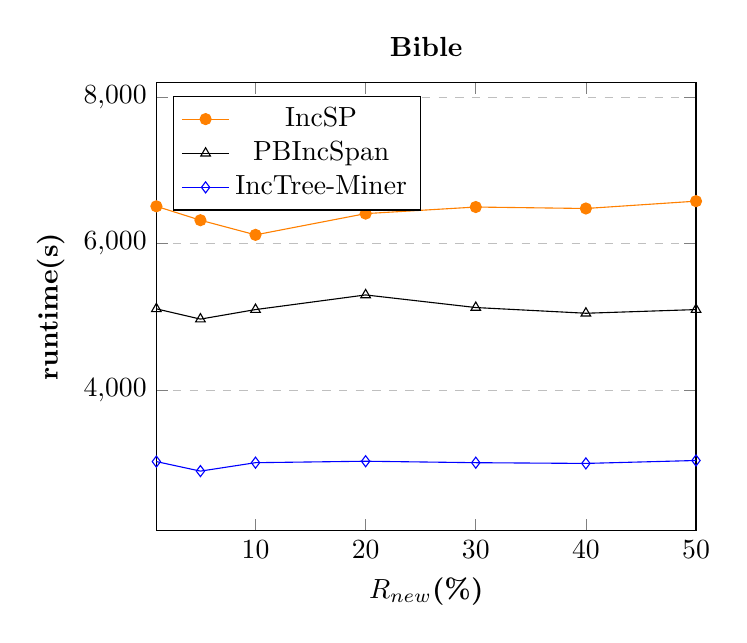
\begin{tikzpicture}
              \begin{axis}[
    title={\textbf{Bible}},
    xlabel={\textbf{$R_{new}$(\%)}},
    ylabel={\textbf{runtime(s)}},
    xmin=1, xmax=50,
    ymin=2080, ymax=8200,
    legend pos=north west,
    ymajorgrids=true,
    grid style=dashed,
]

 \addplot[
    color=orange,
    mark=*,
    ]
    coordinates {
        (1,6510)
        (5,6320)
        (10,6120)
        (20,6410)
        (30,6500)
        (40,6480)
        (50,6580)
    };
    \addlegendentry{IncSP}

  \addplot[
    color=black,
    mark=triangle,
    ]
    coordinates {
        (1,5110)
        (5,4970)
        (10,5100)
        (20,5300)
        (30,5128)
        (40,5050)
        (50,5100)
    };
    \addlegendentry{PBIncSpan}

   \addplot[
    color=blue,
    mark=diamond
    ]
    coordinates {
         (1,3025)
         (5,2895)
         (10,3010)
         (20,3030)
         (30,3010)
         (40,3000)
         (50,3040)
    };
    \addlegendentry{IncTree-Miner}
\end{axis}
           \end{tikzpicture}
          \end{adjustbox}
          \caption{}
         \end{subfigure}
         \caption{(a)-(b) Memory Evaluation, (c) Performance over $R_{new}$, for IncTree-Miner}
        \label{graph:memory_rnew_comparison_inctree_miner}
\end{figure*}

ISPM algorithms generally need more memory compared to static mining algorithms because they store the frequent patterns' information which is used in the successive iterations. We show a memory usage analysis in Fig. \ref{graph:memory_rnew_comparison_inctree_miner} (a)-(b) over Bible and Kosarak dataset. IncSP stores the support of the prior frequent patterns. So, its memory usage is dependent on the number of frequent patterns. PBIncSpan and IncTree-Miner both keep the previous frequent patterns' support along with their projection information where PBIncSpan uses pseudo projection and IncTree-Miner uses the compact IncSP-Tree node references. But IncTree-Miner stores the sequential database in tree format along with maintaining some data structures leading to comparatively more memory usage than PBIncSpan. As memory usage is directly related to the compactness of the tree, so in dense datasets, this metric's performance is comparatively closer to PBIncSpan. Our incremental solution is the extension of prior proposed static solution and both maintain almost similar types of data structures. In the earlier section, we have discussed how this additional usage gives us significant improvement in mining which also applies here. Being very flexible solution, we have our own memory resilient version. In the memory resilient version, we do not store pattern's projection information which reduces the memory to a great extent with additional time cost during mining.

Similar to Tree-Miner, we also conducted a scalability test for IncTree-Miner and presented the result over the \textit{Kosarak} dataset in Fig. \ref{graph:runtime_scalability_comparison_inc_tree_miner} (h). We started with few transactions, gradually increased it and recorded the results by varying $min\_sup$. The corresponding figure shows the linear scalability of the solution. To conduct the experiment, we chose $R_{new}=10\%,R_{com}=50\%$ and $R_{prev}=80\%$ over the considered number of transactions. In the Tree-Miner section, we have shown that the structural solution does not create a bottleneck to construct them rather provides improvement in mining time. As IncSP-Tree is an incremental version of SP-Tree it also maintains similar characteristics.




%Link: https://tex.stackexchange.com/questions/249085/referencing-subfigures-with-subfigure-package

\subsubsection{Effect on Different $R_{new}$ and $R_{com}$}

To evaluate the performance over the ratio of the completely new sequences (new sids) we conducted experiment by varying the percentage of $R_{new}$ over $Bible$ dataset by keeping $R_{com}=50\%$, $R_{prev}=80\%$ and $min\_sup=0.3\%$. We have shown the result in Fig. \ref{graph:memory_rnew_comparison_inctree_miner} (c). We started with $1\%$ and gradually increased it to $30\%$ and we always had two iterations to output the final set of patterns. We wanted to observe if the increased ratio of $R_{new}$ affects the solution's performance or not. From Fig. \ref{graph:memory_rnew_comparison_inctree_miner} (c) it is clear that IncTree-Miner's performance does not degrade due to the $R_{new}$'s increasing ratio compared to PBIncSpan and IncSP. With $R_{new}$'s increment the number of newer patterns' and updated patterns' get increased in the second pass and the number of frequent patterns' get decreased in the first pass. So, in our described scenario, the ISPM algorithm's performance should be almost linear and Fig. \ref{graph:memory_rnew_comparison_inctree_miner} (c) supports our intuition.



Similar to $R_{new}$, we also evaluated our solution by changing the percentage of $R_{com}$. For experiment, we had set $R_{new}=10\%, R_{prev}=80\%$ and varied $R_{com}$ with $min\_sup=0.5\%$. Like the previous discussion, we got almost similar types of results which matched our intuition that IncTree-Miner is not affected due to the increment of the $R_{com}$ and performs comparatively better than PBIncSpan and IncSP.






\subsection{Evaluation of Breadth-First Based Support Counting Technique}

\begin{figure*}[ht]
        \centering
            \begin{adjustbox}{max width=1\textwidth}
             \centering
           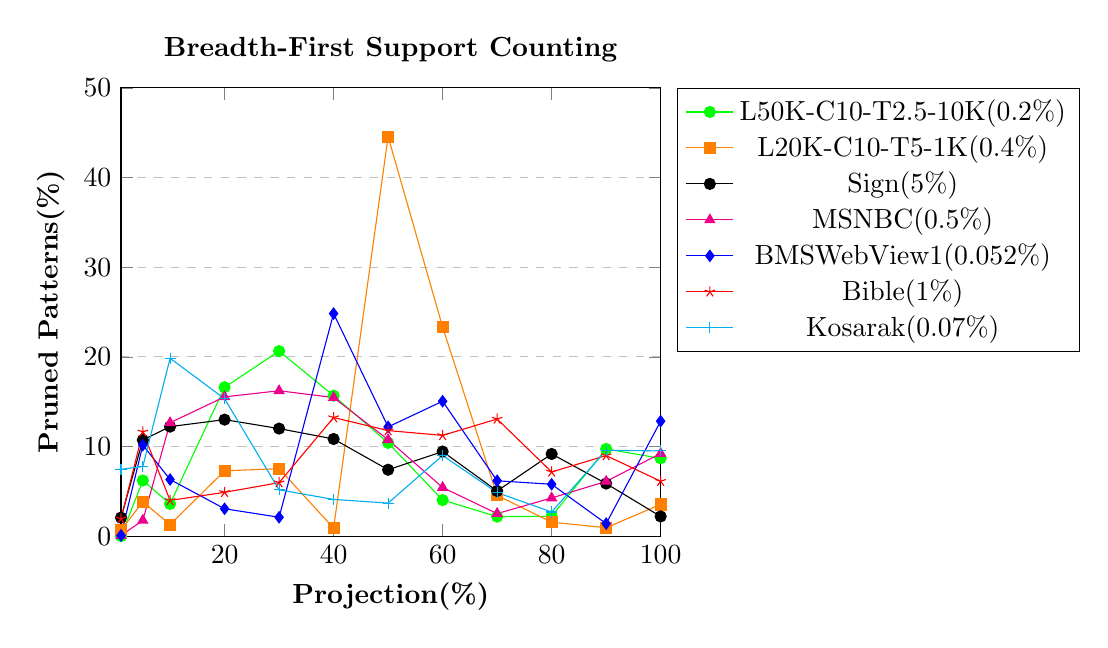
\begin{tikzpicture}
              \begin{axis}[
    title={\textbf{Breadth-First Support Counting}},
    xlabel={\textbf{Projection(\%)}},
    ylabel={\textbf{Pruned Patterns(\%)}},
    xmin=1, xmax=100,
    ymin=0, ymax=50,
    legend pos= outer north east,
    ymajorgrids=true,
    grid style=dashed,
]

\addplot [
    color=green,
    mark=*
    ]
    coordinates {
    (1,0.01)
    (5,6.21)
    (10,3.6)
    (20,16.61)
    (30,20.64)
    (40,15.67)
    (50,10.41)
    (60,4.03)
    (70,2.18)
    (80,2.22)
    (90,9.73)
    (100,8.68)
    };
    \addlegendentry{L50K-C10-T2.5-10K(0.2\%)}

 \addplot [
    color=orange,
    mark=square*
    ]
    coordinates {
    (1,0.67)
    (5,3.84)
    (10,1.29)
    (20,7.29)
    (30,7.53)
    (40,0.9)
    (50,44.56)
    (60,23.32)
    (70,4.55)
    (80,1.56)
    (90,0.95)
    (100,3.54)
    };
    \addlegendentry{L20K-C10-T5-1K(0.4\%)}

    \addplot [
    color=black,
    mark=otimes*
    ]
    coordinates {
      (1,2.07)
    (5,10.73)
    (10,12.22)
    (20,13.0)
    (30,12.0)
    (40,10.84)
    (50,7.41)
    (60,9.44)
    (70,5.04)
    (80,9.17)
    (90,5.87)
    (100,2.2)
    };
    \addlegendentry{Sign(5\%)}

    \addplot [
    color=magenta,
    mark=triangle*
    ]
    coordinates {
        (1,0.07)
        (5,1.77)
        (10,12.65)
        (20,15.54)
        (30,16.22)
        (40,15.46)
        (50,10.76)
        (60,5.43)
        (70,2.52)
        (80,4.26)
        (90,6.11)
        (100,9.22)
    };
    \addlegendentry{MSNBC(0.5\%)}

    \addplot [
    color=blue,
    mark=diamond*
    ]
    coordinates {
        (1,0.09)
        (5,10.16)
        (10,6.32)
        (20,3.06)
        (30,2.11)
        (40,24.83)
        (50,12.19)
        (60,15.05)
        (70,6.18)
        (80,5.79)
        (90,1.4)
        (100,12.83)
    };
    \addlegendentry{BMSWebView1(0.052\%)}

    \addplot [
        color=red,
        mark=star
        ]
        coordinates {
         (1,1.93)
        (5,11.64)
        (10,3.99)
        (20,4.89)
        (30,5.97)
        (40,13.23)
        (50,11.78)
        (60,11.24)
        (70,13.07)
        (80,7.16)
        (90,8.99)
        (100,6.13)
        };
        \addlegendentry{Bible(1\%)}
        \addplot [
        color=cyan,
        mark=+
        ]
        coordinates {
        (1,7.46)
        (5,7.77)
        (10,19.84)
        (20,15.33)
        (30,5.17)
        (40,4.1)
        (50,3.69)
        (60,9.0)
        (70,4.86)
        (80,2.7)
        (90,9.58)
        (100,9.51)
        };
        \addlegendentry{Kosarak(0.07\%)}
\end{axis}
           \end{tikzpicture}
           \end{adjustbox}
         \caption{Evaluation of Breadth-First Based Support Counting Technique}
        \label{graph:breadth-first-support}
\end{figure*}

In this section, we will evaluate the performance of the proposed breadth-first based support counting technique to understand how fast it can detect an infrequent pattern and stop support counting. To guide our mining process we use the co-occurrence information of the items stored in $sList$ and $iList$. With the suffix extension of the pattern these two lists shrink. During support calculation of the extensions, we discover some patterns' infrequency. The algorithm's runtime improves depending on how quickly it is able to detect the infrequency rather than performing complete projection. In Fig. \ref{graph:breadth-first-support}, we present an analysis to understand how quickly our proposed pruning technique detects infrequent patterns. In the x-axis, we have provided the percentage value of the projection size and in the y-axis, we have provided the percentage of infrequent patterns been detected. For example, in the \textit{L20-C10-T2.5-10K} dataset, at 50\% value in the x-axis, we get a 45\% value in the corresponding y-axis, which denotes that, of all the infrequent patterns been tested, 45\% of them are detected performing only 50\% projection of their corresponding complete projected database. From, Fig. \ref{graph:breadth-first-support}, it is clear that our proposed support counting technique is able to detect most of the infrequent patterns without performing a complete projection of the underlying sub-database. We have shown the corresponding $min\_sup$ values beside each legend in Fig. \ref{graph:breadth-first-support}.  The figure is generated by executing Tree-Miner.



\subsection{Effectiveness in Interactive Mining}
The proposed SP-Tree structures hold ``build-once-mine-many" property which states that the structures are capable of performing multiple mining iterations based on users' requests without bringing any change to the existing structures for different $min\_sup$ values.

The most difficult scenario in interactive mining is, the gradual decrease in $min\_sup$  ($20\% \,\to\, 10\% \,\to\, 5\%$, etc) where with this decrease a new set of previously infrequent patterns may become frequent. So, to discover those patterns, we need to perform a mining iteration. Here, using BPFSP-Tree's patterns' projection information we can efficiently discover the newly frequent patterns which will be the super patterns (apriori property) of existing frequent patterns. Through projection information, we can directly reach a pattern's corresponding nodes and start expanding from there using the next links. In Table \ref{table:interactive_mining_descending_minsup}(second group of column) we have shown some results related to this scenario. If, we had to start mining from scratch then the time usage would have increased significantly. Here the mining time gets reduced because already a group of patterns have been calculated alongside can use projection information and faster pattern search procedure.

\begin{table*}[!htbp]
\centering
%% increase table row spacing, adjust to taste
%\renewcommand{\arraystretch}{1.3}
% if using array.sty, it might be a good idea to tweak the value of
% \extrarowheight as needed to properly center the text within the cells
%\centering
%% Some packages, such as MDW tools, offer better commands for making tables
%% than the plain LaTeX2e tabular which is used here.
\begin{tabular}{|l|l|l|l|l|l|l|l|l|l|}
\hline
 Dataset & \multicolumn{5}{l|}{Descending $min\_sup$}  & \multicolumn{4}{l|}{Ascending $min\_sup$} \\
 \hline
 Bible & $min\_sup(\%)$ & 10 & 1 & 0.8 & 0.5 & 0.5 & 0.8 & 1 & 5\\
 & T(sec.) & 228.2 & 579.2 & 675 & 935.5 &  2907 & 0.0008 & 0.0007 & 0.0003\\
 \hline
 BMSWebView1 & $min\_sup(\%)$ & 0.06 & 0.055 & 0.052 & 0.05 & 0.05 & 0.052 & 0.055 & 0.06 \\
 & T(sec.) & 19.8 & 71 & 226.5 & 865.2 & 1321 & 5.7 & 1.1 & 0.7  \\
 \hline
 Sign & $min\_sup(\%)$ & 30 & 10 & 5 & 1 & 1  & 5 & 10 & 30 \\
 & T(sec.) & 19.8 & 71 & 226.5 & 865.2 & 1 & 5 & 10 & 30 \\
 \hline
 MSNBC & $min\_sup(\%)$ &  0.085 & 0.08 & 0.075 & 0.07 & 0.2 & 0.3 & 0.35 & 0.4 \\
 & T(sec.) & 1037.4 & 492.7 & 829 & 742.2 & 3700 & 0.4 & 0.3 & 0.2 \\
 \hline
 Kosarak & $min\_sup(\%)$ &0.085 & 0.08 & 0.075 & 0.07 & 0.07 & 0.075 & 0.08 & 0.085\\
 & T(sec.) & 3037.3 & 2512 & 1231.4 & 1021.3 & 7925 & 5.1 & 3.05 &0.98 \\
 \hline
 L20-C10-T5-N1K & $min\_sup(\%)$ & 0.04 & 0.035 & 0.03 & 0.025  & 0.025 & 0.03 & 0.035 & 0.04 \\
 & T(sec.) & 313.7 & 221.5 & 325.3 & 710 & 1012 & 1.14 & 0.08 & 0.07 \\
 \hline
 L50-C10-T2.5-N10K & $min\_sup(\%)$ & 0.031 & 0.03 & 0.025 & 0.02 & 0.02 & 0.025 & 0.03 & 0.031 \\
 & T(sec.) & 313.7 & 221.5 & 325.3 & 710 & 2010 & 0.2 & 0.11 & 0.05 \\
 \hline
\end{tabular}
\caption{Interactive Mining: Performance in Descending $min\_sup$ and Ascending $min\_sup$.}
\label{table:interactive_mining_descending_minsup}
\end{table*}

The best case scenario, in interactive mining comes from the gradual increase in $min\_sup$ ($5\% \,\to\, 10\% \,\to\, 20\% $, etc) where with this increase no new patterns become frequent rather a group of previously frequent patterns may become infrequent. To efficiently remove these newly infrequent patterns, we can use Bottom-up traversal strategy of BPFSP-Tree which will help traverse lesser patterns in this regard. In Table \ref{table:interactive_mining_descending_minsup}(third group of column), we have shown some results related to this scenario.



%An example can be used to understand the concept. Suppose, in a database, we have a pattern $(a)(b)$ lying in 100 transactions. We have minimum support threshold value as 90 and we want to check extension for $c(ex - (a)(b)(c))$ in $(a)(b)$'s projected database where $(a)(b)(c)$'s actual support value is 70. In our breadth-first solution, we remove a node and add its subtree during pattern extension, gradually reducing the support count. So, our approach might check only 10\% or 10 transactions($\sim10\%$) or 10\% of the total underlying subtrees and understand that $(a)(b)(c)$'s support will fall under 95 and thus will stop from further projecting.


\subsection{Analytical Novelty of IncTree-Miner with IncSP-Tree}
Our proposed SP-Tree and IncSP-Tree provides an efficient structural manner to store the the sequential database leading to an overall improved runtime during mining. Our proposed Tree-Miner is an efficient algorithm to mine sequential patterns from static database and our proposed IncTree-Miner is an efficient algorithm to solve the incremental mining problem. IncTree-Miner's performance depends on single support threshold parameter where as some literature have adopted buffering concepts \cite{cheng2004incspan}, multiple threshold based concepts \cite{lin2015incrementally} to solve the ISPM problem. Main problems of these approaches are, their performance solely depends on these empirically set thresholds' values. As it is difficult to guess the database characteristics prior, it is very difficult to set these additional parameters appropriately which leads to additional complexity and wastage in both memory and runtime as they might need to pre-compute and store huge amount of infrequent (or can be regarded as semi-frequent) patterns' information which might never get frequent. Also, these approaches are severely affected due to seasonal concept drift. Concept drift basically indicates the sudden shifting in frequent patterns' distribution where a huge number of previously infrequent patterns suddenly become frequent and most of the previously over-computed semi-frequent patterns also do not bear that transition characteristics. In this case, the existing additional parameter based solutions have to re-mine the complete raw database to discover such patterns.

But as our designed solutions store the databases in a structured format, here pattern searching is comparatively faster. Also by storing the projection information of the frequent patterns, we get an advantage to efficiently track the newer frequent patterns which are super patterns of the existing ones. As, we did not perform the over computations to calculate the information of the semi-frequent patterns which could not help much here, that cost also does not add in our solution. Moreover, our proposed structure stores the complete database in a compact format. So, it is able to handle the absence of prior database in stream mining and runtime threshold parameter change. Also, our solution is able to mine patterns based on user's requests at anytime having no dependency of mining after each iteration. Our proposed tree-based technique is a new approach to solve sequential mining problem. So, our solution can also be fitted to other extra parameter based approaches, e.g., when those approaches would need to re-mine the database, they can use our proposed SP-Tree structures to faster traverse in the database along with generating the patterns.



\section{Conclusions} \label{conclusion}
In this study, we have proposed two novel tree-based solutions, Tree-Miner based on SP-Tree and IncTree-Miner based on IncSP-Tree to solve the SPM problem for static and incremental databases respectively. The tree-based structure provides structural advantage which ultimately helps to improve mining performance and handle manipulation over the database. We have also presented a new breadth-first based support counting technique which helps detect the infrequent patterns early and a heuristic pruning strategy to reduce redundant search space. We have also discussed the newly proposed pattern storage structure BPFSP-Tree for the ISPM problem based on IncSP-Tree and its efficient bottom-up pruning strategy. Our proposed solutions are designed based on a single support threshold parameter and able to mine the complete set of frequent sequential patterns having ``build-once-mine-many" property leading to also being suitable for interactive mining.


Moreover, we have discussed the extendability of our approach to other solutions, such as, memory resilient version. We have explored various aspects related to the proposed solutions' implementations which ultimately lights up on the solutions' flexibilities. We have also discussed different challenges related to the incremental mining problem, e.g., usage of sequence summarizer to incrementally update the co-occurrence information of the complete database, concept drift issues, etc. In the performance evaluation section, we have provided analysis for both of our solutions and showed their efficiency in improving mining runtime. As an ongoing and future work, we have planned to extend our solution to solve the SPM problem for data streams, parallel and distributed environments and specialized attribute based databases, such as, weighted and uncertain databases. We also have planned to modify our tree-based solutions to approach the specialized sequential pattern discovery problems, e.g, maximal patterns, closed patterns, top-k patterns, etc. using our novel tree structures' properties and utilities.

\begin{acknowledgements}
This work is partially funded by ICT Division, Government of People’s Republic of Bangladesh.
\end{acknowledgements}

\bibliographystyle{abbrv}      % mathematics and physical sciences
%\bibliographystyle{spphys}       % APS-like style for physics
%\bibliographystyle{splncs}

% BibTeX users please use one of
%\bibliographystyle{spbasic}      % basic style, author-year citations
%\bibliographystyle{sn-aps}
%\bibliographystyle{spmpsci}      % mathematics and physical sciences
%\bibliographystyle{spphys}       % APS-like style for physics
%\bibliographystyle{IEEEtran}
%\bibliographystyle{IEEEtranS}
\bibliography{sn-bibliography}

% Non-BibTeX users please use
%\begin{thebibliography}{}
%
% and use \bibitem to create references. Consult the Instructions
% for authors for reference list style.
%
%\bibitem{RefJ}
% Format for Journal Reference
%Author, Article title, Journal, Volume, page numbers (year)
% Format for books
%\bibitem{RefB}
%Author, Book title, page numbers. Publisher, place (year)
% etc
%\end{thebibliography}

\end{document}
% end of file template.tex

